\part{Details / Examples}
\label{p:details}

In the second part of these lecture notes, 
we describe the non-trivial response of a beam
detector to gravitational waves, calculate the overlap function
between a pair of detectors, and introduce a Bayesian method that
can optimally search for the astrophysical background 
produced by stellar-mass binary BHs throughout the universe.

%%%%%%%%%%%%%%%%%%%%%%%%%%%%%%%%%%%%%%%%%%%%%%%%%%%%%%%
\section{Non-trivial detector response}
\label{s:nontrivial_response}

To understand stochastic background searches on a 
more quantitative level, we need to describe the 
non-trivial response of a GW detector to a passing GW.
In Section~\ref{s:optimal_filtering}, we defined the 
overlap function $\Gamma_{12}(f)$
for a pair of detectors, but we didn't specify how 
to calculate it, or how its form differs for different
GW detectors.
In this and the following section, we will develop
the tools that we need to do these calculations.

\subsection{Beam detectors and different types of 
detector response}

For simplicity, we will restrict our attention to 
{\em beam detectors}, which use electromagnetic radiation
to monitor the separation of two or more test masses.
Laser interferometers (both ground-based and space-based),
spacecraft Doppler tracking, and pulsar timing arrays
are all examples of beam detectors.
(A resonant-bar detector, like that first used by
Joseph Weber, is a much different type of detector.
Roughly speaking, a resonant bar detector responds
like a giant tuning fork to a passing GW, provided
the GW has frequencies equal to the resonant frequencies 
of the bar.)
The response of a beam detector to a passing GW is 
the change in the light-travel time $\Delta T(t)$ 
between the two 
masses relative to the nominal light-travel time.
This is illustrated schematically in Figure~\ref{f:beam_detectors}.
%
\begin{figure}[htbp!]
\begin{center}
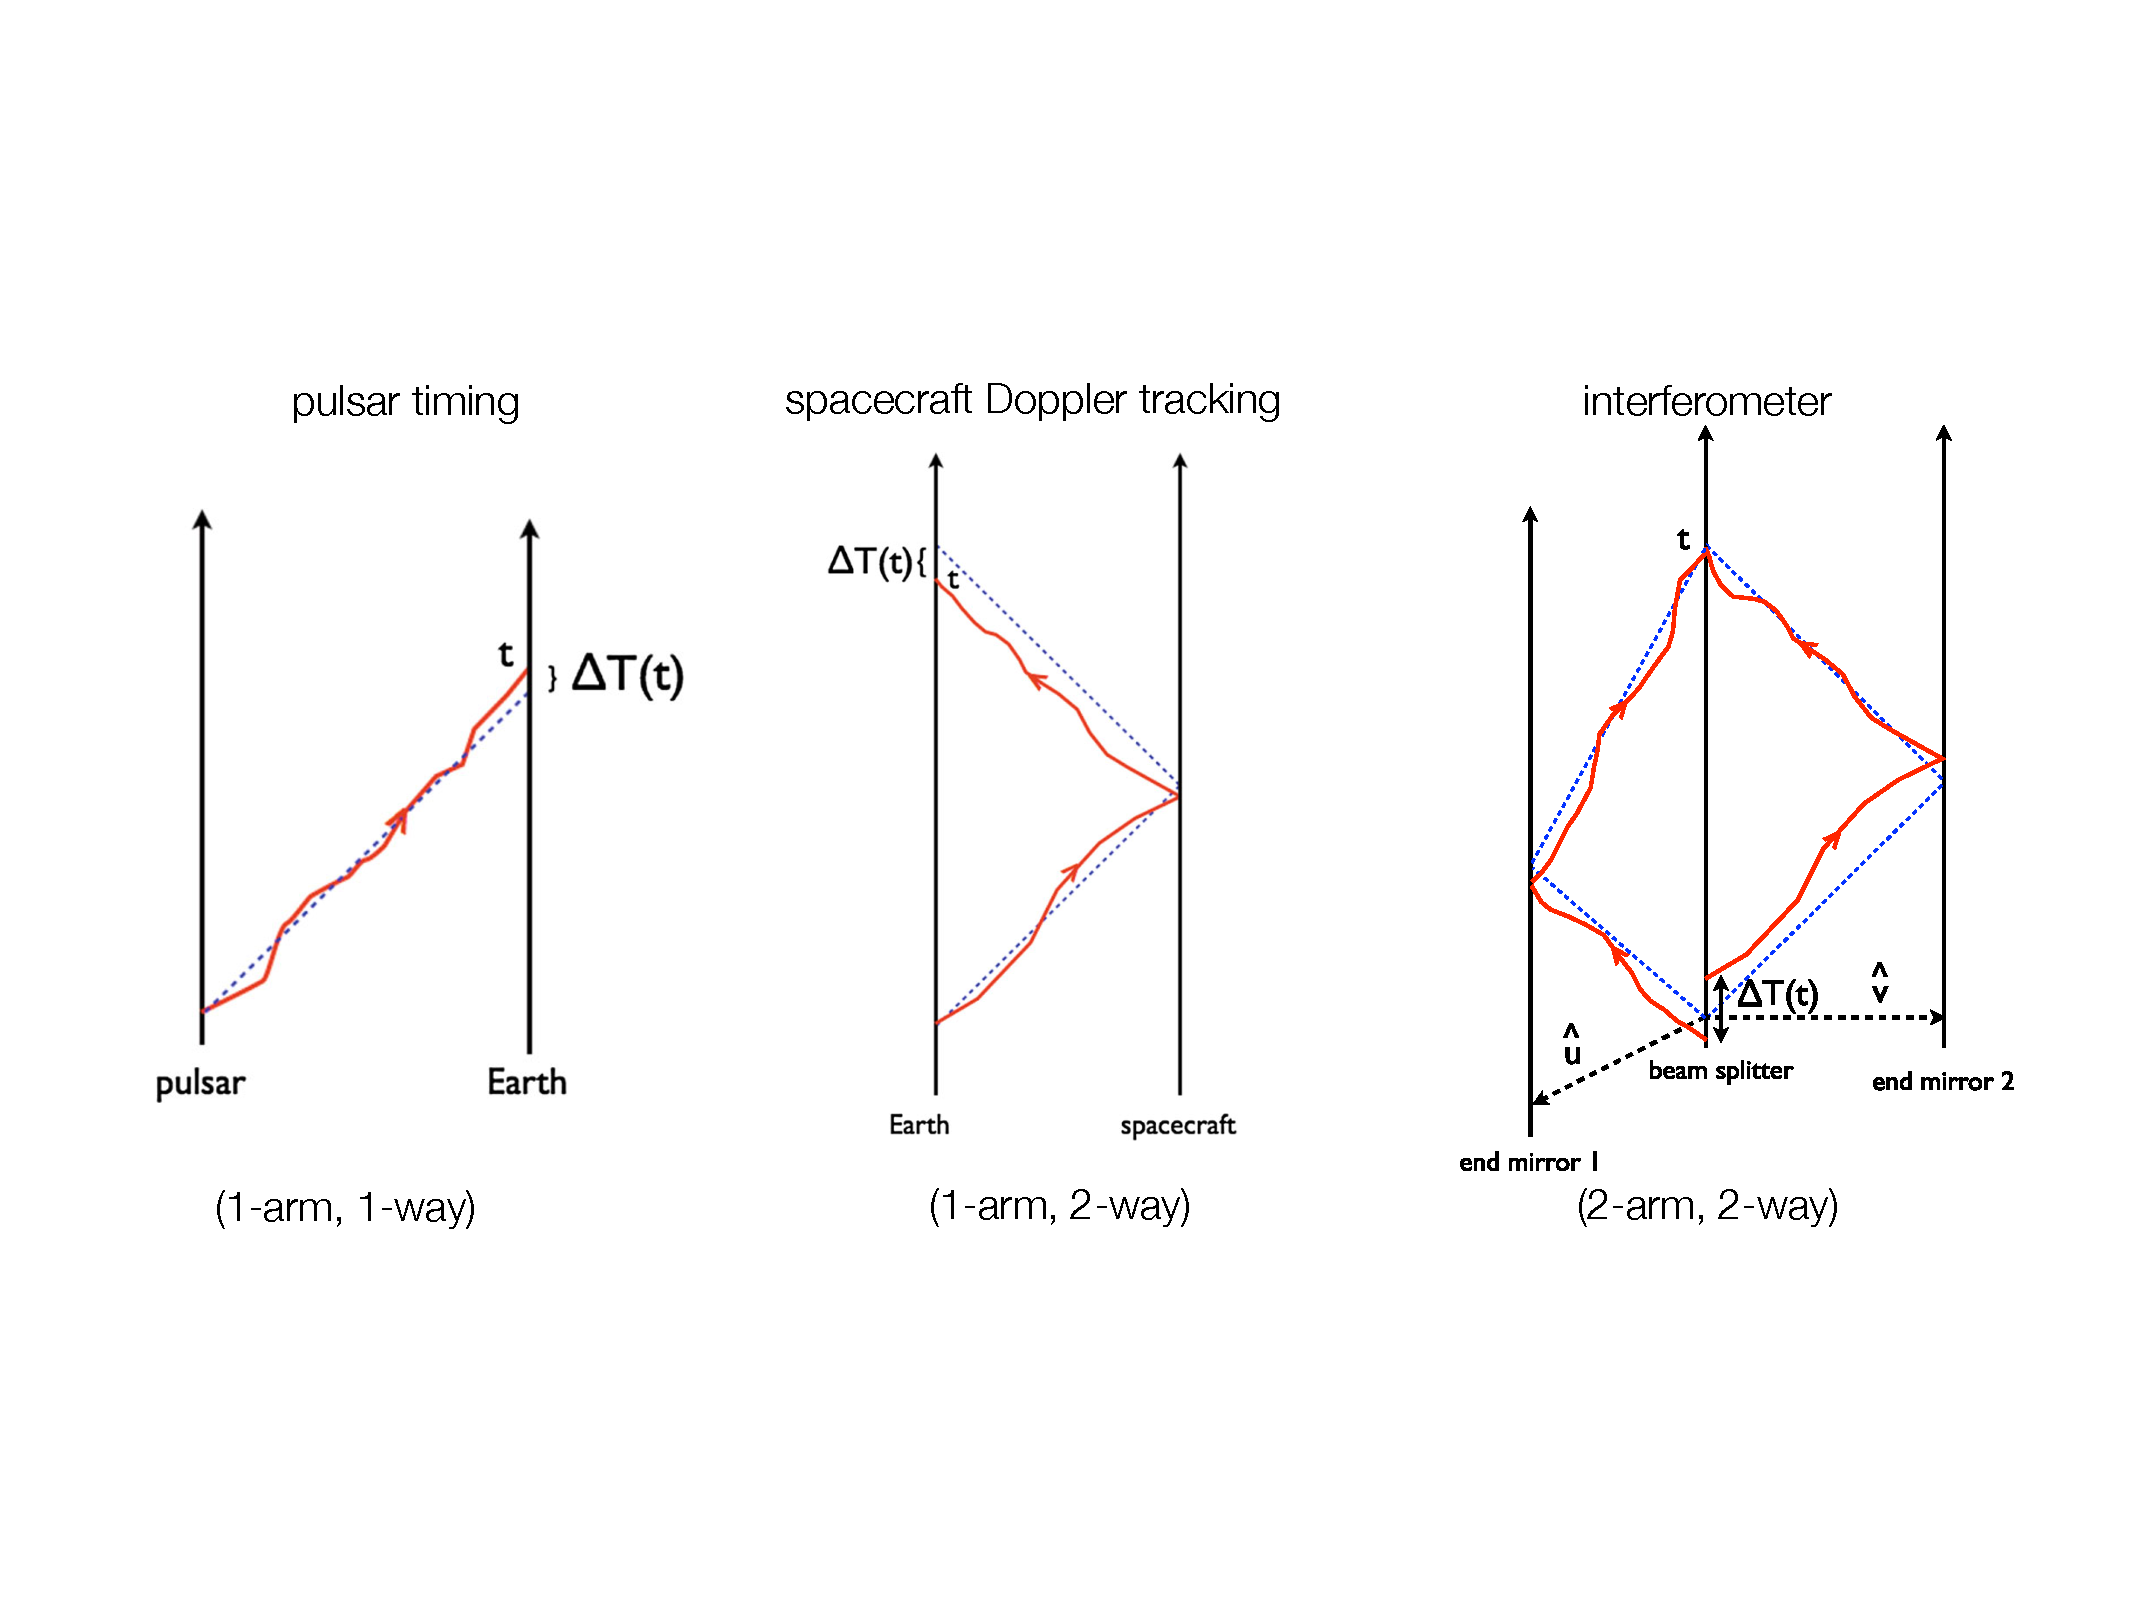
\includegraphics[width=\textwidth]{Figures/beam_detectors}
\caption{Spacetime diagram showing the response of beam
detectors to a passing GW.  
Left column: pulsar timing; middle column: spacecraft Doppler
tracking; right column: interferometer (ground or space-based).
A passing GW perturbs the path of the photon (red trajectory) 
relative to its nominal path in the absence of the wave 
(blue dotted line), leading to a 
difference in the expected arrival time of the photon.
(Figure adapted from \cite{Romano-Cornish:2017}.)}
\label{f:beam_detectors}
\end{center}
\end{figure}
%

In the literature, one might see the detector response
written in terms of strain $\Delta L(t)/L$, 
fractional Doppler frequency $\Delta v(t)/\nu_0$, or 
phase $\Delta\Phi(t)$, instead of the timing residual
$\Delta T(t)$.
Despite the apparent differences in the responses, 
they are all derivable from the change in light travel
time $\Delta T(t)$ via the relations:
%
\be
\begin{aligned}
&h(t)\equiv \Delta T(t)\quad &({\rm pulsar\ timing})\\
&h(t)\equiv \frac{\Delta L(t)}{L} = \frac{\Delta T(t)}{T}
\quad&({\rm LIGO,\ Virgo,\ }\cdots) \\
&h(t)\equiv \frac{\Delta\nu(t)}{\nu_0}=\frac{\D \Delta T(t)}{\D t}
\quad &({\rm spacecraft Doppler\ tracking})\\
&h(t)\equiv \Delta\Phi(t) = 2\pi \nu_0\,\Delta T(t)
\quad &({\rm LISA})\,.
\end{aligned}
\ee
%
Hence, once we know how to calculate the timing residual
response $\Delta T(t)$, we can easily calculate all the
other quantities listed above.

\subsection{Detector response functions}
\label{e:det_response}

Gravitational waves are weak.
As such, a GW detector act like a {\em linear} system,%
\footnote{It's a linear system 
since second-order and higher terms in the 
metric perturbations can be safely ignored.}
converting metric perturbations $h_{ab}(t,\vec x)$ 
to the detector output.
Mathematically, this is represented by the 
{\em convolution} of the metric perturbations with the 
{\em response function} of the detector:
%
\begin{equation}
h(t) = (\mb{R}*\mb{h})(t,\vec x)\equiv
\int_{-\infty}^\infty {\rm d}\tau
\int {\rm d}^3 y\>
R^{ab}(\tau,\vec y)h_{ab}(t-\tau, \vec x-\vec y)\,.
\end{equation}
%
Here $h(t)$ is the output of the detector at time $t$.
The vector $\vec x$ is the location of detector, and 
$R^{ab}(\tau,\vec y)$ is the {\em impulse repsonse}
of the detector.
Expanding $h_{ab}(t-\tau,\vec x-\vec y)$ as a sum of
plane waves \eqref{e:planewave}, and substituting 
this into the RHS of the above expression, we find that the 
Fourier transform $\tilde h(f)$ of $h(t)$ can be written as
%
\be
\tilde h(f)=\int {\rm d}^2\Omega_{\hat n}
\sum_{A=+,\times} R^A(f,\hat k)\,h_A(f,\hat k)\,,
\ee
%
where
%
\be
R^A(f,\hat k) \equiv R^{ab}(f,\hat k)e^A_{ab}(\hat k)
\ee
%
and
%
\be
R^{ab}(f,\hat k) \equiv e^{-i 2\pi f\hat k\cdot\vec x/c}\,
\int_{-\infty}^\infty {\rm d}\tau \int {\rm d}^3 y\>
R^{ab}(\tau,\vec y)\,e^{-i2\pi f(\tau-\hat k\cdot\vec y/c)}\,.
\ee
%
Note that $R^A(f,\hat k)$ is the 
detector response for a plane-wave
with frequency $f$, propagation direction $\hat k$, and polarization $A$.

\subsection{Examples}

We now calculate the detector response functions for a couple of
examples.

\subsubsection{Detector response for a one-arm, one-way detector}

For our first example, we will consider the timing response of a one-arm,
one-way beam detector, which is relevant for pulsar timing observations.
The geometry of the situation is shown in Figure~\ref{f:one_arm_one_way}.
%
\begin{figure}[htbp!]
\begin{center}
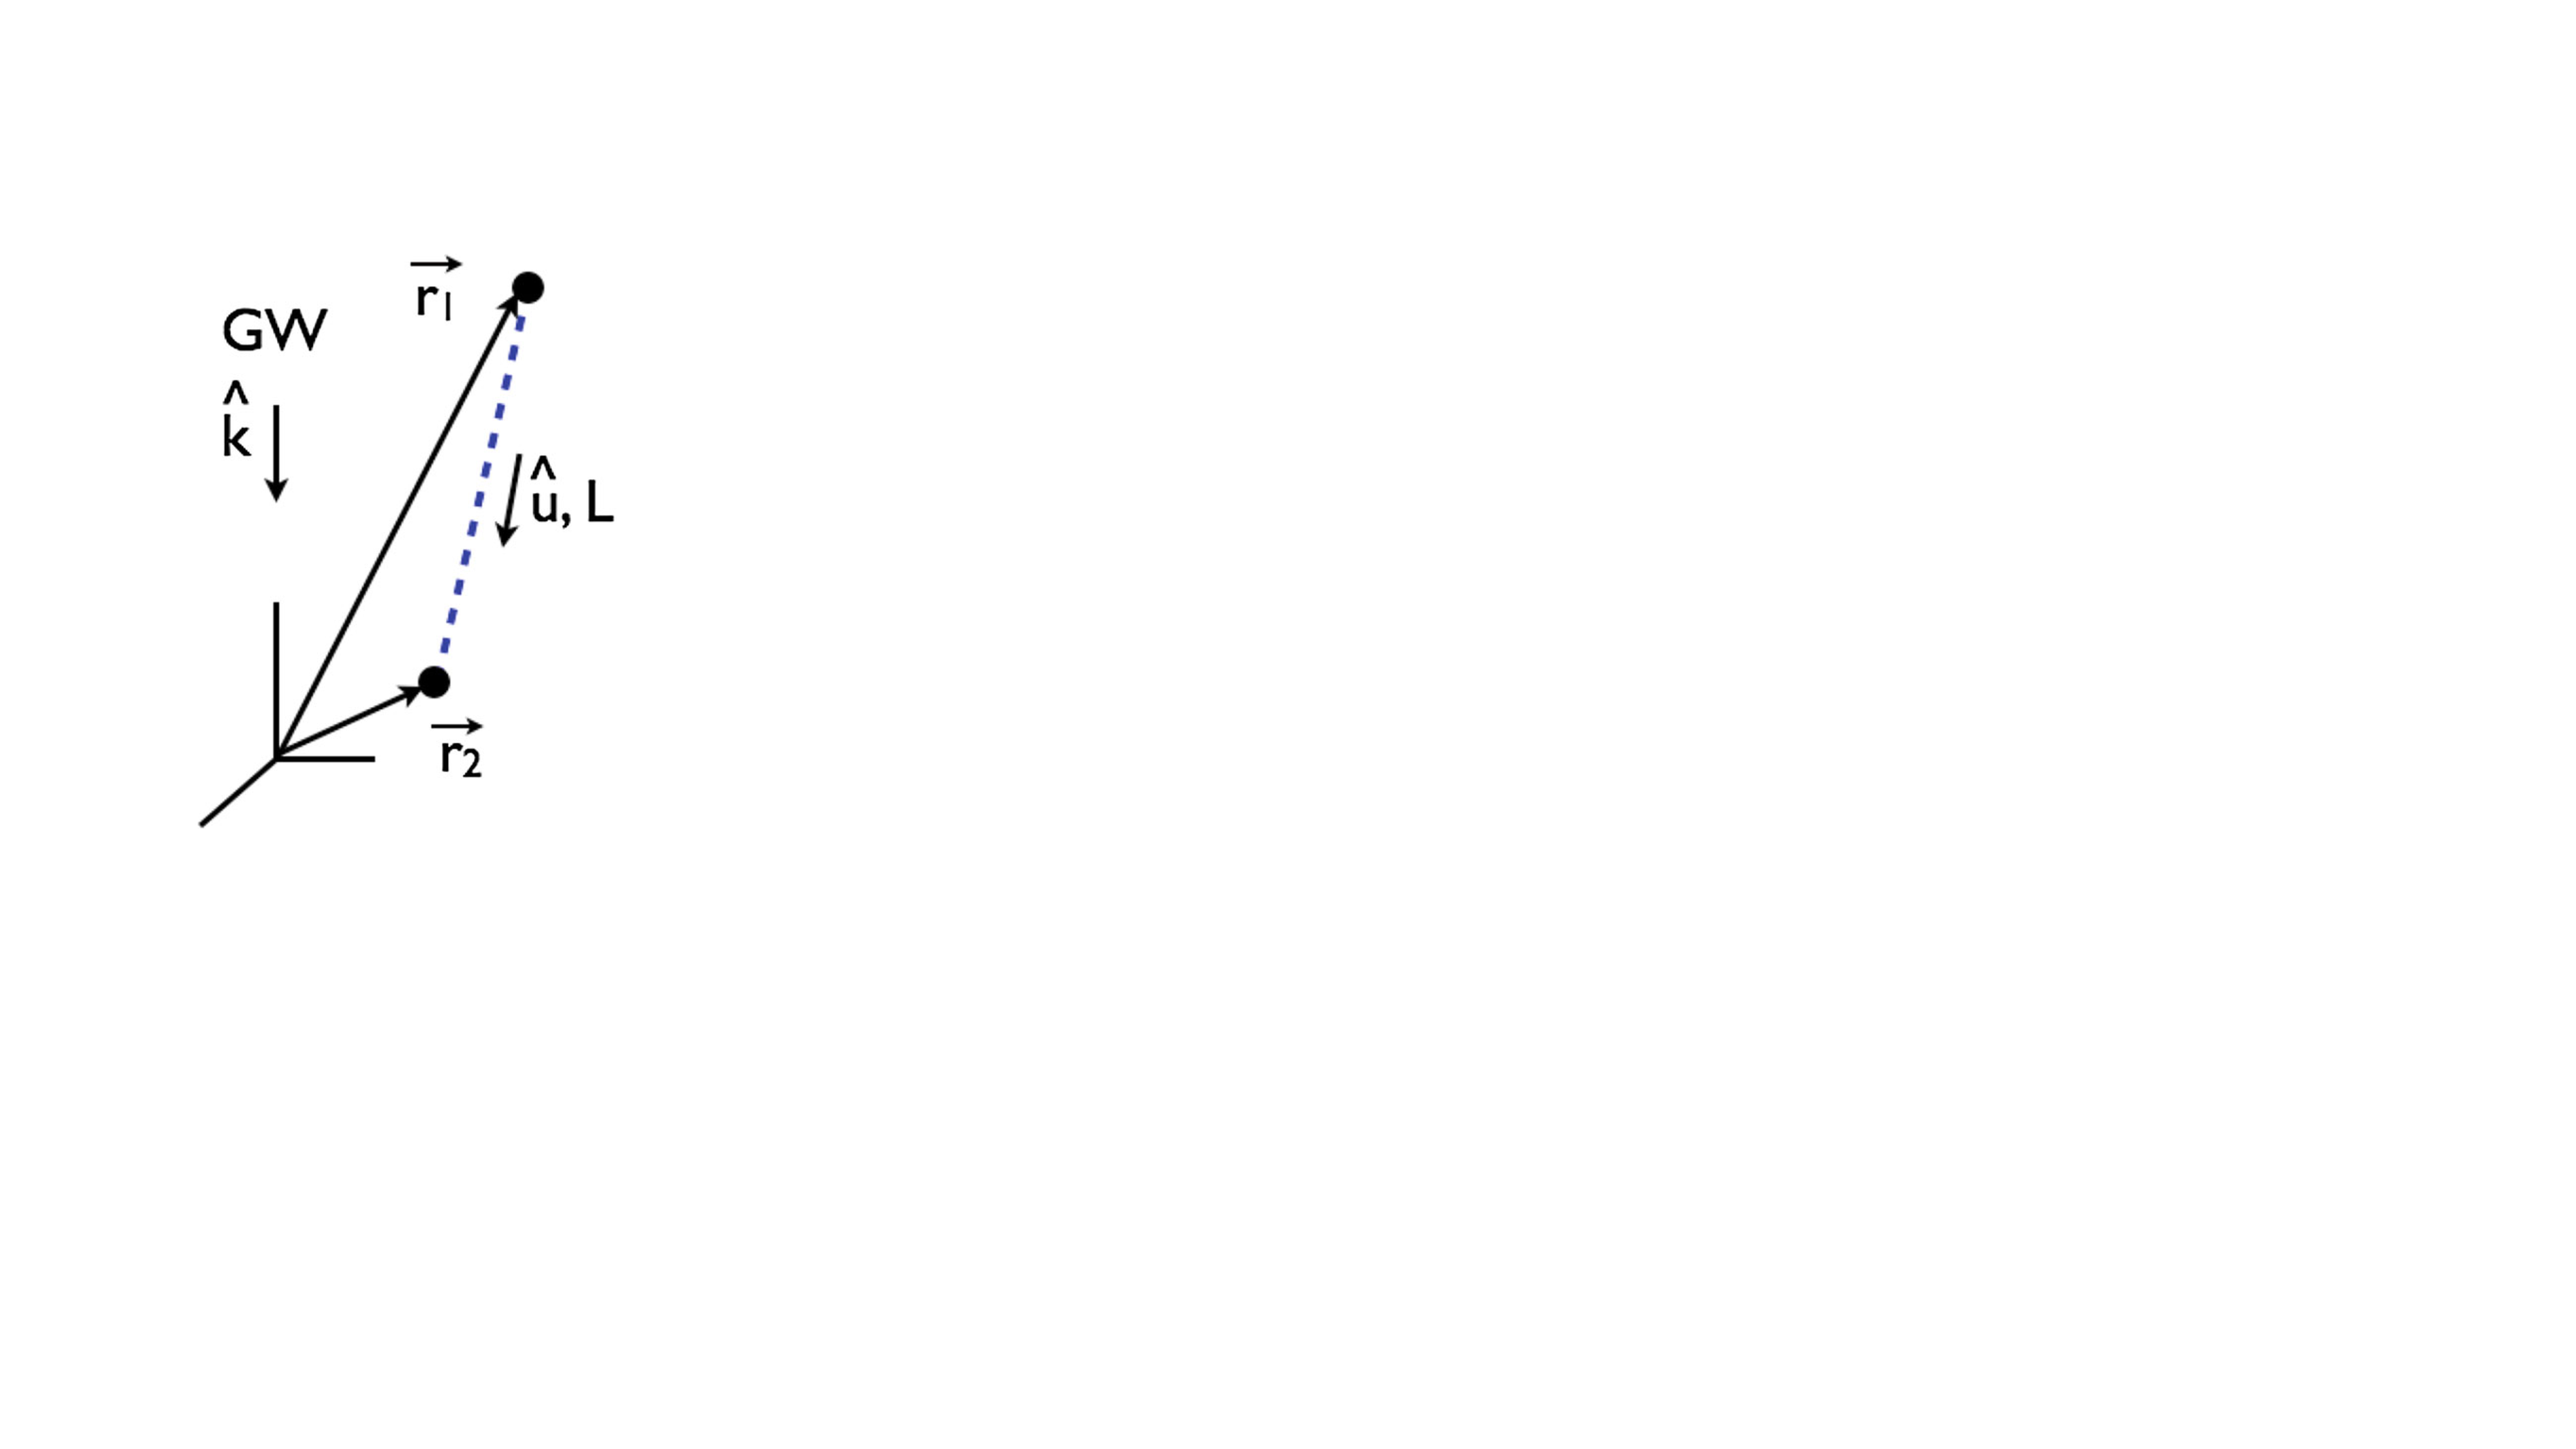
\includegraphics[width=0.2\textwidth]{Figures/one_arm_one_way}
\caption{Geometry for a one-arm, one-way beam detector, relevant for 
a pulsar timing residual measurement.
The GW propagates in the $\hat k$ direction; the electromagnetic wave
(e.g., a radio pulse from a pulsar) propagates in the $\hat u$ direction
(opposite of the direction to the pulsar, $\hat p=-\hat u$).} 
\label{f:one_arm_one_way}
\end{center}
\end{figure}
%
The timing residual response is then given by
\be
h(t)\equiv
\Delta T(t) = \frac{1}{2c} u^a u^b\int_0^L{\rm d}s\> h_{ab}(t(s),\vec x(s))\,,
\ee
%
where
%
\be
t(s) = (t-L/c) + s/c\,, \qquad
\vec x(s) = \vec r_1 + s\hat u
\ee
%
is a parametric representation of the photon path from the 
source ($s=0$) to the detector ($s=L$).
Note that we do not need to include any corrections to
the straight-line path for the photon given above, as the 
metric perturbations are already first-order and we 
can ignore all second-order terms in the calculation.

So to do the integral, we first substitute $t(s)$ and 
$\vec x(s)$ for $t$ and $\vec x$ in the plane-wave 
expansion for $h_{ab}(t,\vec x)$.
The $s$ dependence shows up only in the exponential:
%
\begin{equation}
\begin{aligned}
e^{i2\pi f(t(s)-\hat k\cdot\vec x(s)/c)}
&= e^{i2\pi f(t-L/c + s/c -\hat k\cdot(\vec r_1 + s\hat u)/c)}
\\
&= e^{i2\pi f(t-L/c -\hat k\cdot\vec r_1/c)}
e^{i2\pi f(1 -\hat k\cdot\hat u)s/c}\,,
\end{aligned}
\end{equation}
%
and the integral over $s$ is easy to do:
%
\be
\int_0^L {\rm d}s\>
e^{i2\pi f(1-\hat k\cdot\hat u)s/c}=
\frac{c}{i2\pi f}\frac{1}{1-\hat k\cdot\hat u}\left[e^{\frac{i2\pi f L}{c}
(1-\hat k\cdot\hat u)}-1\right]\,.
\ee
Then including all the other factors and rearranging terms, 
you should find (Exercise~\ref{exer:6}):
%
\be
R^A(f,\hat k) = \frac{1}{i2\pi f}\,
\frac{1}{2}u^a u^b e^A_{ab}(\hat k)\frac{1}{1-\hat k\cdot \hat u}\,
\left[ 1-e^{-\frac{i 2\pi fL}{c}(1-\hat k\cdot\hat u)}\right]
\,e^{-i2\pi f\hat k\cdot\vec r_2/c}\,.
\label{e:response_one_arm_one_way}
\ee
%
In the context of pulsar timing, the two terms in square brackets 
are called the {\em Earth term} and {\em pulsar term}, respectively.
The pulsar term encodes information about the phase of the GW at
the location of the pulsar.
It is usually ignored for stochastic background searches, as 
this term for different pulsars will not be correlated with one other
(since the spatial distance between two pulsars, of order kpc, 
is much greater than the wavelengths of the GWs that pulsar timing arrays are 
sensitive to, of order 10~light-years).

Both terms {\em are} important for LISA data analysis, however,
as the wavelengths of the GWs that LISA will be sensitive to
are of the same order of magnitude as the lengths of LISA's arms 
(i.e., the separation between the spacecraft).
For this case, one defines a {\em timing transfer function} for 
one-way photon propagation as
%
\be
\begin{aligned}
{\cal T}_{\vec u}(f,\hat k\cdot \hat u) 
&\equiv\frac{1}{i2\pi f}\frac{1}{1-\hat k\cdot\hat u}
\left[1-e^{-\frac{i2\pi f L}{c}(1-\hat k\cdot\hat u)}\right]
\\
&= \frac{L}{c}\,e^{-\frac{i\pi fL}{c}(1-\hat k\cdot\hat u)}
{\rm sinc}\left(\frac{\pi fL}{c}[1-\hat k\cdot\hat u]\right)\,,
\end{aligned}
\ee
%
where ${\rm sinc}\,x\equiv \sin x/x$.
Note that for normal incidence (i.e., $\hat k\cdot\hat u=0$), 
the timing transfer function has zeroes when $L$ is equal to 
an integer number of GW wavelengths $\lambda\equiv c/f$---i.e.,
when $fL/c$ equals an integer
(Figure~\ref{f:timing_transfer}).
%
\begin{figure}[htbp!]
\begin{center}
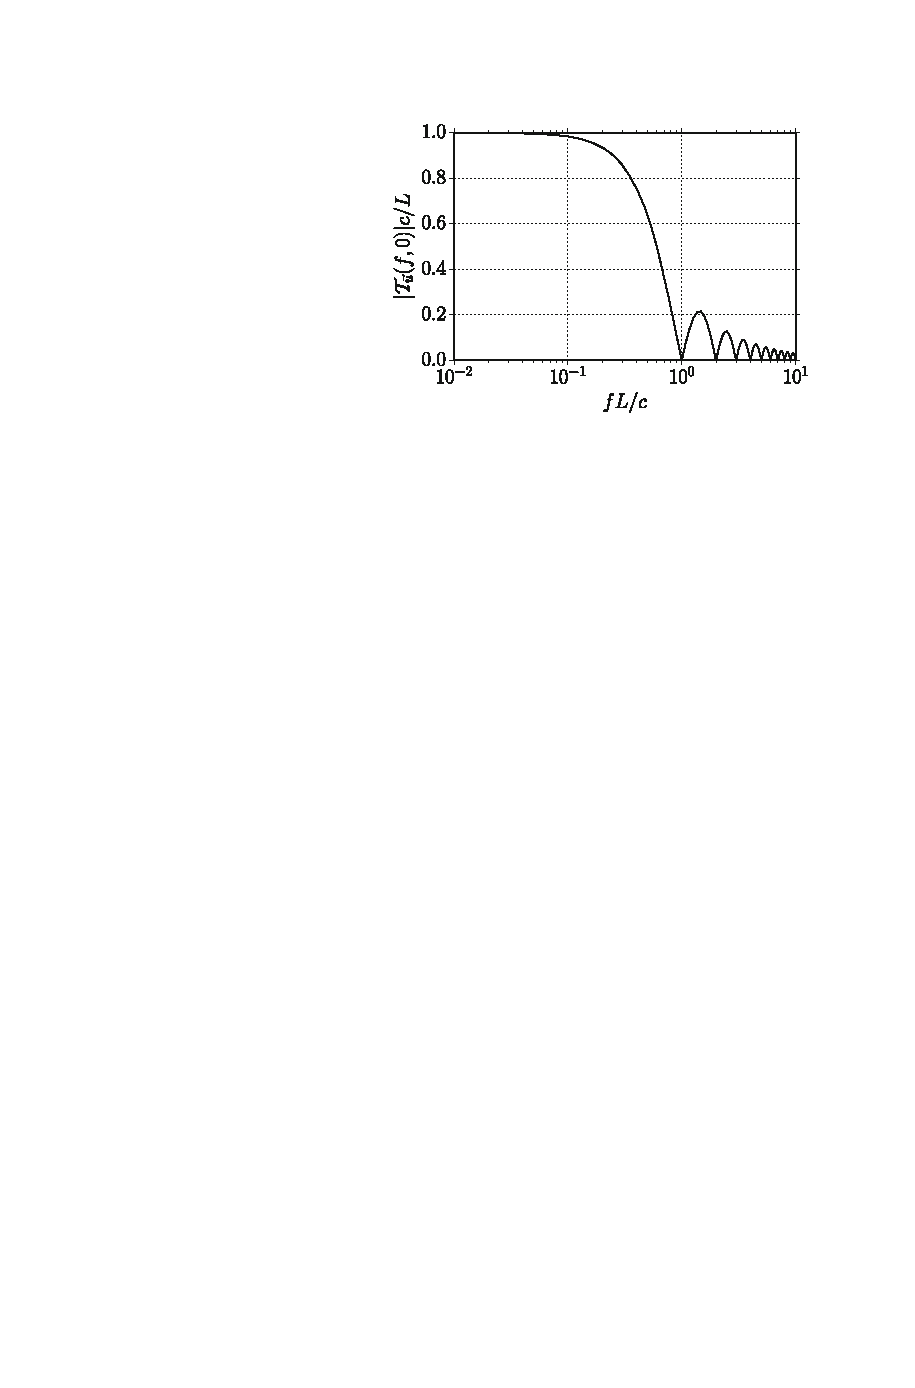
\includegraphics[width=0.5\textwidth]{Figures/timing_transfer}
\caption{Plot of the absolute value of the timing transfer 
function $|{\cal T}_{\vec u}(f,0)|$ for normal incidence.
Note the nulls in the response when $L$ equals an integer 
number of GW wavelengths $\lambda \equiv c/f$.}
\label{f:timing_transfer}
\end{center}
\end{figure}
%

Returning to \eqref{e:response_one_arm_one_way} and its 
application to pulsar timing analyses, 
note that the factor $1/(i2\pi f)$ goes away for the Doppler 
frequency response, $\Delta\nu(t)/\nu_0$, and that the
phase term $e^{-i2\pi f\hat k\cdot\vec r_2/c}$ equals one
if we take the $\vec r_2$ to be the origin of coordinates, e.g.,
at the solar system barycenter.
Thus, ignoring the pulsar term, the Doppler frequency 
response is given simply by
%
\be
F^A(\hat k) 
=\frac{1}{2}\frac{u^a u^b}{1-\hat k\cdot\hat u}\,e_{ab}^A(\hat k)\,.
\label{e:F^A(k)}
\ee
%
A plot of the root-summed-squared response (summed over the 
two polarizations)
is shown in Figure~\ref{f:one_arm_one_way_peanut} for the 
case $\hat u=-\hat z$ (or, equivalently, $\hat p=\hat z$ where 
$\hat p=-\hat u$ is the direction to the pulsar).
%
\begin{figure}[htbp!]
\begin{center}
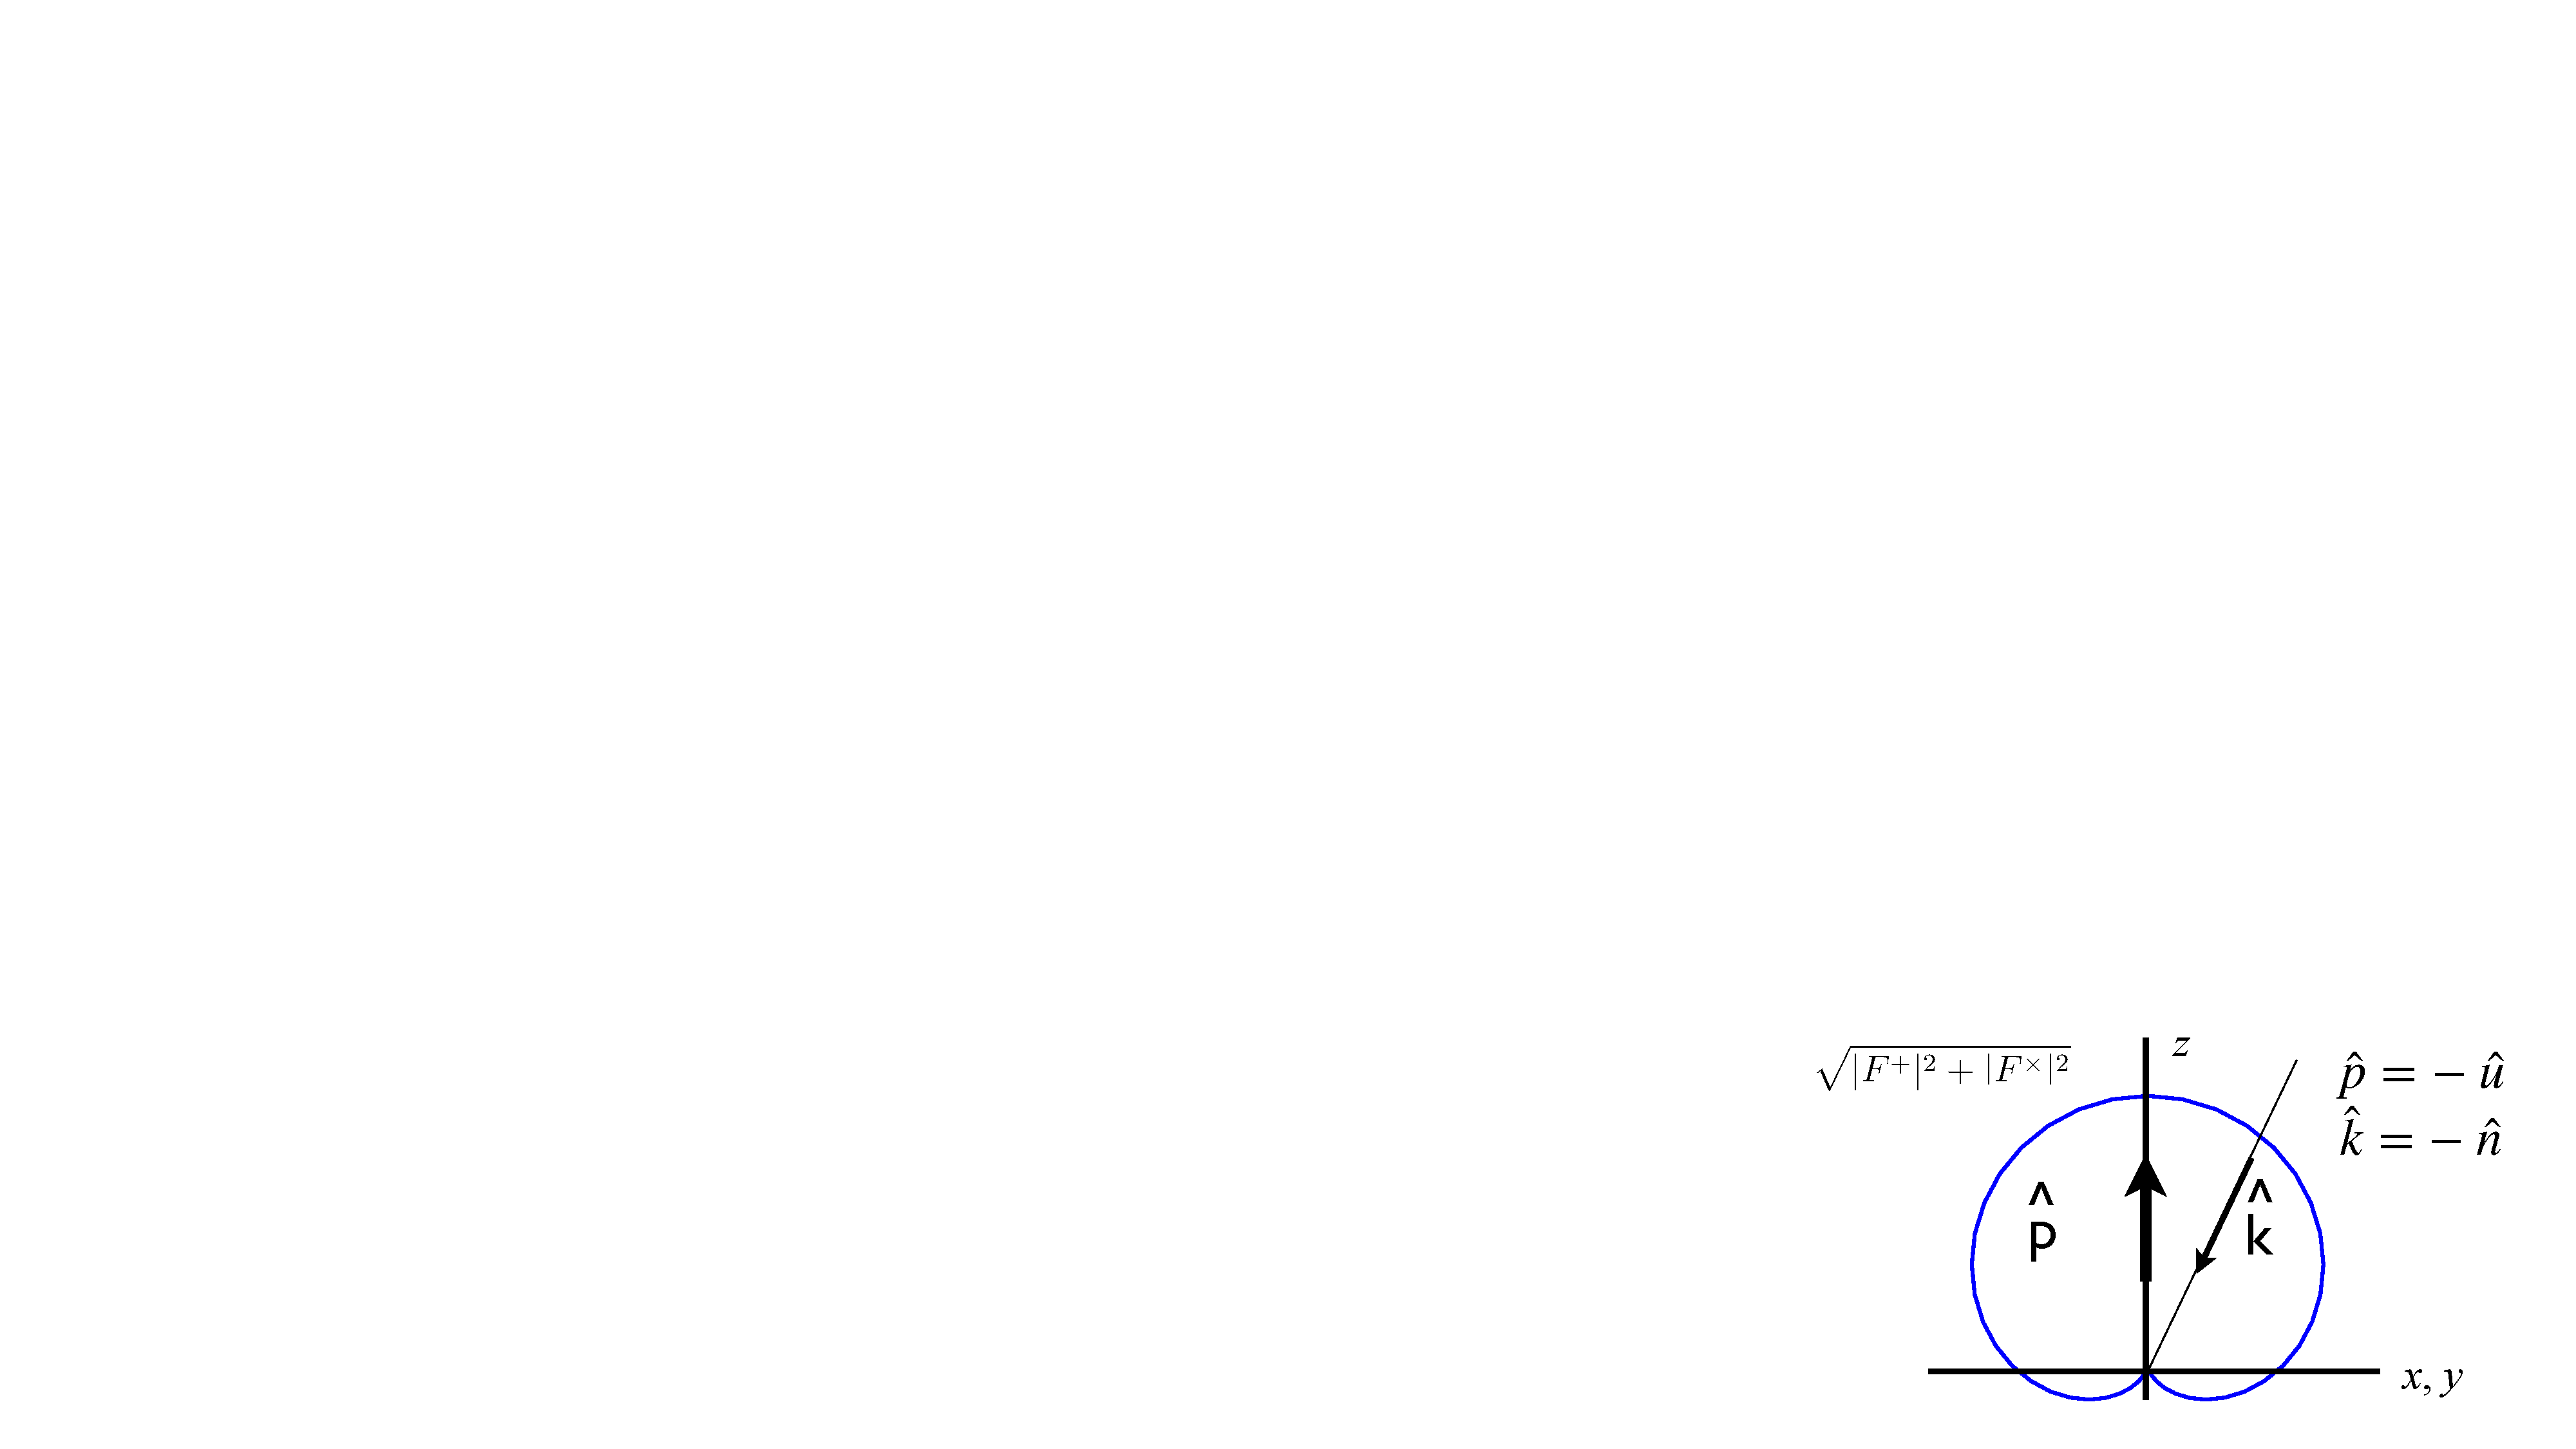
\includegraphics[width=0.4\textwidth]{Figures/one_arm_one_way_peanut}
\caption{Polarization-averaged Doppler frequency response
for pulsar timing, where we have ignored the pulsar term.
The response is axially symmetric around the $z$-axis, which
we've chosen to be the direction to the pulsar $\hat p=-\hat u$.}
\label{f:one_arm_one_way_peanut}
\end{center}
\end{figure}
%
The response is maximum when the GW and radio pulse propagate 
in the same direction---i.e., when $\hat k=\hat u$.
It is zero when they propagate in opposite directions.
These results follow from 
%
\be
\begin{aligned}
&u^a u^b e^+_{ab}(\hat k) 
= \sin^2\theta = (1-\cos\theta)(1+\cos\theta)\,,
\\
&u^a u^b e^\times_{ab}(\hat k)=0\,,
\\
& 1-\hat k\cdot\hat u = 1-\cos\theta\,,
\end{aligned}
\ee
%
for which
%
\be
F^+(\hat k) = \frac{1}{2}(1+\cos\theta)\,,
\qquad
F^\times(\hat k) = 0\,.
\label{e:FA_Earth_z}
\ee
%
Here $\theta$ is the angle between $\hat k$ and $\hat u$
(which is the usual polar angle measured from the $z$-axis).

Note that if we include the pulsar term in the response,
then $F^A(\hat k)$ in \eqref{e:FA_Earth_z} 
should be multiplied 
by a term proportional to $\sin(\pi f L[1-\cos\theta]/c)$.
This introduces a null at $\theta=0$ and at other values 
of $\theta$ satisfying
%
\be
\cos\theta = 1-\frac{nc}{fL}\,,
\qquad n=0,1,\cdots\,,{\rm int}[2fL/c]\,.
\ee
%
In Figure \ref{f:one_arm_one_way_peanut_full} we show
the full root-summed-squared response 
including the pulsar term,
taking $fL/c=20$ for illustration purposes.
(For most pulsars, $fL/c$ will be of order 100 
or more, as the distance to typical pulsars is 
of order a kpc or more.)
The response without the pulsar term 
(Figure~\ref{f:one_arm_one_way_peanut}) is also
shown for comparison.
%
\begin{figure}[htbp!]
\begin{center}
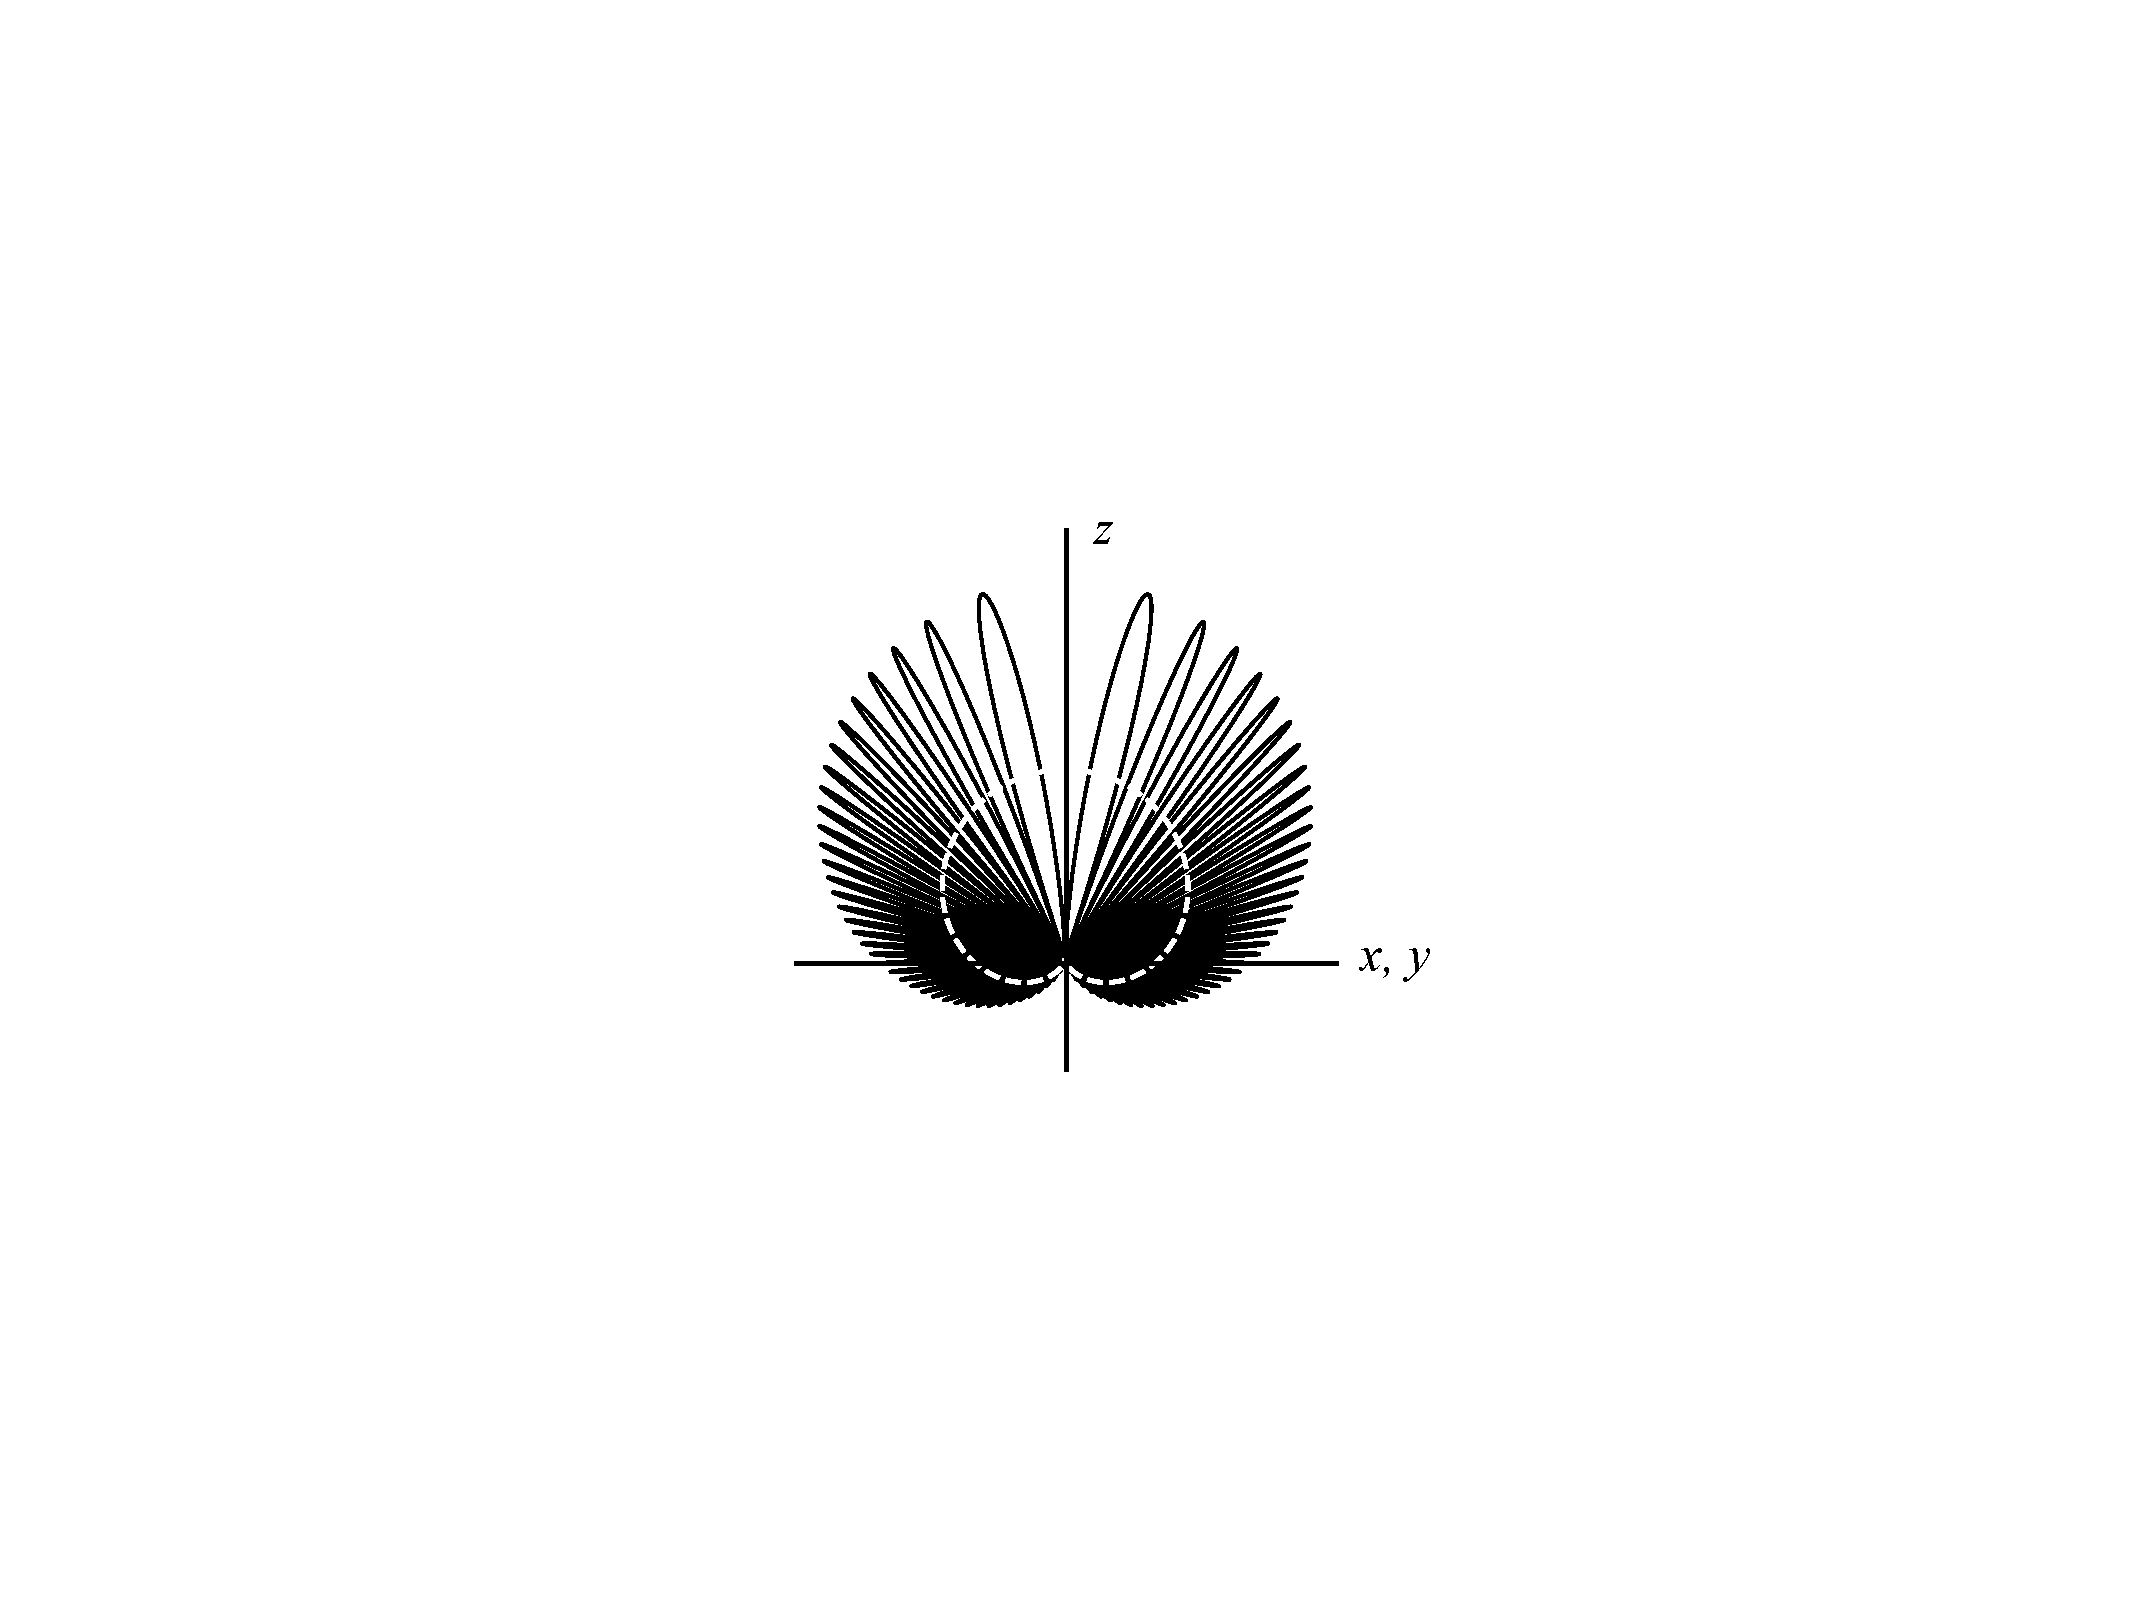
\includegraphics[width=0.4\textwidth]{Figures/pulsarPeanutComparison}
\caption{Same as Figure~\ref{f:one_arm_one_way_peanut} but 
including the pulsar term and taking $fL/c=20$.
The response without the pulsar term is shown as a 
dashed-white curved for comparison.}
\label{f:one_arm_one_way_peanut_full}
\end{center}
\end{figure}
%

%%%%%%%%%%%%%%%%%%%%%%%%%%%%%%
\subsubsection{Detector response for a laser interferometer 
in the short-antenna limit}

Another simple example of a detector response function is
for a equal-arm laser interferometer, like LIGO, in the 
{\em short-antenna} (or long-wavelength) 
approximation (Figure~\ref{f:LHO_geometry}).
%
\begin{figure}[htbp!]
\begin{center}
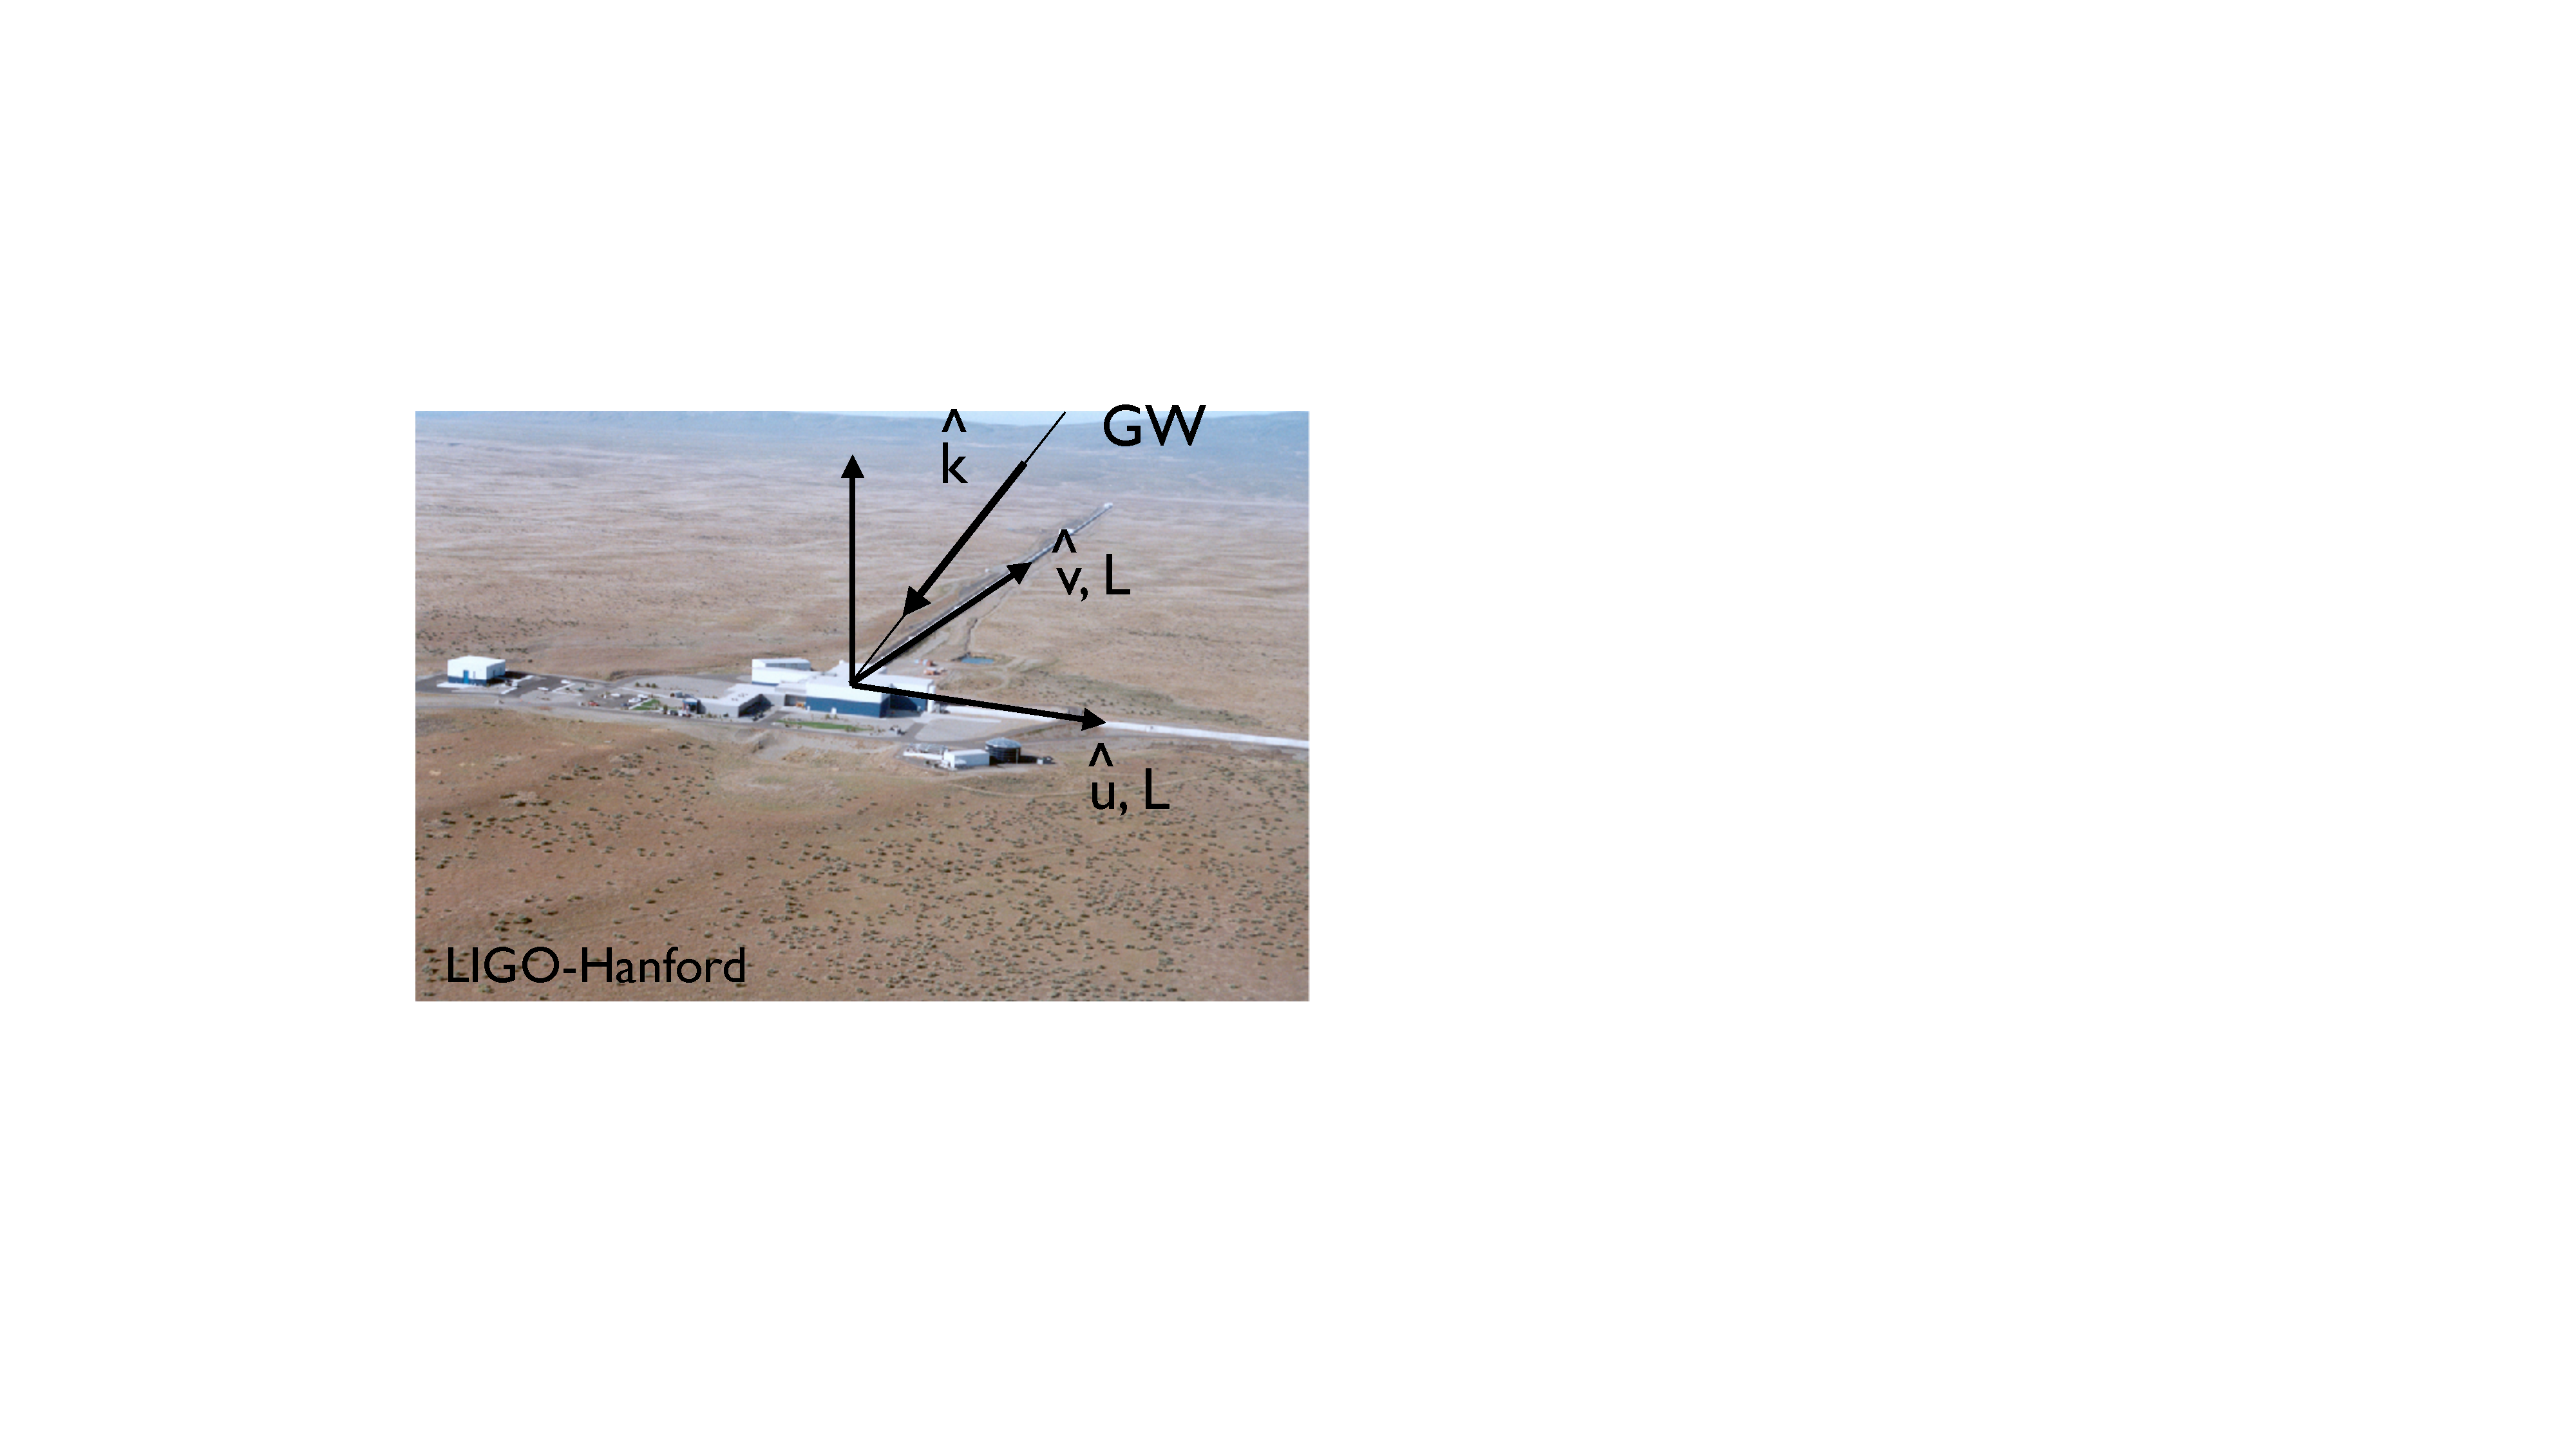
\includegraphics[width=0.6\textwidth]{Figures/LHO_geometry}
\caption{Geometry for a ground-based interferometer GW response
calculation.
(Shown here is the LIGO Hanford Observatory (LHO), 
in Hanford, WA.)
The GW propagates in the $\hat k$ direction;
$\hat u$, $\hat v$ are unit vectors that point along the 
two arms of the interferometer.
In the short-antenna approximation, the length $L$ of the 
arms does not enter the expression for the strain response.}
\label{f:LHO_geometry}
\end{center}
\end{figure}
%
This approximation is valid when the wavelength of the GW is 
much larger than the dimensions of the detector.  
Then, the GW phase is effectively constant as a photon
travels down an back an interferometer arm.
The integral over the photon path is simply proportional
to the nominal round-trip propagation time $2L/c$.
Defining the strain response of the interferometer as
%
\be
h(t) = \frac{1}{2}\left(
\frac{\Delta T_{\vec u,\, {\rm roundtrip}}(t)}{T}
-
\frac{\Delta T_{\vec v,\, {\rm roundtrip}}(t)}{T}
\right)
\ee
%
one can show that
%
\be
R^A(f,\hat k)\simeq\frac{1}{2}\left(u^au^b-v^av^b\right)\,e^A_{ab}(\hat k).
\ee
%
The quantity multiplying $e^A_{ab}(\hat k)$ in the 
expression for the reponse function above is called the 
{\em detector tensor}
%
\be
D^{ab}\equiv\frac{1}{2}\left(u^a u^b - v^a v^b\right)\,.
\ee
%
Plots of the {\em beam pattern functions}
$|R^+(f,\hat k)|$, $|R^\times(f,\hat k)|$ for the 
two polarizations individually, and the 
root-summed-squared response (summed over both polarization)
%$\sqrt{|R^+(f,\hat k)|^2 + |R^\times(f,\hat k)|^2}$
are shown in Figure~\ref{f:LIGO_beam_patterns}.
The last plot showing the root-summed-squared response 
is sometimes called the LIGO ``peanut".
It illustrates that a laser-interferometer in the 
short-antenna approximation is a very blunt instrument,
being senstive to a very large portion of the sky. 
The only nulls are in the plane spanned by the arms, 
in the directions of the perpendicular bisectors of 
the arms.
%
\begin{figure}[htbp!]
\begin{center}
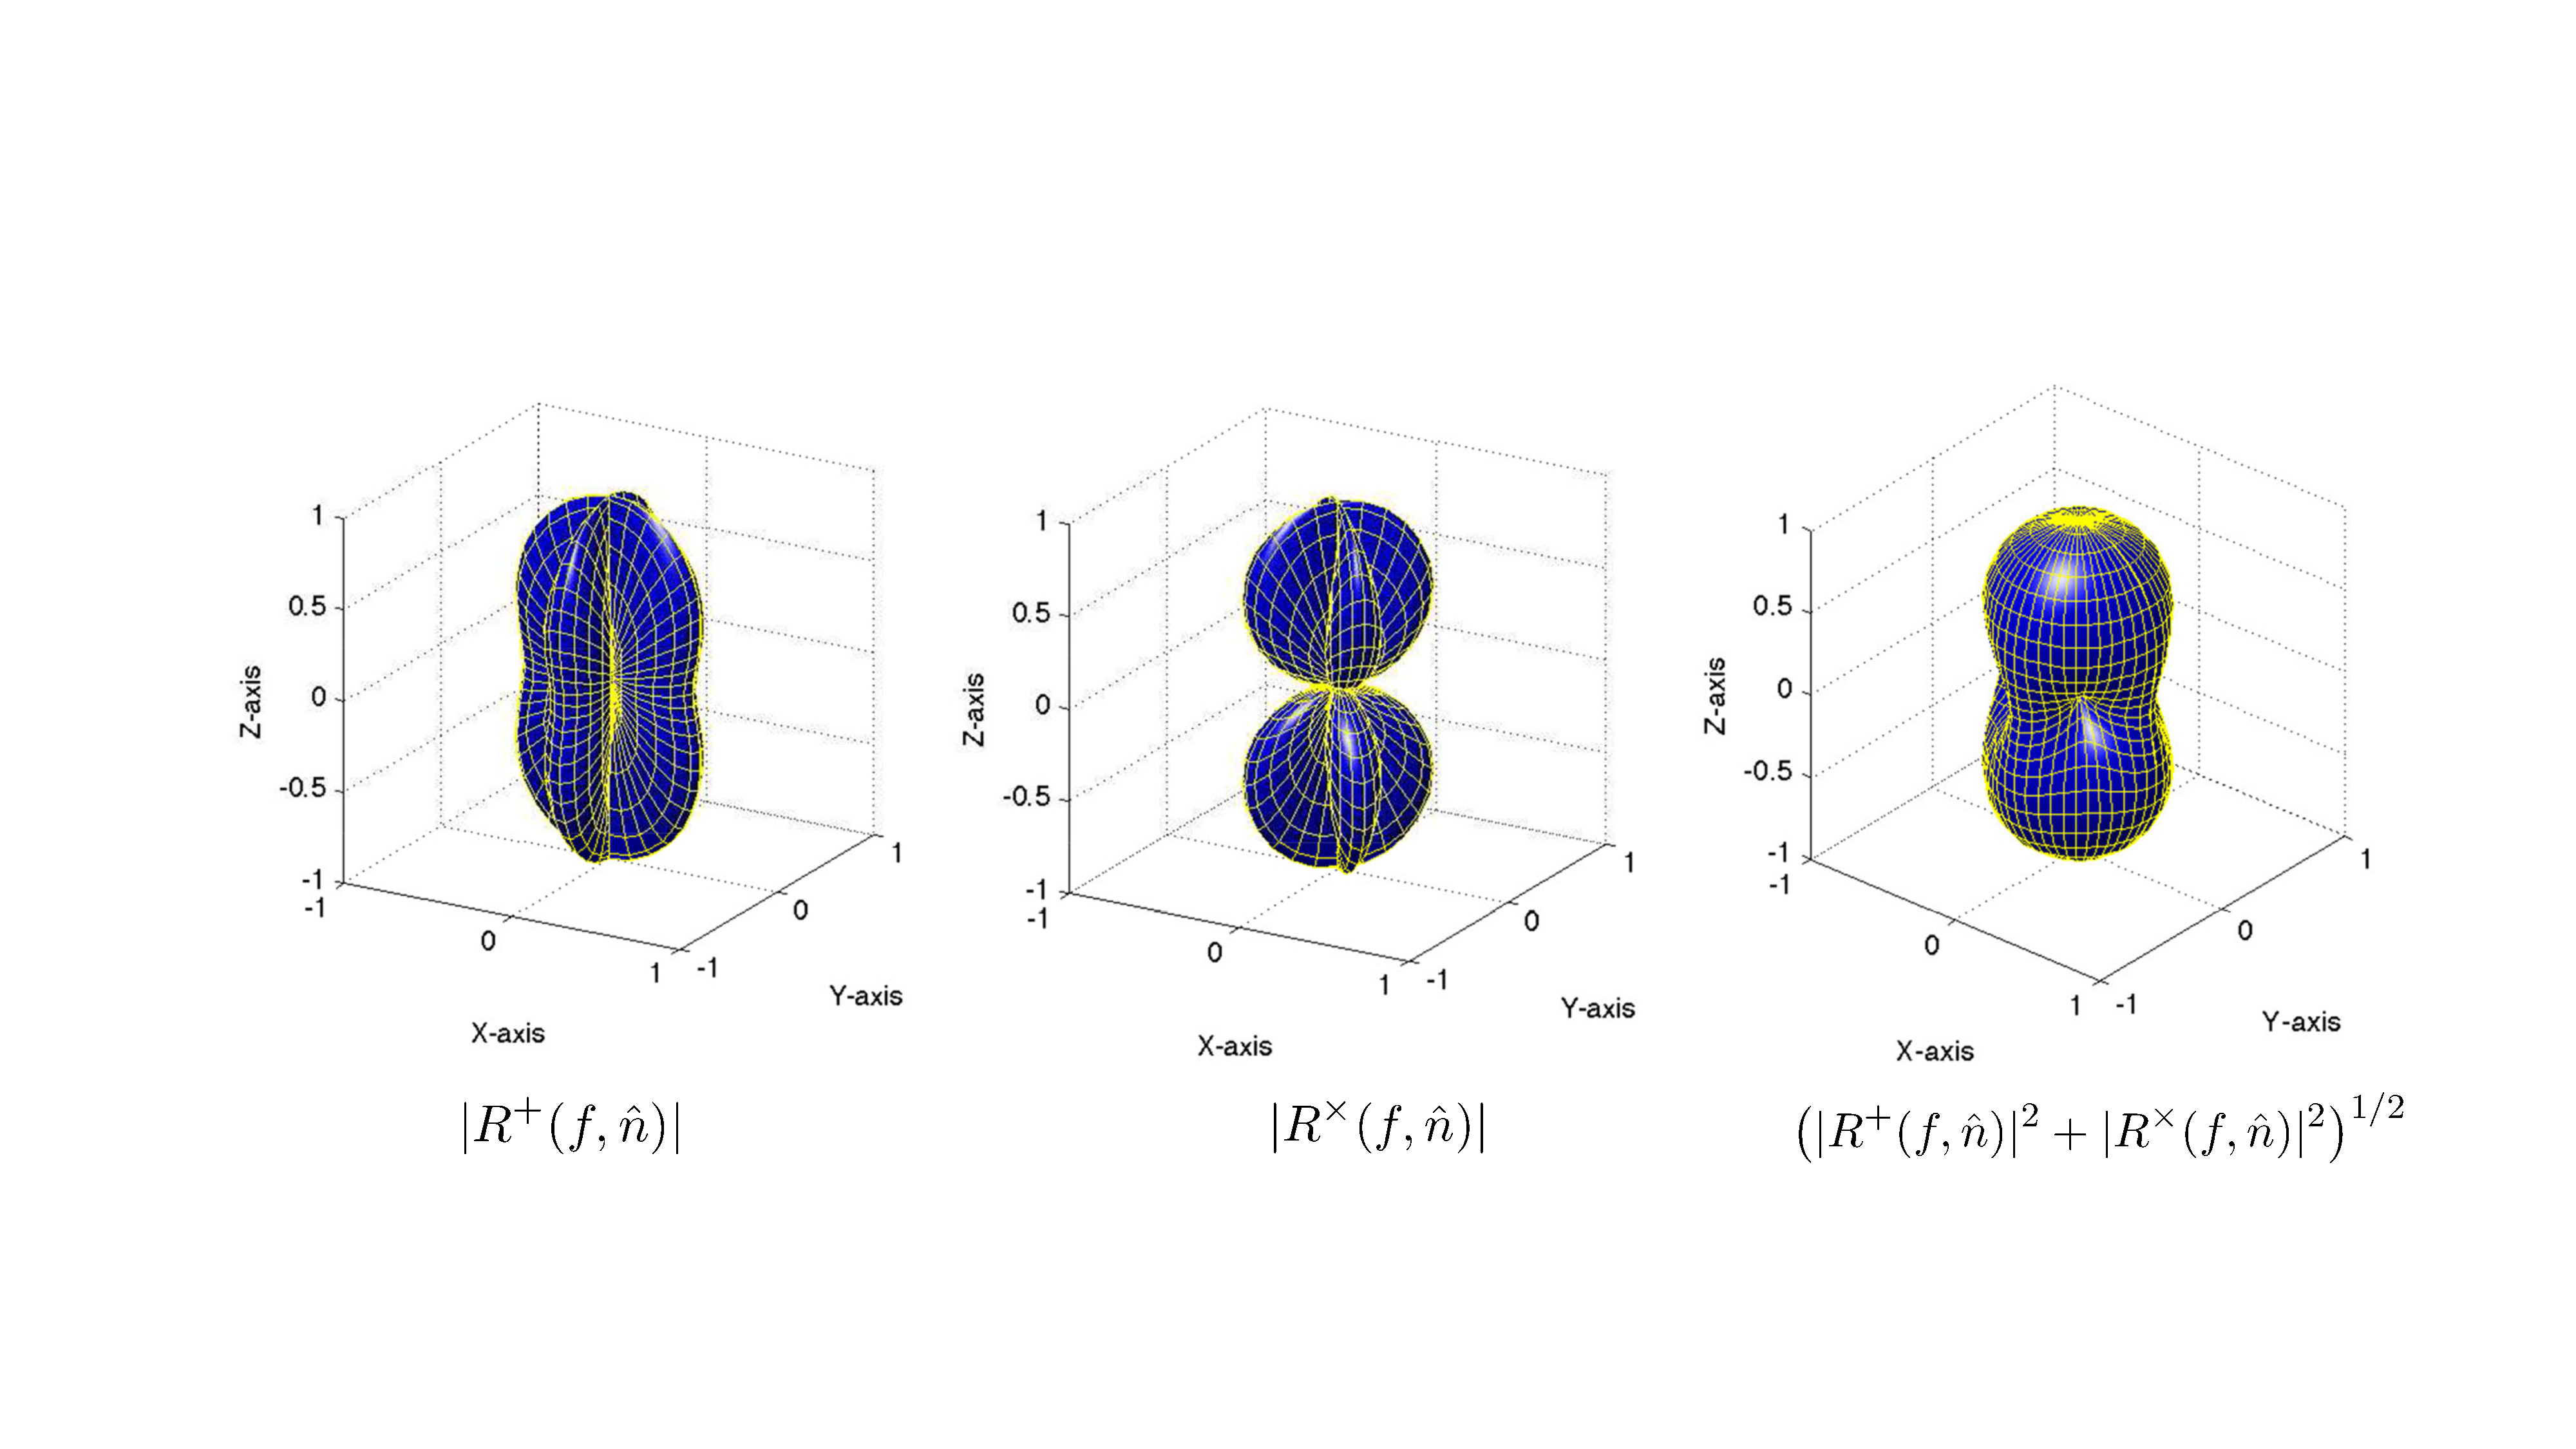
\includegraphics[width=\textwidth]{Figures/LIGO_beam_patterns}
\caption{Beam pattern functions for a ground-based interferometer
like LIGO in the short-antenna approximation---i.e., $f\lesssim {\rm few\ kHz}$.
The vertex of the interferometer is at the origin of coordinates,
and interferometer arms are assumed to be orthogonal pointing along
the $x$ and $y$ directions.}
\label{f:LIGO_beam_patterns}
\end{center}
\end{figure}
%

%%%%%%%%%%%%%%%%%%%%%%%%%%%%%%%%%%%%%%%%%%%%%%%%%%%%%%
\section{Non-trivial correlations}
\label{s:nontrivial_correlations}

In this section, we describe how to correlate the outputs
of two detectors, taking into account their non-trivial
response to GWs.

\subsection{Overlap function}

Detectors in different locations and with different 
orientations respond differently to a passing GW.
The {\em overlap function} encodes the reduction in 
sensitivity of a cross-correlation analysis due to 
the separation and misalignment of the detectors.

Let $I$ and $J$ label two detectors, and let 
$h_I(t)$ and $h_J(t)$ denote the corresponding response
of these detectors to an unpolarized and isotropic
GW background.
The expected correlation of the two detector outputs
can then be written as
%
\be
\langle h_I(t)h_J(t')\rangle 
= \frac{1}{2}\int_{-\infty}^\infty{\rm d}f\>
e^{i2\pi f(t-t')}\Gamma_{IJ}(f)S_h(f)\,,
\label{e:Gamma-time}
\ee
%
where $S_h(f)$ is the (1-sided) strain power spectral density
of the GWB, cf.~\eqref{e:quad_iso} and \eqref{e:S_h_and_Omega_gw}, 
and $\Gamma_{IJ}(f)$ is the overlap function: 
%
\be
\Gamma_{IJ}(f) 
= \frac{1}{8\pi}\int {\rm d}^2\Omega_{\hat k}\> 
\sum_A R_I^A(f,\hat k) R_J^{A}{}^{*}(f,\hat k)\,.
\label{e:Gamma}
\ee
%
The interpretation of $\Gamma_{IJ}(f)$ as encoding 
the reduction in sensitivity of a cross-correlation
analysis due to physical separation and relative
orientation of the detectors
is most easily seen in the frequency domain, where
%
\be
\langle \tilde h_I(f)\tilde h_J^*(f')\rangle 
= \frac{1}{2}\delta(f-f')\Gamma_{IJ}(f)S_h(f)\,.
\label{e:Gamma-freq}
\ee
%
From this expression, we see that $\Gamma_{IJ}(f)$ 
is a transfer function between the strain power 
$S_h(f)$ in the GWB and the detector cross-power.
(The factor of $1/2$ arises since $S_h(f)$ is a 
1-sided power spectral density; the Dirac delta
function $\delta(f-f)$ is a consequence of 
stationarity.)

For statistically anisotropic backgrounds, it 
turns out that the integrand of 
$\Gamma_{IJ}(f)$ is the most important quantity for
describing the cross-correlation.
This is because for this case
%
\be
\langle \tilde h_I(f)\tilde h_J^*(f')\rangle 
= \frac{1}{4}\delta(f-f')\int {\rm d}^2\Omega_{\hat k}\> 
\sum_A R_I^A(f,\hat k) R_J^{A}{}^{*}(f,\hat k) {\cal P}(f,\hat k)\,,
\label{e:aniso-corr}
\ee
%
where ${\cal P}(f,\hat k)$ is the GW power on the 
sky, coming from direction $\hat n=-\hat k$; see \eqref{e:quad_aniso}
and \eqref{e:Sh_aniso}.
One typically expands 
${\cal P}(f,\hat k)$ in terms of spherical harmonics 
%
\be
{\cal P}(f,\hat k) = \sum_{l=0}^\infty\sum_{m=-l}^l
{\cal P}_{lm}(f)Y_{lm}(\hat k)\,,
\ee
%
for which \eqref{e:aniso-corr} becomes
%
\be
\langle \tilde h_I(f)\tilde h_J^*(f')\rangle 
= \frac{1}{2}\delta(f-f')\sum_{l=0}^\infty\sum_{m=-l}^l
\Gamma_{IJ,lm}(f){\cal P}_{lm}(f)\,.
\label{e:Gamma-freq-aniso}
\ee
%
with
%
\be
\Gamma_{IJ,lm}(f) \equiv 
\frac{1}{2}
\int{\rm d}^2\Omega_{\hat k}\>
\sum_A R_I^A(f,\hat k) R_J^{A}{}^{*}(f,\hat k) 
Y_{lm}(\hat k)\,.
\ee
%
So up to a factor of $1/4\pi$, the spherical harmonic 
components of the integrand of the overlap function
\eqref{e:Gamma} encode the reduction in sensitivity
when doing a cross-correlation for anisotropic backgrounds.
Interested readers can find much more discussion
about anisotropic background in Section~7 of
\cite{Romano-Cornish:2017}, and references to the
original work cited therein.

%%%%%%%%%%%%%%%%%%%%%%%%%%%%%%%
\subsection{Examples}

Given \eqref{e:Gamma} for $\Gamma_{IJ}(f)$ and 
explicit expressions for the response functions 
$R^A_I(f,\hat k)$ for different detectors, we can 
now calculate the overlap function for different 
detector pairs.

\subsubsection{Overlap function for a pair of laser
interferometers in the short-antenna limit}

Our first example will be the overlap function 
for pairs of laser interferometers in the short-antenna
approximation.
For concreteness, we will consider the 
LIGO Hanford-LIGO Livingston detector pair (which we will
denote LHO-LLO)
and the LIGO Hanford-Virgo (LHO-Virgo) detector pair.
Plots of these overlap functions, normalized to unity
for coincident and coaligned detectors 
(denoted $\gamma(f)$) are shown in Figure~\ref{f:orfs}.
%
\begin{figure}[htbp!]
\begin{center}
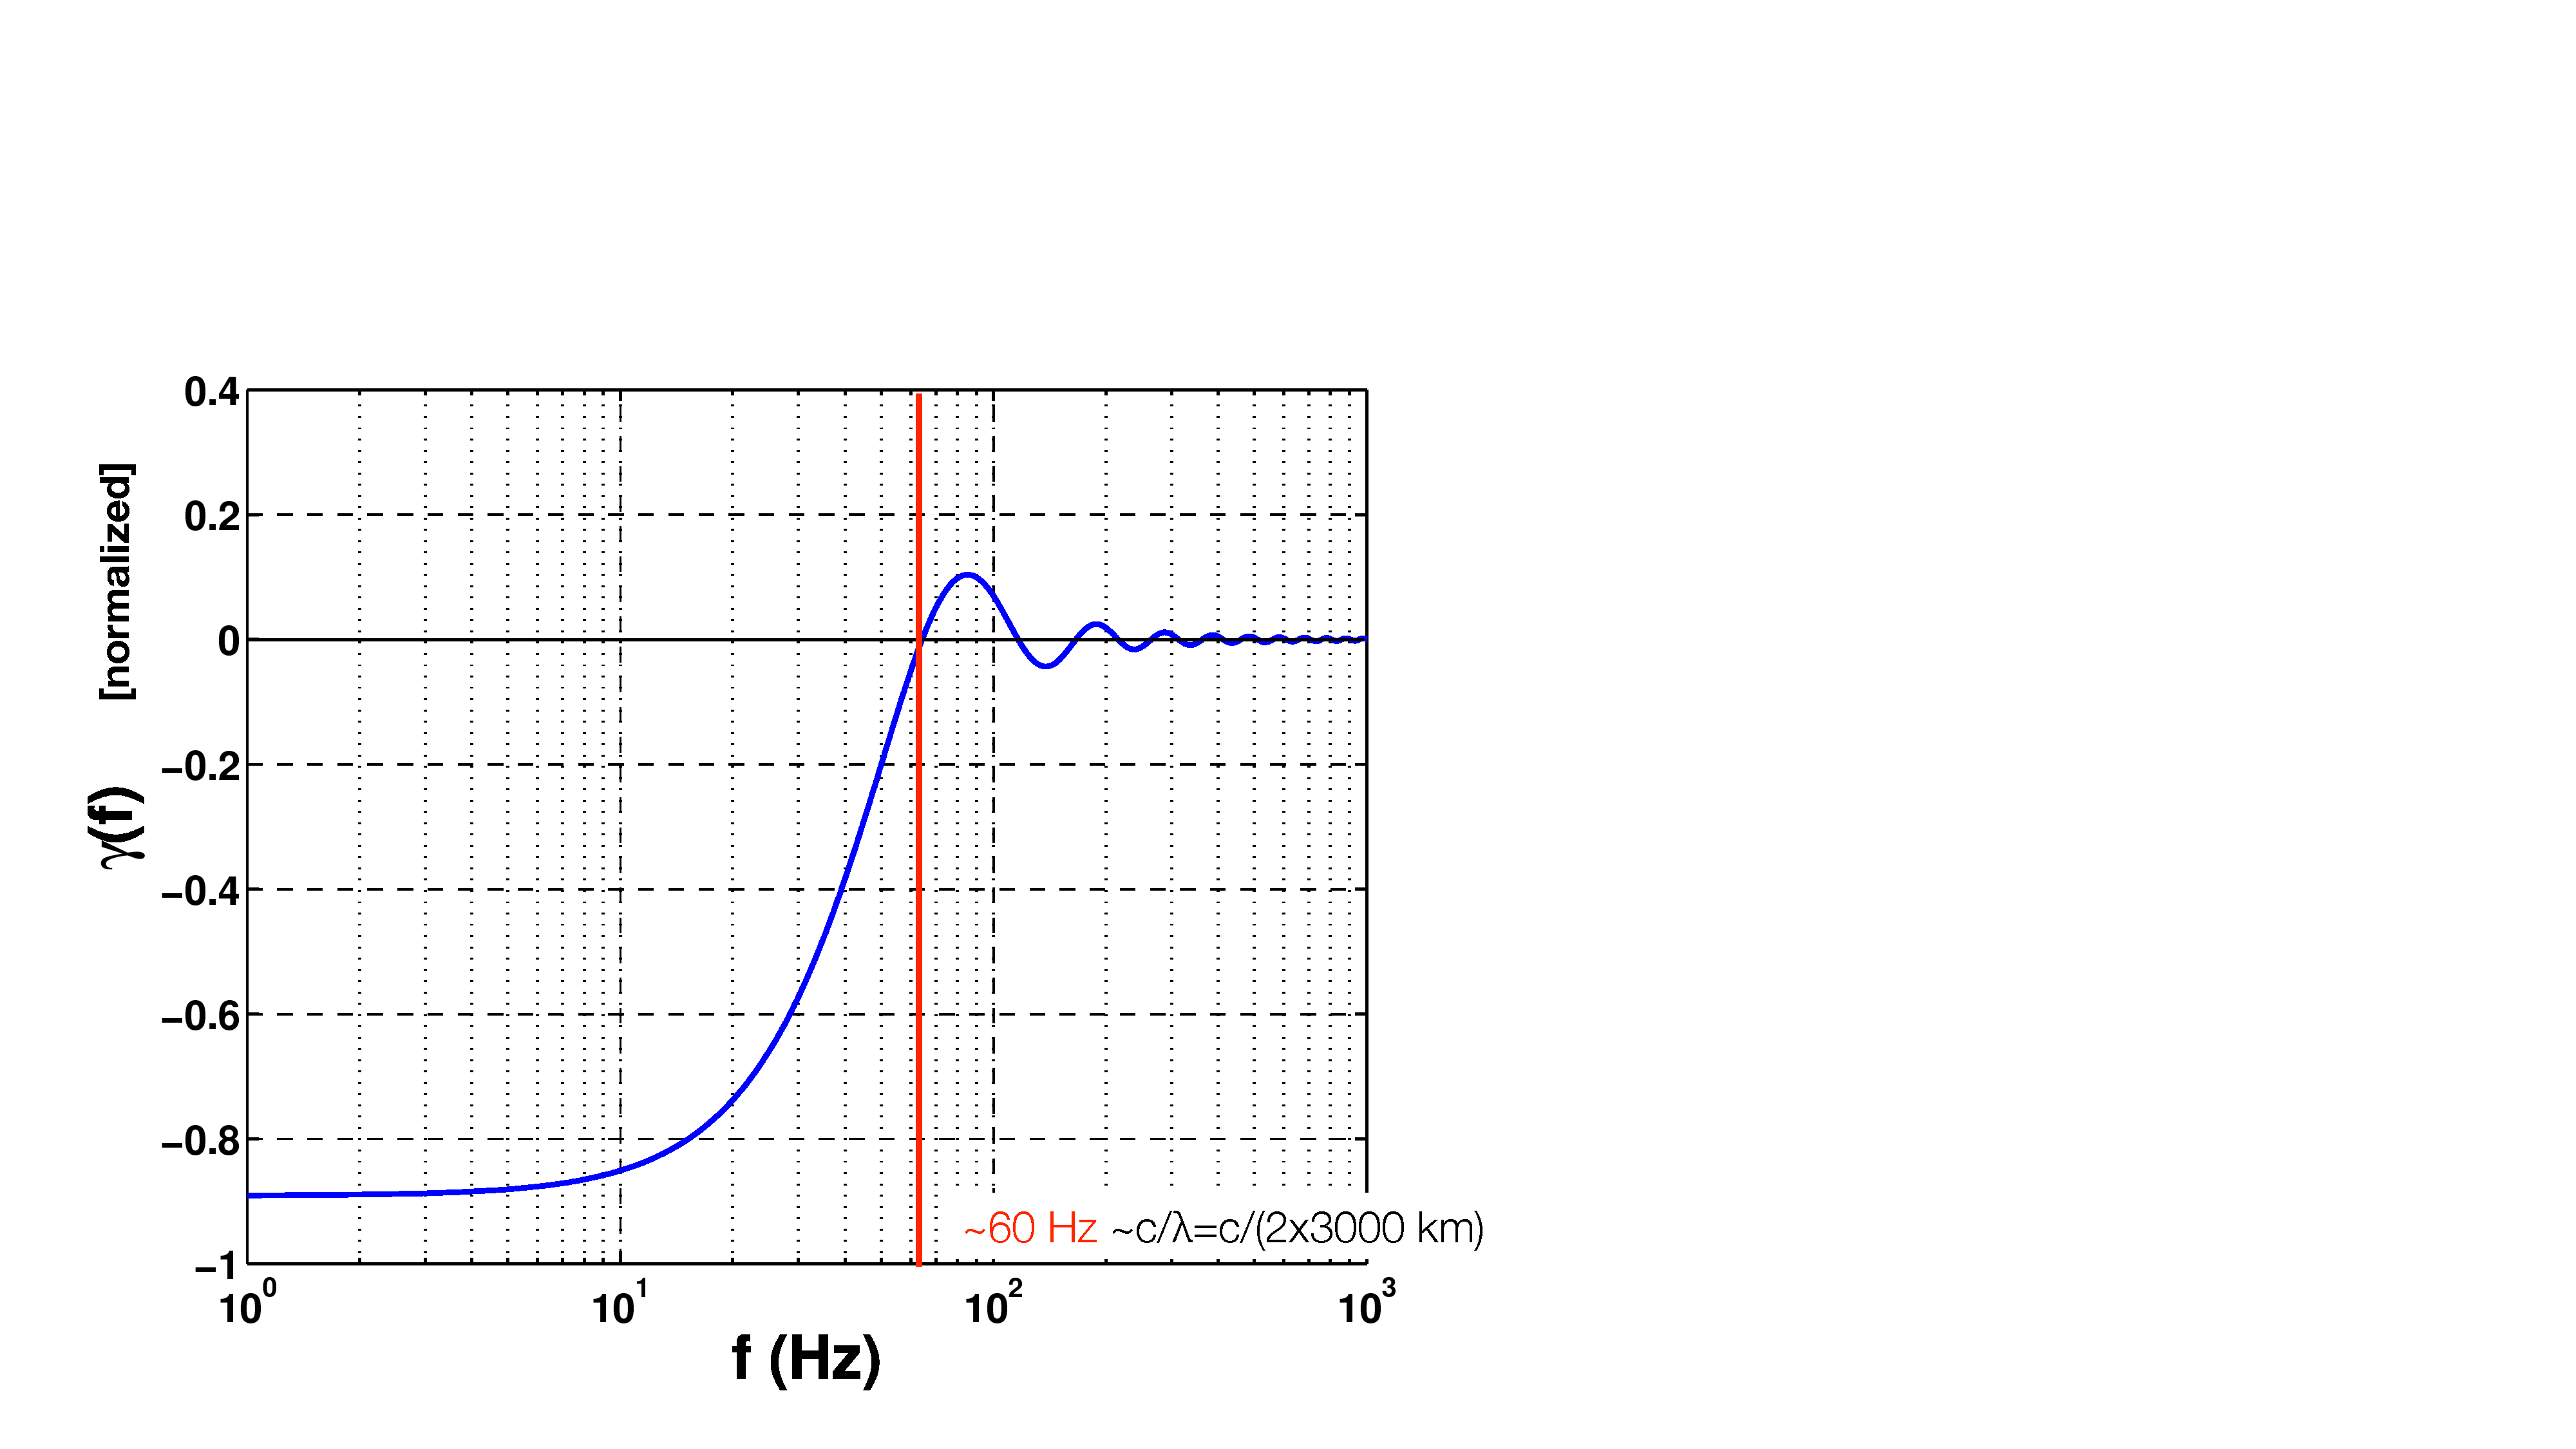
\includegraphics[width=0.49\textwidth]{Figures/LHO-LLO-orf}
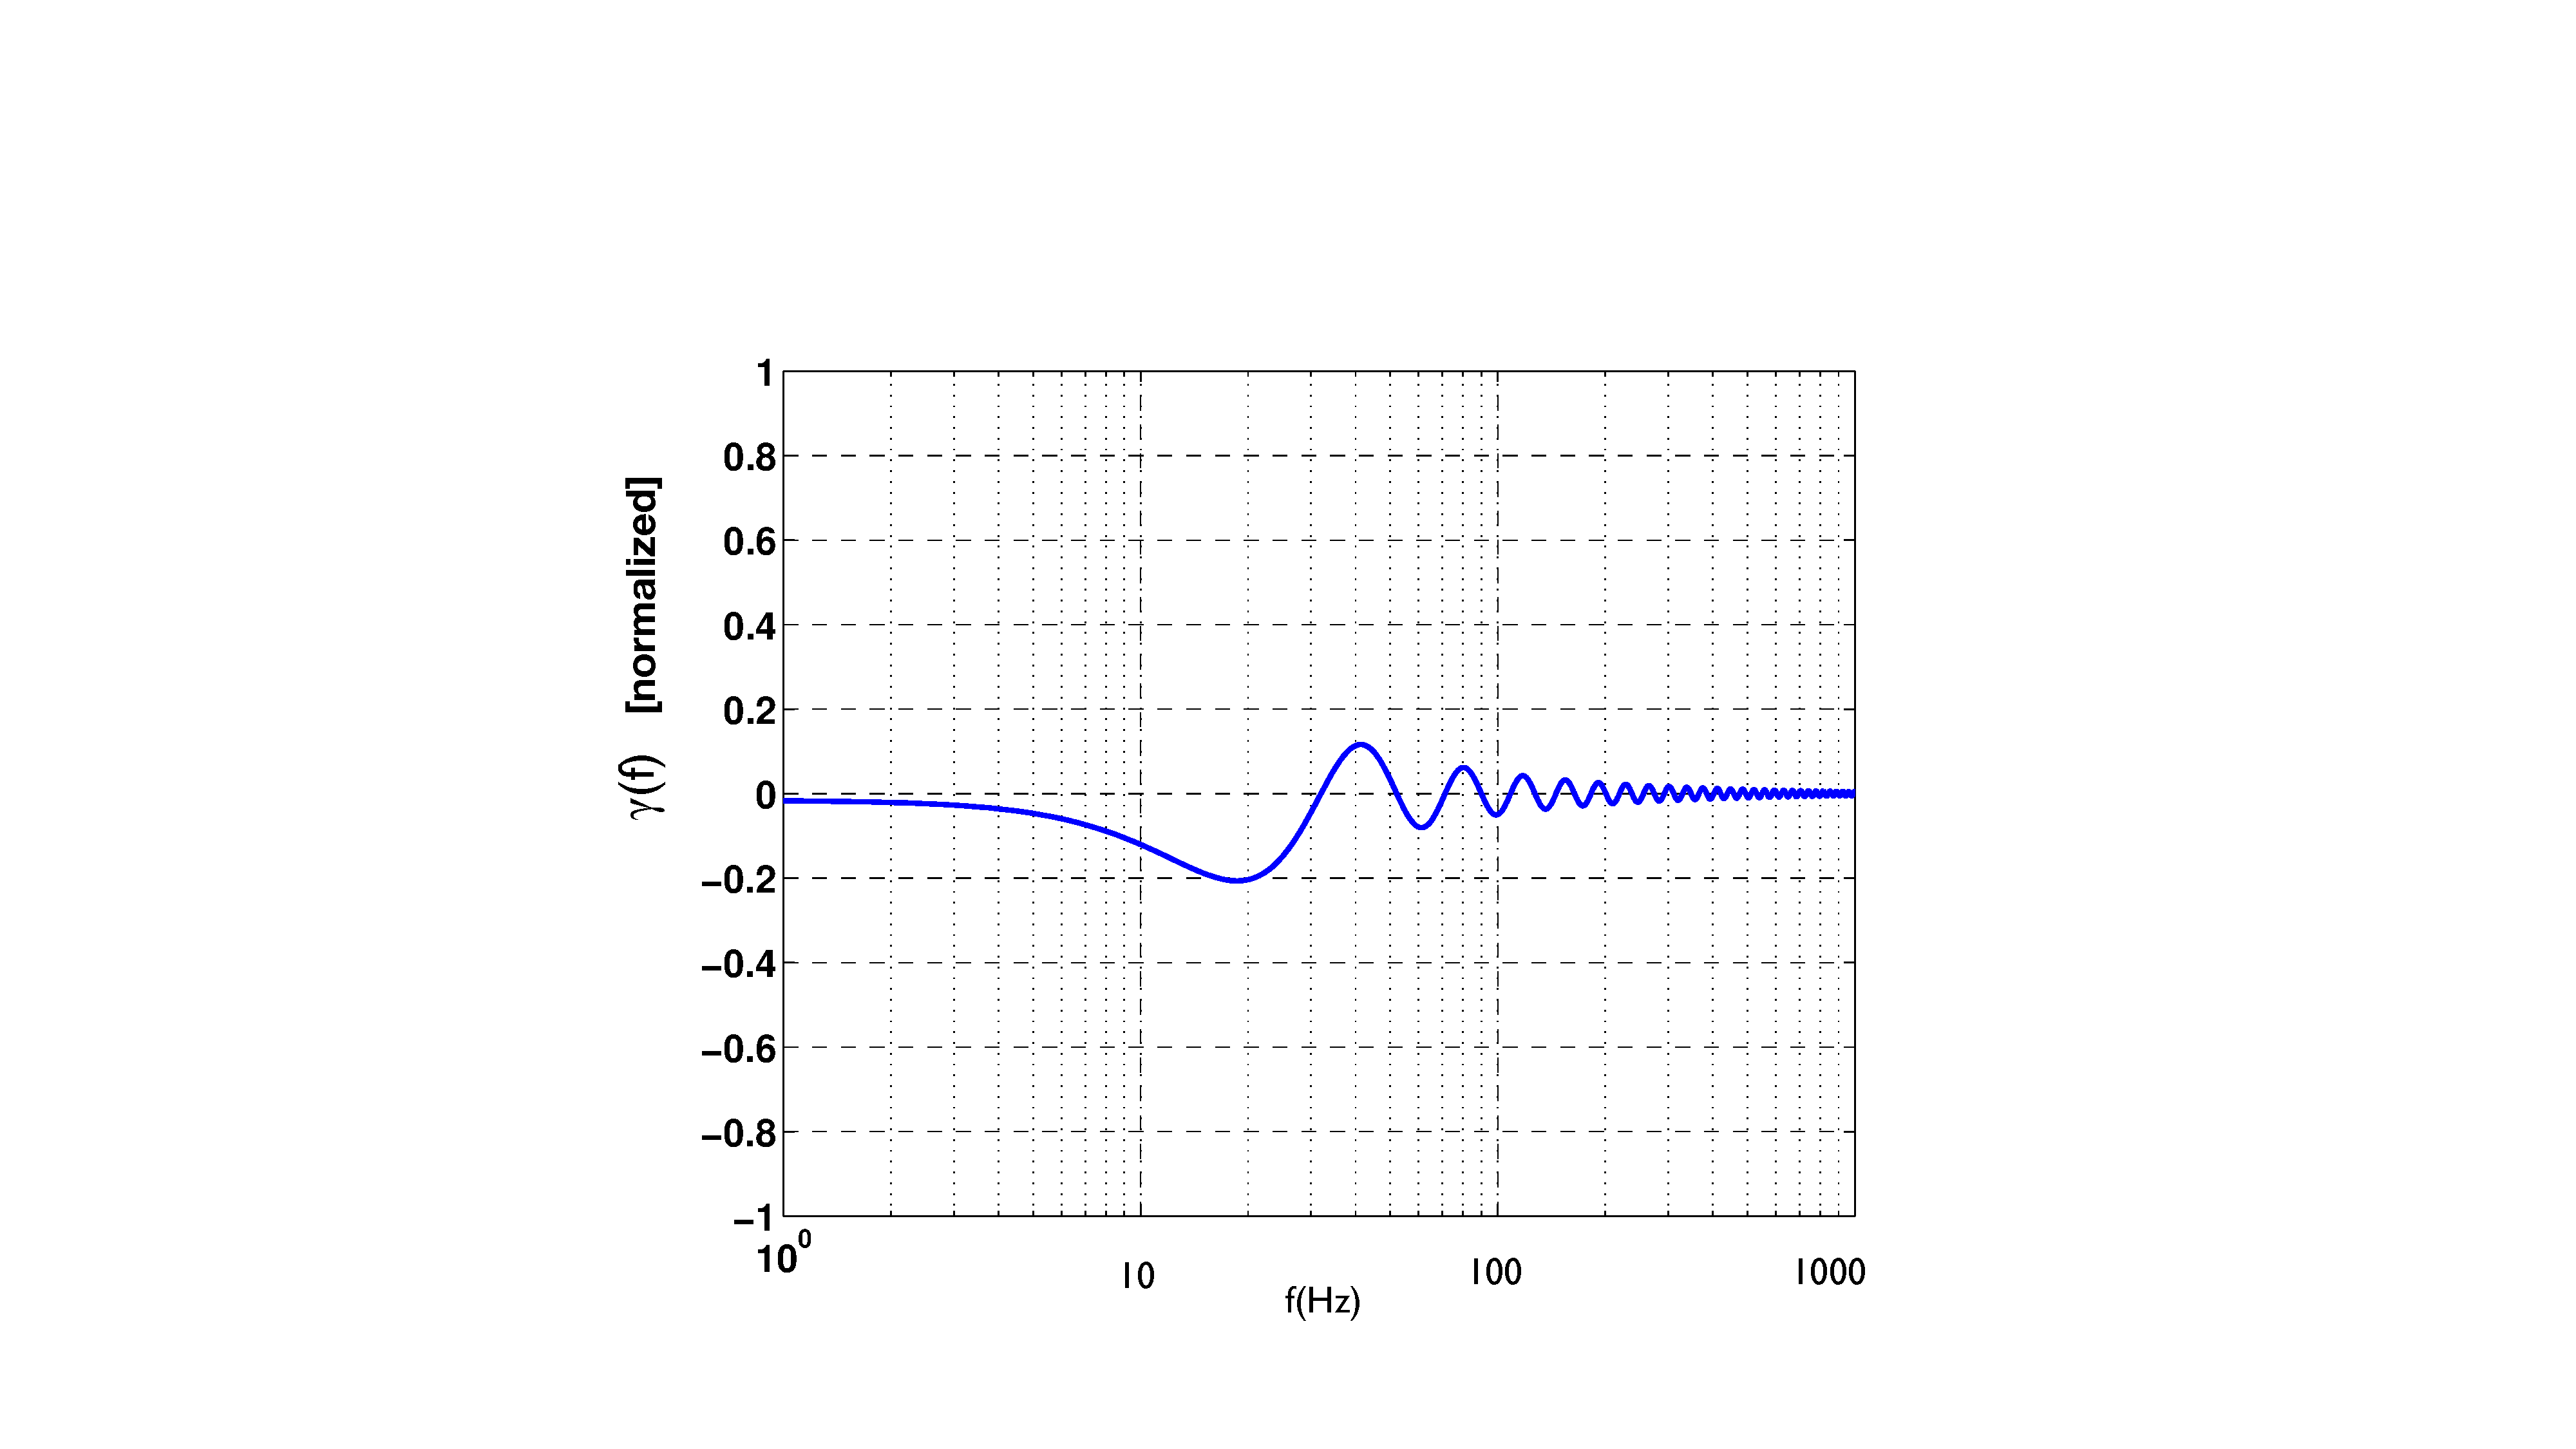
\includegraphics[width=0.49\textwidth]{Figures/LHO-Virgo-orf}
\caption{Normalized overlap function for ground-based
interferometers calculated in the short-antenna approximation.
Left panel: LHO-LLO overlap funtion.
Right panel: LHO-Virgo overlap function.}
\label{f:orfs}
\end{center}
\end{figure}

For the LHO-LLO detector pair,
note that as $f\rightarrow 0$, $\gamma(f)\rightarrow -0.89$.
The minus sign indicates that the two interferometers
are rotated by $90^\circ$ relative to one another.
The fact that the absolute value $|\gamma(0)|=0.89$ is 
not exactly equal to 1, even though the overlap function
is normalized, indicates that the two interferometers
aren't exactly (anti) aligned.
The two interferometers are separated by $27.2^\circ$ as 
seen from the center of the Earth, so the tangent planes 
of the interferometers are tilted relative to one another due 
to the curvature of the Earth.
In addition, the first zero crossing of the overlap function
occurs at approximately 60~Hz, which corresponds (roughly)
to the frequency (50~Hz) of a GW having a wavelength 
equal to 
twice the separation ($2\times 3000$~km) between the two observatories.
For lower frequencies, the two interferometers are driven
(on average) by the same positive (or negative) part of a passing GW;
while for slightly larger frequencies, the two interferometers 
start to be driven by parts of the GW having opposite signs.  
The zero crossings correspond to the transitions between
these in-phase and out-of-phase excitations of the 
interferometers.

For the LHO-Virgo detector pair, note 
that in the limit $f\rightarrow 0$, $\gamma(f)\simeq 0$.
This is because the two interferometers effectively respond
to the two orthogonal polarizations of a GW, corresponding 
to a rotation by $45^\circ$.
This $45^\circ$ misalignment is also the reason for the 
(overall) reduced amplitude of the LHO-Virgo overlap 
function relative to that for LHO-LLO.  
The fact that the first zero crossing for the LHO-Virgo 
overlap function is just over $30^\circ$ (almost half of 
that for LHO-LLO) is due the larger separation between the
LHO and Virgo interferometers, compared to that for LHO 
and LLO.

\subsubsection{Overlap function for pulsar timing arrays}

If one uses \eqref{e:F^A(k)} for the Doppler frequency
repsonse of a pulsar timing measurement, then the correlation
between two Earth-pulsar baselines is just a single number as 
the response functions $F^A_{I,J}(\hat k)$ are independent of
frequency.
This number, which can be interpreted as the expected
correlation between the two pulsar timing measurements, 
depends on the angular separation between the two 
Earth-pulsar baselines:
%
\be
\chi(\zeta_{IJ})\equiv
\frac{1}{2} + \frac{3}{2}\left(\frac{1-\cos\zeta_{IJ}}{2}\right)
\left[\ln\left(\frac{1-\cos\zeta_{IJ}}{2}\right) - \frac{1}{6}\right]
+\frac{1}{2}\,\delta_{IJ}\,,
\label{e:HD}
\ee
%
where $\zeta_{IJ} = \cos^{-1}(\hat p_I\cdot\hat p_J)$, with 
$\hat p_{I,J}$ being unit vectors pointing in the directions
to the pulsars ($\hat p=-\hat u$ in the notation 
of \eqref{e:F^A(k)}).
A plot of this expected correlation as a function of the 
angular separation between the Earth-pulsar baselines is
shown in Figure~\ref{f:HD_curve}.
%
\begin{figure}[htbp!]
\begin{center}
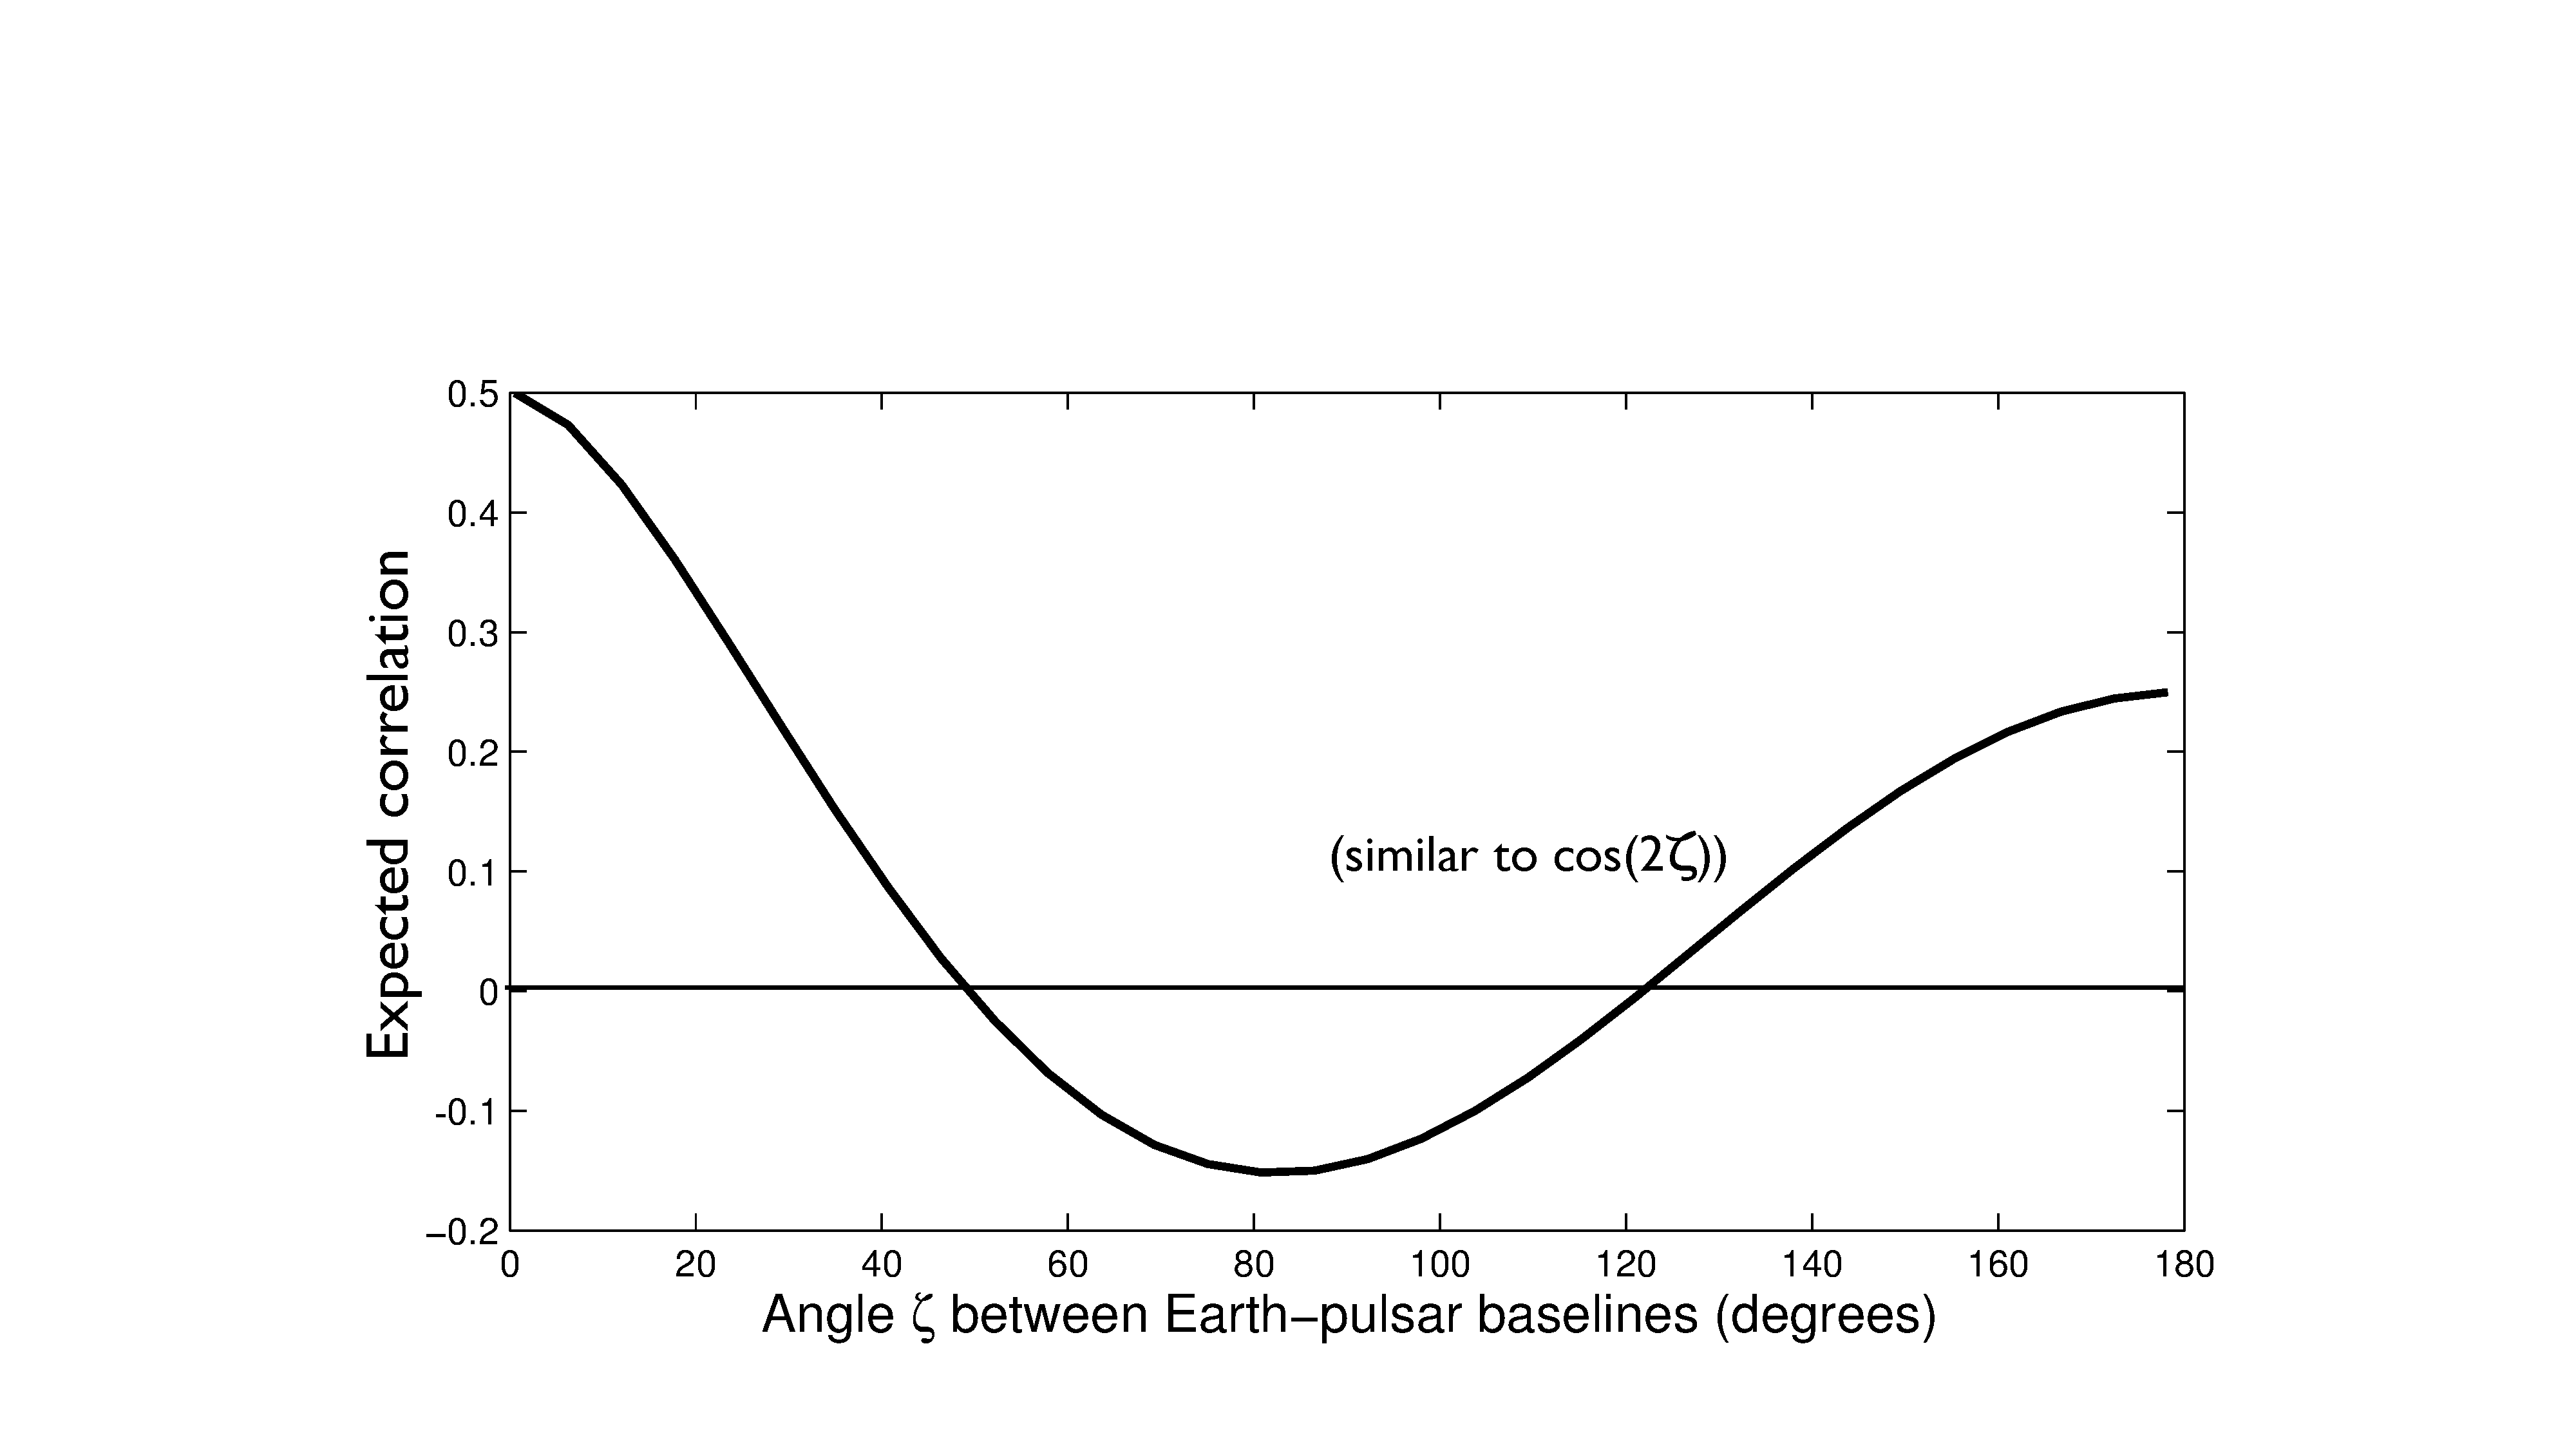
\includegraphics[width=0.7\textwidth]{Figures/HD_curve}
\caption{Hellings-Downs curve.
The values of the expected correlation for an unpolarized,
isotropic GWB as a function of the angle $\zeta$ between
two Earth-pulsar baselines.}
\label{f:HD_curve}
\end{center}
\end{figure}
%
This is called the {\em Hellings-Downs curve}, originally 
calculated in 1983 by Hellings and Downs~\cite{Hellings-Downs:1983}.
This calculation assumes that the GWB is unpolarized
and isotropic.
Generalizations of the Hellings-Downs curve allowing for 
anisotropy and non-general-relativity polarization modes
can be found in e.g., \cite{Mingarelli-et-al, Lee-et-al}.
The quadrupolar nature of GWs in general relativity is
apparent in the Hellings-Down curve, with an angular dependence
that is qualitatively similar to $\cos(2\zeta)$, where 
$\zeta$ is the angle between two Earth-pulsar baselines.

The fact that $\chi(0^\circ)$ is twice as large as
$\chi(180^\circ)$ can easily be demonstrated by using 
\eqref{e:FA_Earth_z} for the relevant response functions.
Taking the two pulsars to point in the same direction
($\hat p_1=\hat p_2 = \hat z$), we have
%
\be
\sum_A F_1^A(\hat k) F_2^A(\hat k) = \frac{1}{4}(1+\cos\theta)^2\,,
\ee
%
while having them point in opposite directions
($\hat p_1 = -\hat p_2=\hat z$) leads to
%
\be
\sum_A F_1^A(\hat k) F_2^A(\hat k) = \frac{1}{4}(1+\cos\theta)(1-\cos\theta)
= \frac{1}{4}\sin^2\theta\,.
\ee
%
These functions are plotted in Figure~\ref{f:pulsar_overlap},
where $\theta$ is the usual polar angle measured with respect
to the $z$-axis.
Multiplying by $1/8\pi$ and integrating 
over the sphere, we find:
%
\be
\Gamma_{12} = \frac{1}{6}\quad({\rm for}\ \hat p_1=\hat p_2=\hat z)\,,
\qquad
\Gamma_{12} = \frac{1}{12}\quad({\rm for}\ \hat p_1=-\hat p_2=\hat z)\,.
\ee
%
The factor of 3 difference between these values and $\chi(0^\circ)=1/2$
and $\chi(180^\circ)=1/4$ is due to a normalization factor that is conventionally
applied to relate $\Gamma_{IJ}$ to $\chi(\zeta_{IJ})$.
From Figure~\ref{f:pulsar_overlap}, we see that when the 
two pulsars both point in the $\hat z$ direction, 
the majority of support for the overlap function comes from 
sky directions $\hat n=-\hat k$ having $z>0$.
When the two pulsars point in opposite directions, 
$\hat p_1=-\hat p_2=\hat z$,
the majority of support for the overlap function comes 
from sky directions in the $xy$-plane, which is
a smaller contribution.
%
\begin{figure}[htbp!]
\begin{center}
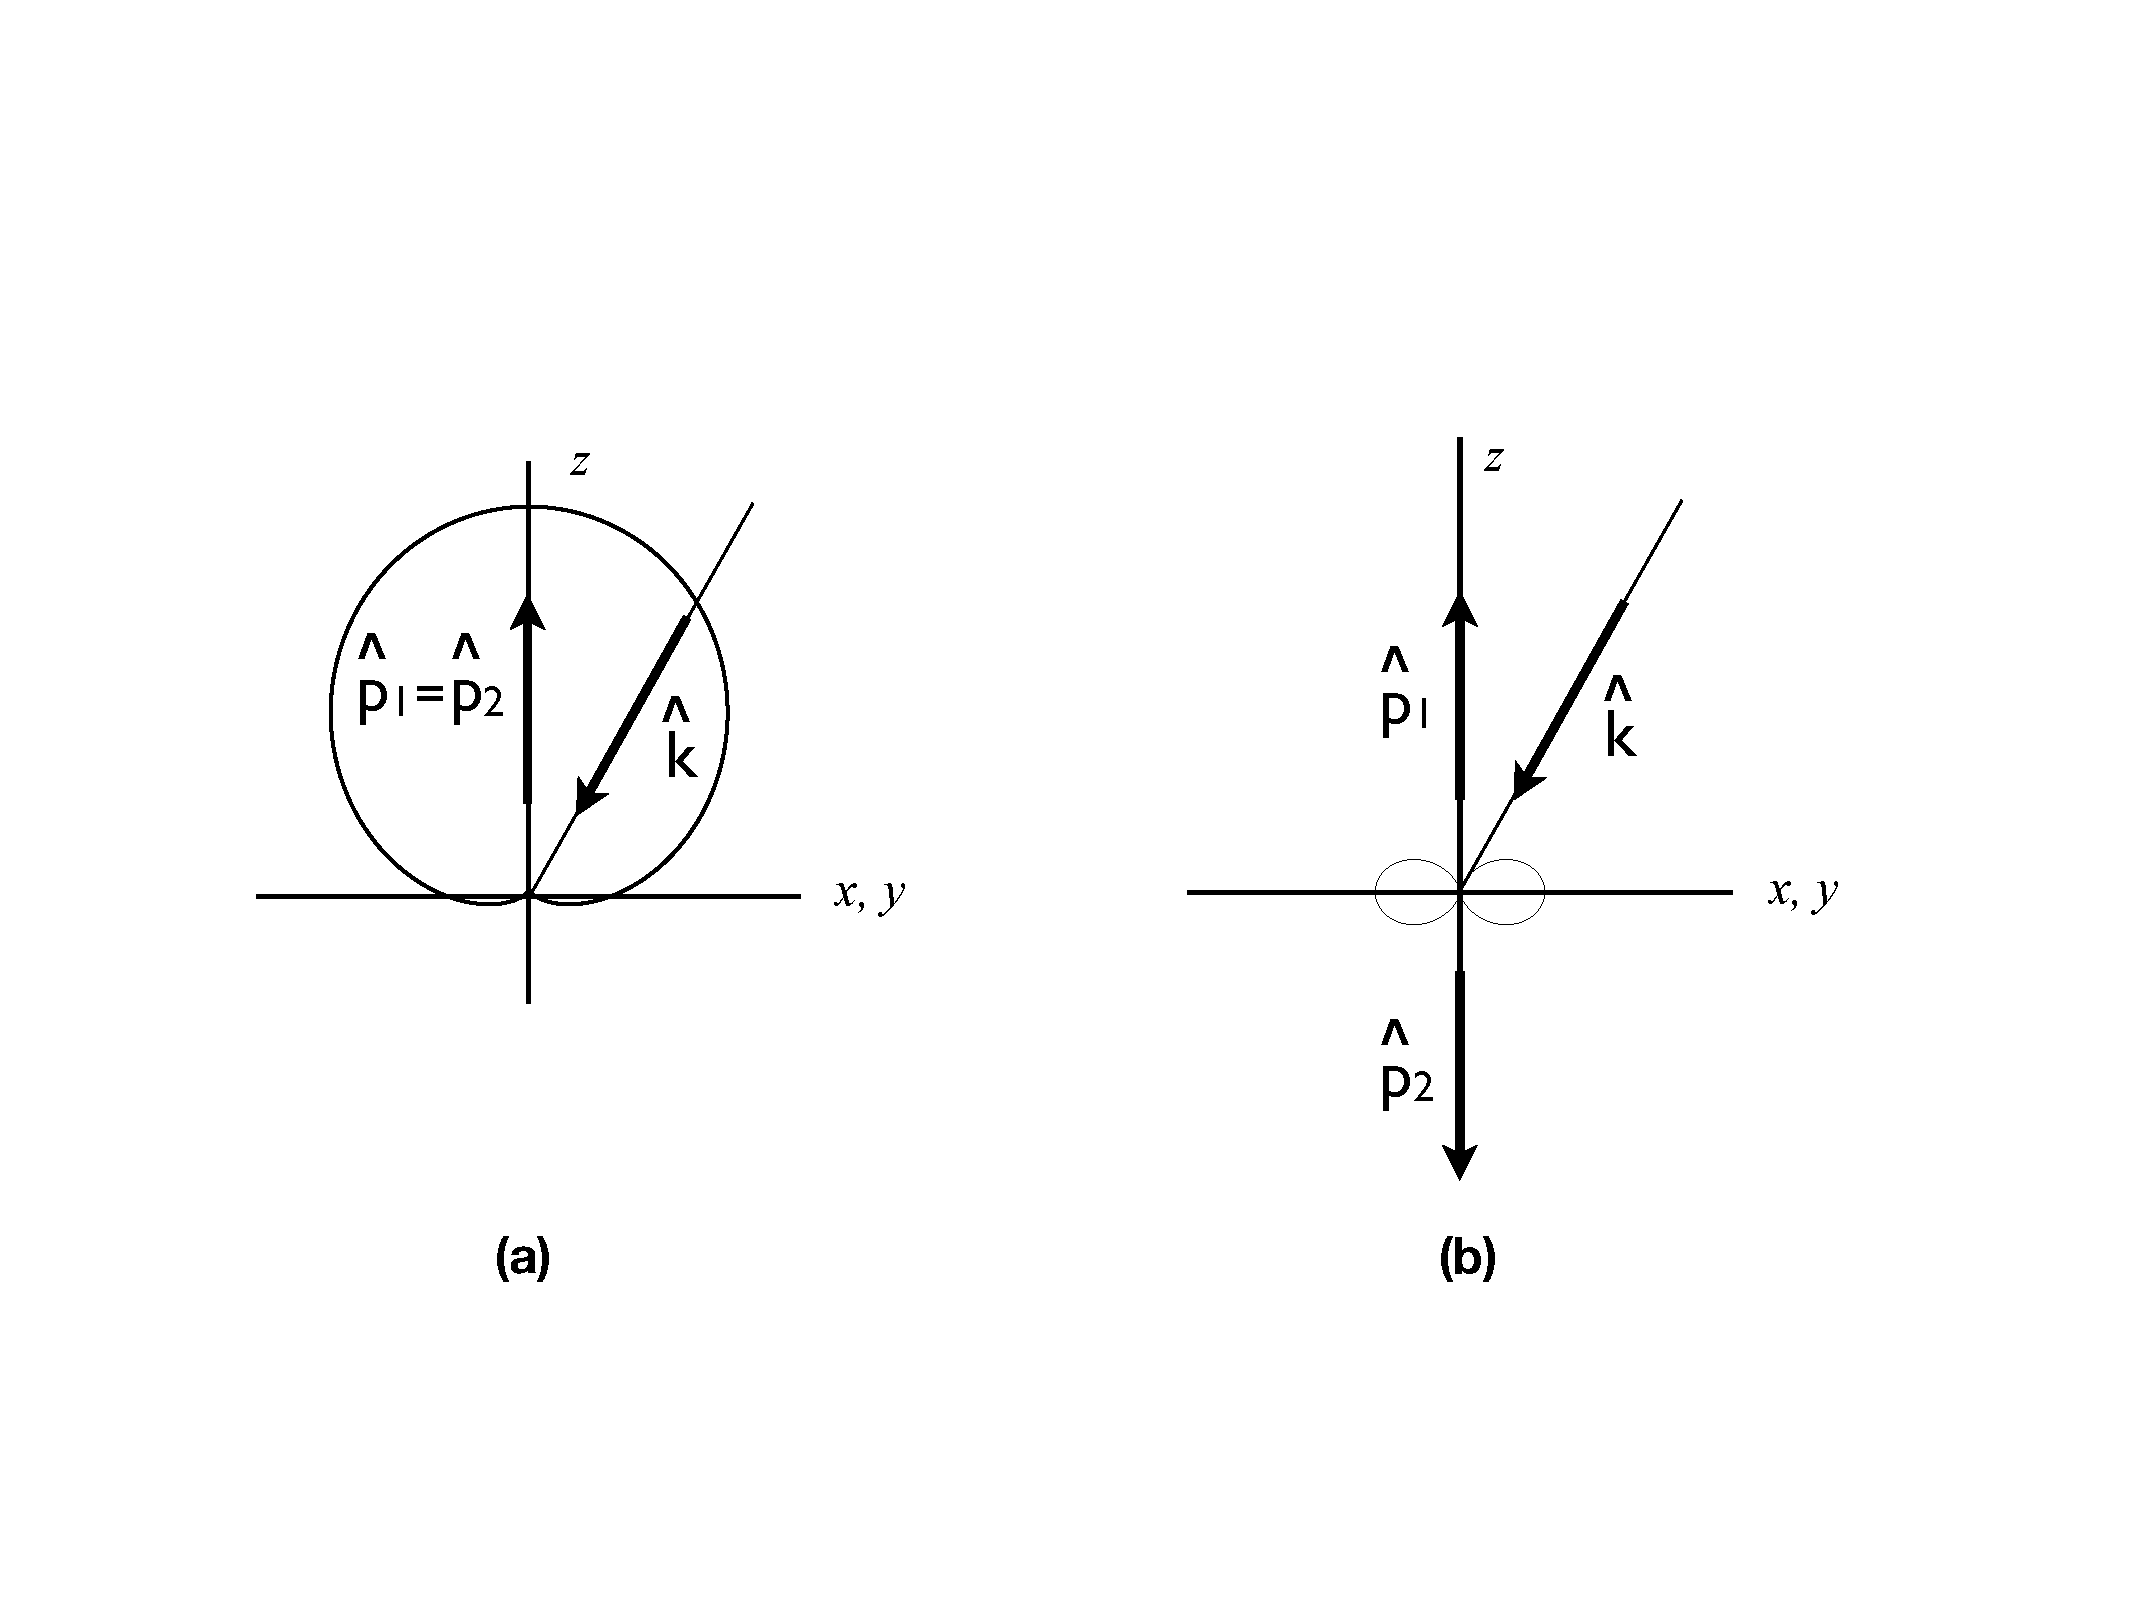
\includegraphics[width=0.8\textwidth]{Figures/pulsar_overlap}
\caption{Graphical representation of the integrand of the 
(Earth-only) overlap function for pulsar timing Doppler frequency
measurements.
Panel (a): integrand for two Earth-pulsar baselines having
$\zeta = 0^\circ$ ($\hat p_1=\hat p_2=\hat z)$;
Panel (b): integrand for two Earth-pulsar baselines having
$\zeta = 180^\circ$ ($\hat p_1=-\hat p_2 =\hat z)$.
These functions are axially symmetric around the $z$-axis,
which we've chosen to be the direction to pulsar 1.}
\label{f:pulsar_overlap}
\end{center}
\end{figure}
%

\subsubsection{Overlap function for a pair of electric dipole 
antennae}

For the final example, you are asked in Exercise~\ref{exer:7} to 
calculate the overlap function for a pair of short, colocated
electric dipole antennae in the presence of an unpolarized
and isotropic electric field $\vec E(t,\vec x)$.
The two dipole antennae point in different directions
separated by an angle $\zeta$ as shown in Figure~\ref{f:dipole-orf}.
%
\begin{figure}[htbp!]
\begin{center}
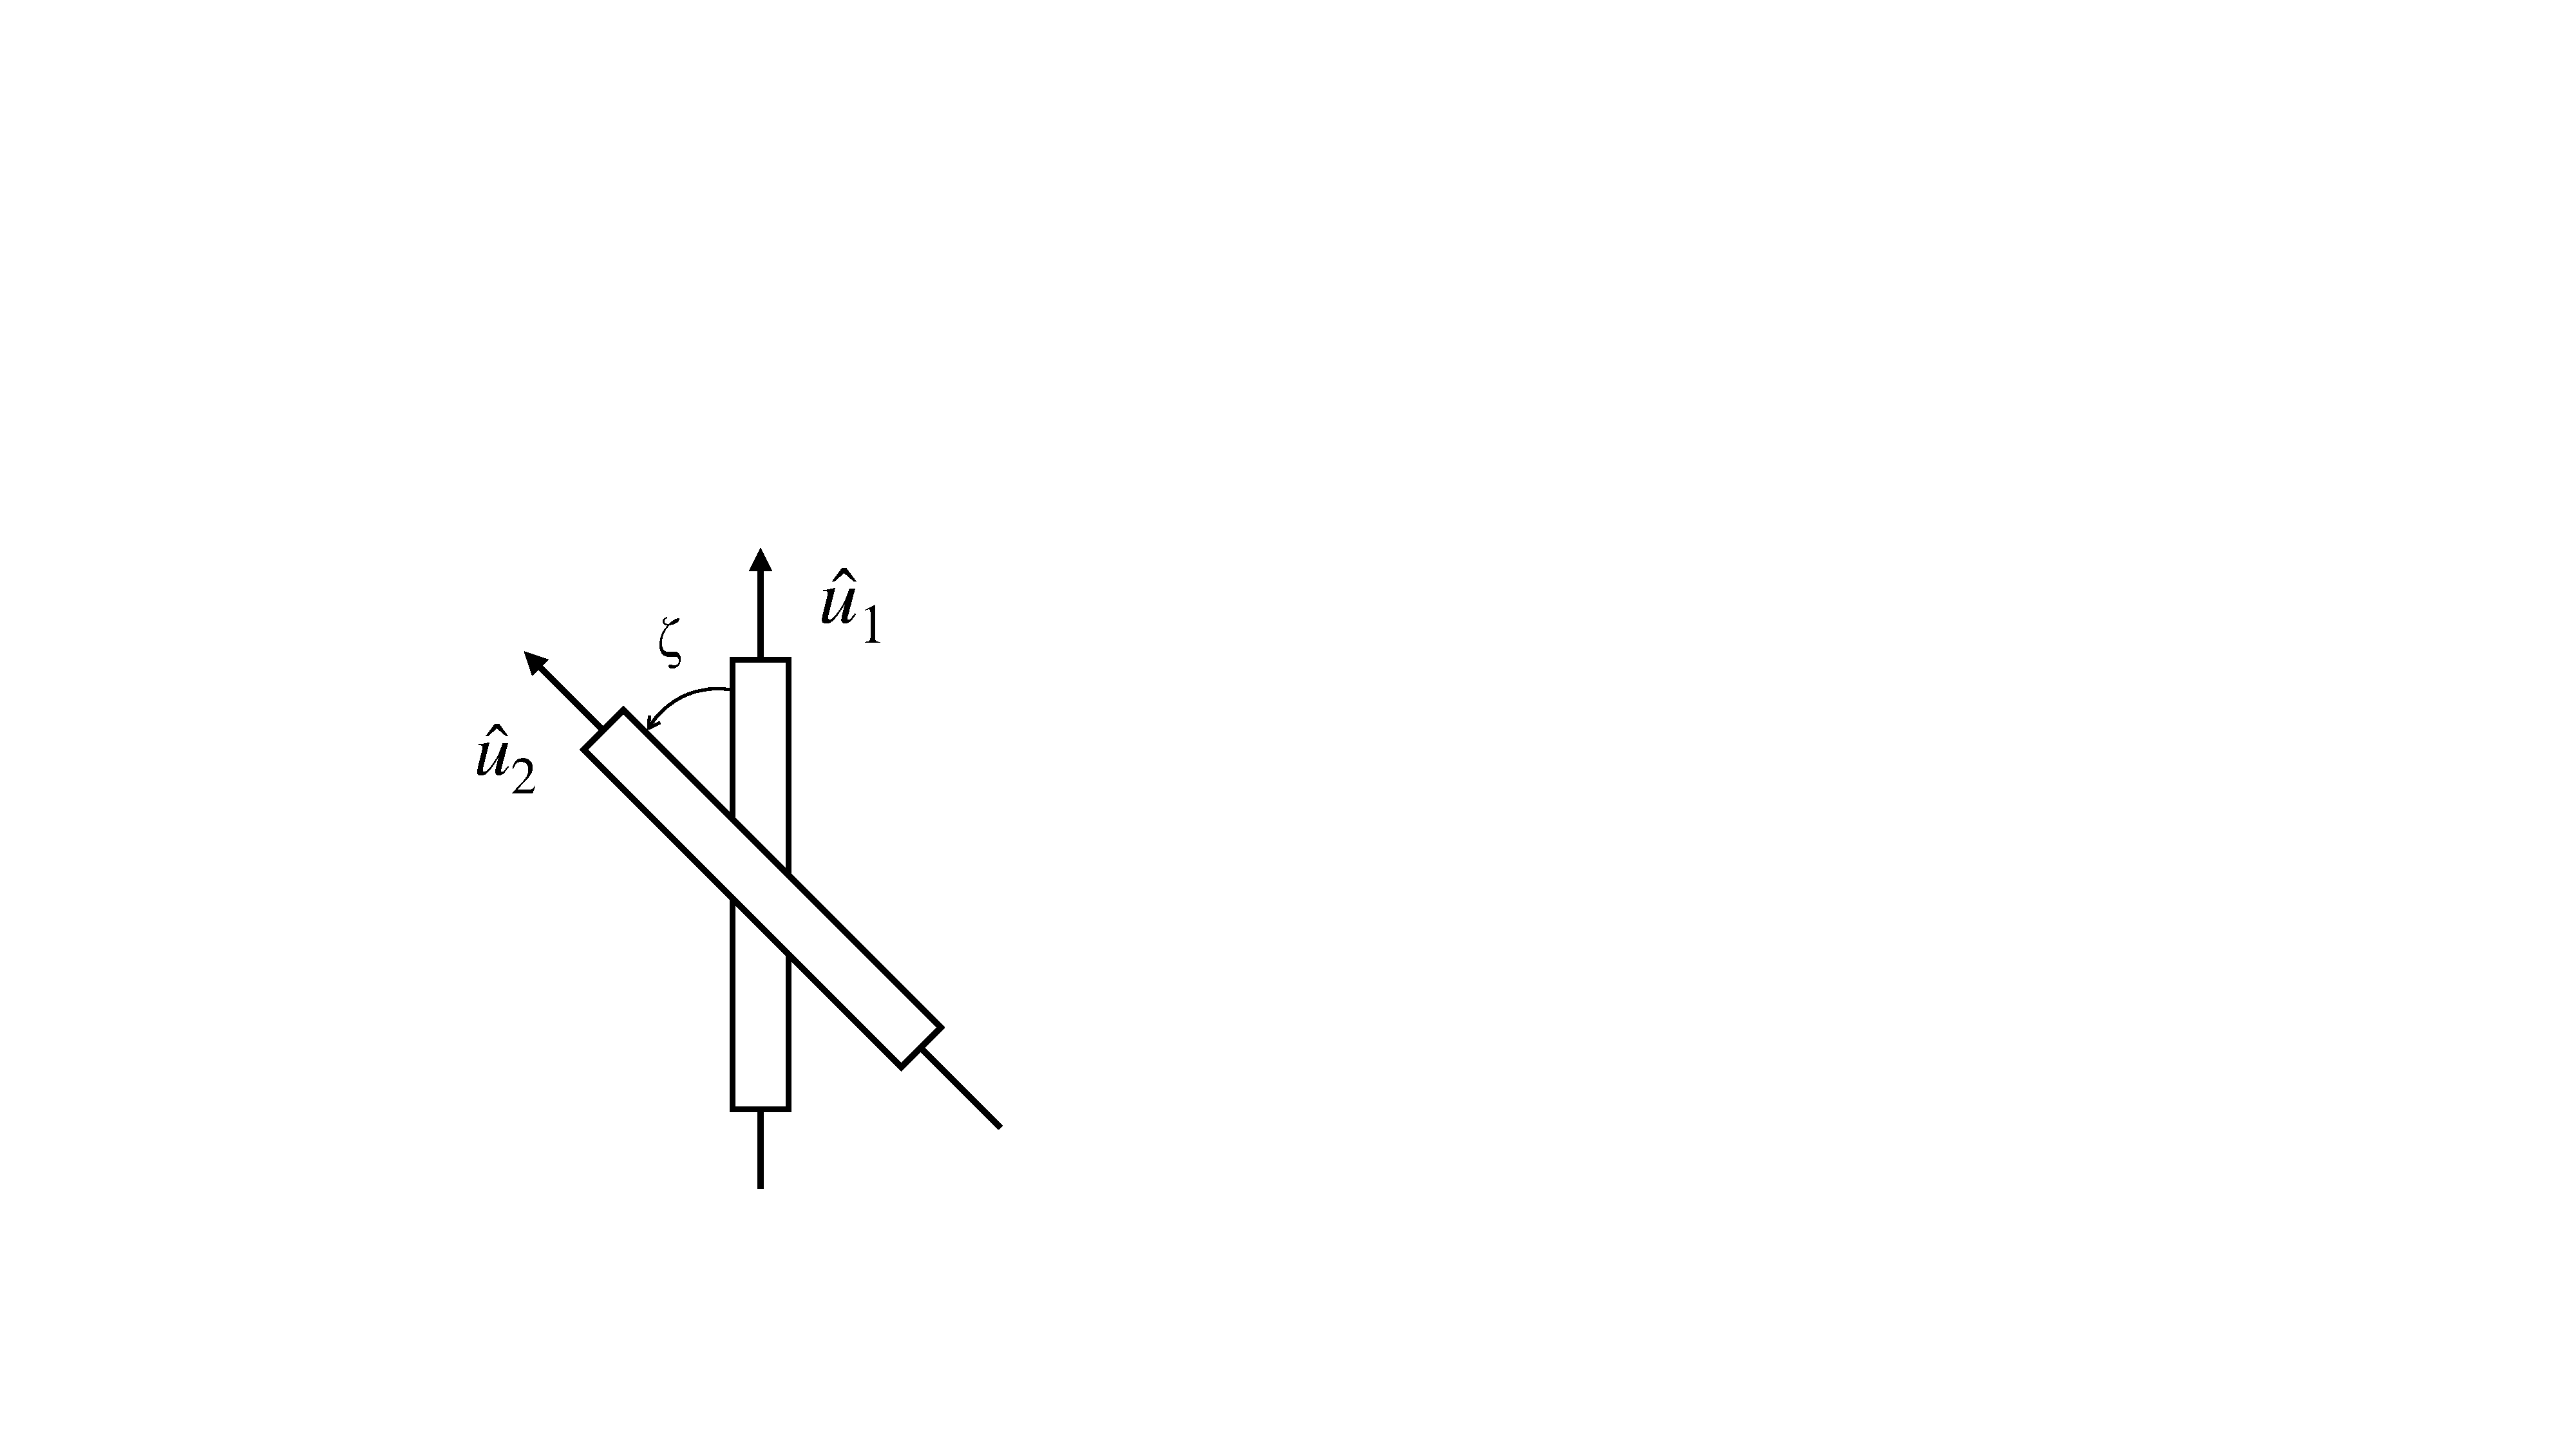
\includegraphics[width=0.25\textwidth]{Figures/dipole-orf}
\caption{Geometry for calculating the overlap function
for a pair of short, colocated electric dipole antennae, 
for an unpolarized and isotropic electric field
(Exercise \ref{exer:7}).}
\label{f:dipole-orf}
\end{center}
\end{figure}
%
To do the calculation, you should use the fact that the 
response of dipole $I$ to the electric field is 
%
\be
r_I(t) = \hat u_I\cdot\vec E(t,\vec x_0)\,.
\ee
%
The electric field can be expanded in a manner
similar to that for an unpolarized, isotropic GWB:
%
\be
\vec E(t,\vec x) = \int_{-\infty}^\infty df\>\int d^2\Omega_{\hat k}\> 
\sum_{\alpha =1}^2 \tilde E_\alpha(f,\hat k)\hat\epsilon_\alpha(\hat k) 
e^{i2\pi f(t-\hat k\cdot \vec x/c)}
\ee
%
where the polarization vectors are given by
%
\be
\hat\epsilon_1(\hat k) = \hat \theta\,,
\quad
\hat\epsilon_2(\hat k) = \hat \phi\,.
\ee
%
In addition, the Fourier components $\tilde E_\alpha(f,\hat k)$
satify the quadratic expectation values, cf.~\eqref{e:quad_iso}:
%
\be
\langle \tilde E_\alpha(f,\vec k) \tilde E_{\alpha'}^*(f',\hat k')\rangle
=\frac{1}{16\pi} S_E(f)\delta(f-f')\delta_{\alpha\alpha'}
\delta^2(\hat k,\hat k')\,.
\ee
%
With these definitions, it is then just a matter of 
``turning the crank" to calculate
the expectation value $\langle r_1(t) r_2(t')\rangle$, from
which you can read off the overlap function $\Gamma_{12}(f)$,
see~\eqref{e:Gamma-time}.
You should find
%
\be
\Gamma_{12}(f) =\frac{2}{3}\,\hat u_1\cdot\hat u_2 
=\frac{2}{3}\cos\zeta\,.
\ee
%
The dipole nature of the antennae shows up in the $\cos\zeta$ 
dependence of the overlap function.

%%%%%%%%%%%%%%%%%%%%%%%%%%%%%%%%%%%%%%%%%%%%%%%%%%%%%%%
\section{Statistical inference}
\label{s:statistical_inference}

In order to discuss our final example (Section~\ref{s:nonstationary}),
which is an optimal search for the popcorn-like background
produced by stellar-mass BBH mergers throughout the 
universe, we need to go beyond the frequentist 
statistics that we have used so far 
(Section~\ref{s:correlations}), 
and introduce some concepts from the field of Bayesian inference.
So here, we briefly introduce Bayesian inference by comparing 
it to frequentist statistics, focusing mainly on those topics 
needed for the stochastic search that we shall describe in
Section~\ref{s:nonstationary}.
Readers who are interested in more details should 
consult John Veitch's contribution to this Volume.

\subsection{Comparing frequentist statistics and Bayesian inference}

We start by listing the key ingredients of these two formulations 
of statistical inference.
\medskip

\noindent{Frequentist statistics:}

\bi

\i probabilities are long-run relative occurrence of 
outcomes of repeatable experiments (i.e., random variables);
probabilities cannot be assigned to hypotheses or parameters, 
which have fixed but unknown values.

\i one usually starts by writing down a likelihood 
function $p(d|H)$, which is the probability distribution 
for the measured data $d$, assuming the truth of a particular
hypothesis $H$.

\i to estimate the value of parameters and/or to decide
between different hypotheses, one constructs 
{\em statistics}, which are particular functions of the data.

\i to make probabilistic statements about 
parameter estimates or hypothesis testing, 
one needs to calculate
the probability distributions of the statistics;
this can be done either analytically or numerically 
(e.g., using time slides).

\i given the probability distributions of the statistics,
one can then construct confidence intervals and 
$p$-values (the probability of obtaining a detection
statistic value as large or larger than what was measured) 
for parameter estimation and hypothesis testing.

\ei

\noindent{Bayesian inference:}

\bi

\i probability is degree of belief (or confidence)
in any proposition, and hence can be assigned to 
hypotheses and parameters.
(This is a more general definition of probability than 
that used in frequentist statististics.)

\i like a frequentist, one usually starts by writing 
down a likelihood function $p(d|H)$.

\i in addition to the likeihood function, one needs to
specify prior probability distributions for the various 
parameters and hypotheses that one is considering.

\i one uses Bayes' theorem to update the prior degree 
of belief in a parameter value or hypothesis in light 
of new data.

\i one constructs posterior distributions and odds 
ratios (or {\em Bayes factors}, see Section~\ref{s:bayes_factors}) 
for parameter estimation and hypothesis testing (also 
called model selection).

\ei
\noindent
In a nutshell, the main different between Bayesian and 
frequentist statistics is the definition of probability.
As such, certain probabilistic statements that you can
make as a Bayesian are not valid from a frequentist perspective.
Hence Bayesian and frequentist statistic often ask 
(and subsequently answer) {\em different} questions 
about the data.
Nonetheless, despite this fundamental difference in approach,
if the data are sufficiently informative (i.e., if the 
likelihood is peaked relative to the prior distributions 
for the parameters, see Figure~\ref{f:informative_data}), 
then both Bayesian and frequentist analyses give more or 
less consistent results.

\subsubsection{Likelihood functions}
\label{s:likelihood}

As mentioned above, the starting point for most 
frequentist and Bayesian analyses is a likelihood function,
which we can write schematically as
%
\be
{\rm likelihood} = p({\rm data}| {\rm parameters}, {\rm model})\,.
\ee
%
For example, for Gaussian-distributed detector noise 
and a Gaussian-distributed GWB, the likelihood 
function for the noise-only model ${\cal M}_0$ and 
signal+noise model ${\cal M}_1$ are given by
%
\begin{align}
&p(d|S_{n_1}, S_{n_2}, {\cal M}_0) 
= \frac{1}{\sqrt{{\rm det}(2\pi C_n)}}\, 
\exp\left[-\frac{1}{2} d^T C_n^{-1} d\right]\,,
\label{e:noise_likelihood}
\\
&p(d|S_{n_1}, S_{n_2}, S_h, {\cal M}_1) 
= \frac{1}{\sqrt{{\rm det}(2\pi C)}}\, 
\exp\left[-\frac{1}{2} d^T C^{-1} d\right]\,,
\label{e:stochastic_likelihood}
\end{align}
%
where $C_n$ and $C$ are the covariance matrices
for the noise-only and signal+noise models, respectively.
For $N$ samples of white noise and white GWB in
two colocated and coaligned detectors:
%
\be
C_n = \begin{bmatrix}
S_{n_1}\,{\mathsf 1}_{N\times N} & {\mathsf 0}_{N\times N}\\
{\mathsf 0}_{N\times N} & S_{n_2}\,{\mathsf 1}_{N\times N}
\end{bmatrix}
\quad\&\quad
C = \begin{bmatrix}
(S_{n_1} + S_h)\,{\mathsf 1}_{N\times N} & S_h\,{\mathsf 1}_{N\times N}\\
S_h\,{\mathsf 1}_{N\times N} & (S_{n_2}+S_h)\,{\mathsf 1}_{N\times N}
\end{bmatrix}\,.
\label{e:covariance_matrices}
\ee
%
For this simple case, there are only three relevant 
parameters: $S_{n_1}$, $S_{n_2}$ for the detector noise, 
and $S_h$ for the GWB.
Also, by assuming that the detectors are colocated and 
coaligned, we don't have to worry about including an 
overlap function in the
off-diagonal blocks of the signal+noise covariance matrix $C$.

\subsection{Frequentist analyses}
\label{s:frequentist}

Starting from the likelihood functions for the noise-only
and signal+noise models, we can construct the 
{\em maximum-likelihood ratio} statistic:
%
\be
\Lambda_{\rm ML}(d)\equiv\frac{
{\rm max}_{S_{n_1},S_{n_2},S_h}\,p(d|S_{n_1} S_{n_2},S_h,{\cal M}_1)}
{{\rm max}_{S_{n_1},S_{n_2}}\,p(d|S_{n_1}, S_{n_2},{\cal M}_0)}\,.
\label{e:Lambda_ML}
\ee
%
The values of the parameters that maximize the likelihood
for the signal+noise model can be used as 
frequentist estimators of the true values of the parameters 
$S_{n_1}$, $S_{n_2}$, $S_h$.
In Exercise~\ref{exer:8} you are asked to show that the 
data combinations
%
\be
\hat C_{11} \equiv 
\frac{1}{N}\sum_{i=1}^N d_{1i}^2\,,
\qquad
\hat C_{22} \equiv 
\frac{1}{N}\sum_{i=1}^N d_{2i}^2\,,
\qquad
\hat C_{12} \equiv 
\frac{1}{N}\sum_{i=1}^N d_{1i}d_{2i}\,,
\ee
% 
are maximum-likelihood estimators of 
%
\be
S_1\equiv S_{n_1}+S_h\,,\quad
S_2\equiv S_{n_2}+S_h\,,\quad
S_h\,.
\ee
%
Note that the maximum-likelihood estimator 
$\hat S_h\equiv \hat C_{12}$ of $S_h$ is just the standard 
cross-correlation statistic introduced in \eqref{e:Sh_ML}.
The maximum-likelihood estimators of the detector
noise $S_{n_1}$, $S_{n_2}$ are then
%
\be
\hat S_{n_1} = 
\hat S_1-\hat S_h=
\hat C_{11}-\hat C_{12}\,,
\qquad
\hat S_{n_2} = 
\hat S_2-\hat S_h=
\hat C_{22}-\hat C_{12}\,.
\ee
%
In addition, in Exercise~\ref{exer:9}, you are asked to 
show that 
%
\be
\Lambda(d)\equiv 2\ln(\Lambda_{\rm ML}(d))
\simeq\frac{\hat C_{12}^2}{\hat C_{11}\hat C_{22}/N}\,,
\label{e:Lambda}
\ee
%
which holds in the {\em weak-signal approximation}, 
where $S_h\ll S_{n_1}, S_{n_2}$.
The quantity $\Lambda(d)$ can be used as a frequentist detection 
statistic, comparing its value for the given data $d$ 
to a threshold $\Lambda_*$.
If $\Lambda(d)\ge \Lambda_*$, we reject the null 
hypothesis (the noise-only model) and claim detection 
of a GW signal; if $\Lambda(d)<\Lambda_*$, we accept
the null-hypothesis and reject the signal+noise hypothesis.
Note that the right-hand-side of \eqref{e:Lambda} is the 
square of the 
(power) signal-to-noise ratio, which illustrates a 
useful general relation between signal-to-noise ratios 
and the maximum-likelihood statisitic.

%%%%%%%%%%%%%%%%%%%%%%%%%%%%%%%%%%%%%%%%%%%%%
\subsection{Bayesian analyses}
\label{s:bayesian}

Not suprisingly, Bayesian analyses make use of Bayes'
theorem:
%
\be
p(H|d) = \frac{p(d|H) p(H)}{p(d)}\,,
\label{e:bayes_theorem}
\ee
%
which converts probabilities about the data $d$ given 
an hypothesis $H$ (the likelihood 
$p(d|H)$) to probabilites about the hypothesis given
the data (the posterior distribution $p(H|d)$).%
\footnote{Conditional probabilities 
$p(A|B)$ and $p(B|A)$ are not equal in general.
Paraphrasing an example from Louis Lyons, 
the probability that a person is pregnant ($A$), 
given that that person is a woman  ($B$) is about 
about 30\%, while the probability that a person is 
a woman ($B$), given that that person is
pregnant ($A$) is 100\%.}
Here, $p(H)$ is the prior probability distribution 
for $H$, and $p(d)$ is the {\em evidence} or 
{\em marginalized likelihood}:
%
\be
p(d) \equiv \int {\rm d}H\>
p(d|H)p(H)\,.
\ee
%
Note that the evidence is simply the normalization 
factor needed to insure $\int {\rm d}H\>p(H|d)=1$.
The importance of Bayes' theorem is that it updates 
our degree of belief in an hypothesis in light
of new data.
It maps the prior probability $p(H)$ to the posterior 
probability $p(H|d)$ via the likelihood function 
$p(d|H)$
(Figure~\ref{f:bayes_theorem}).
%
\begin{figure}[htbp!]
\begin{center}
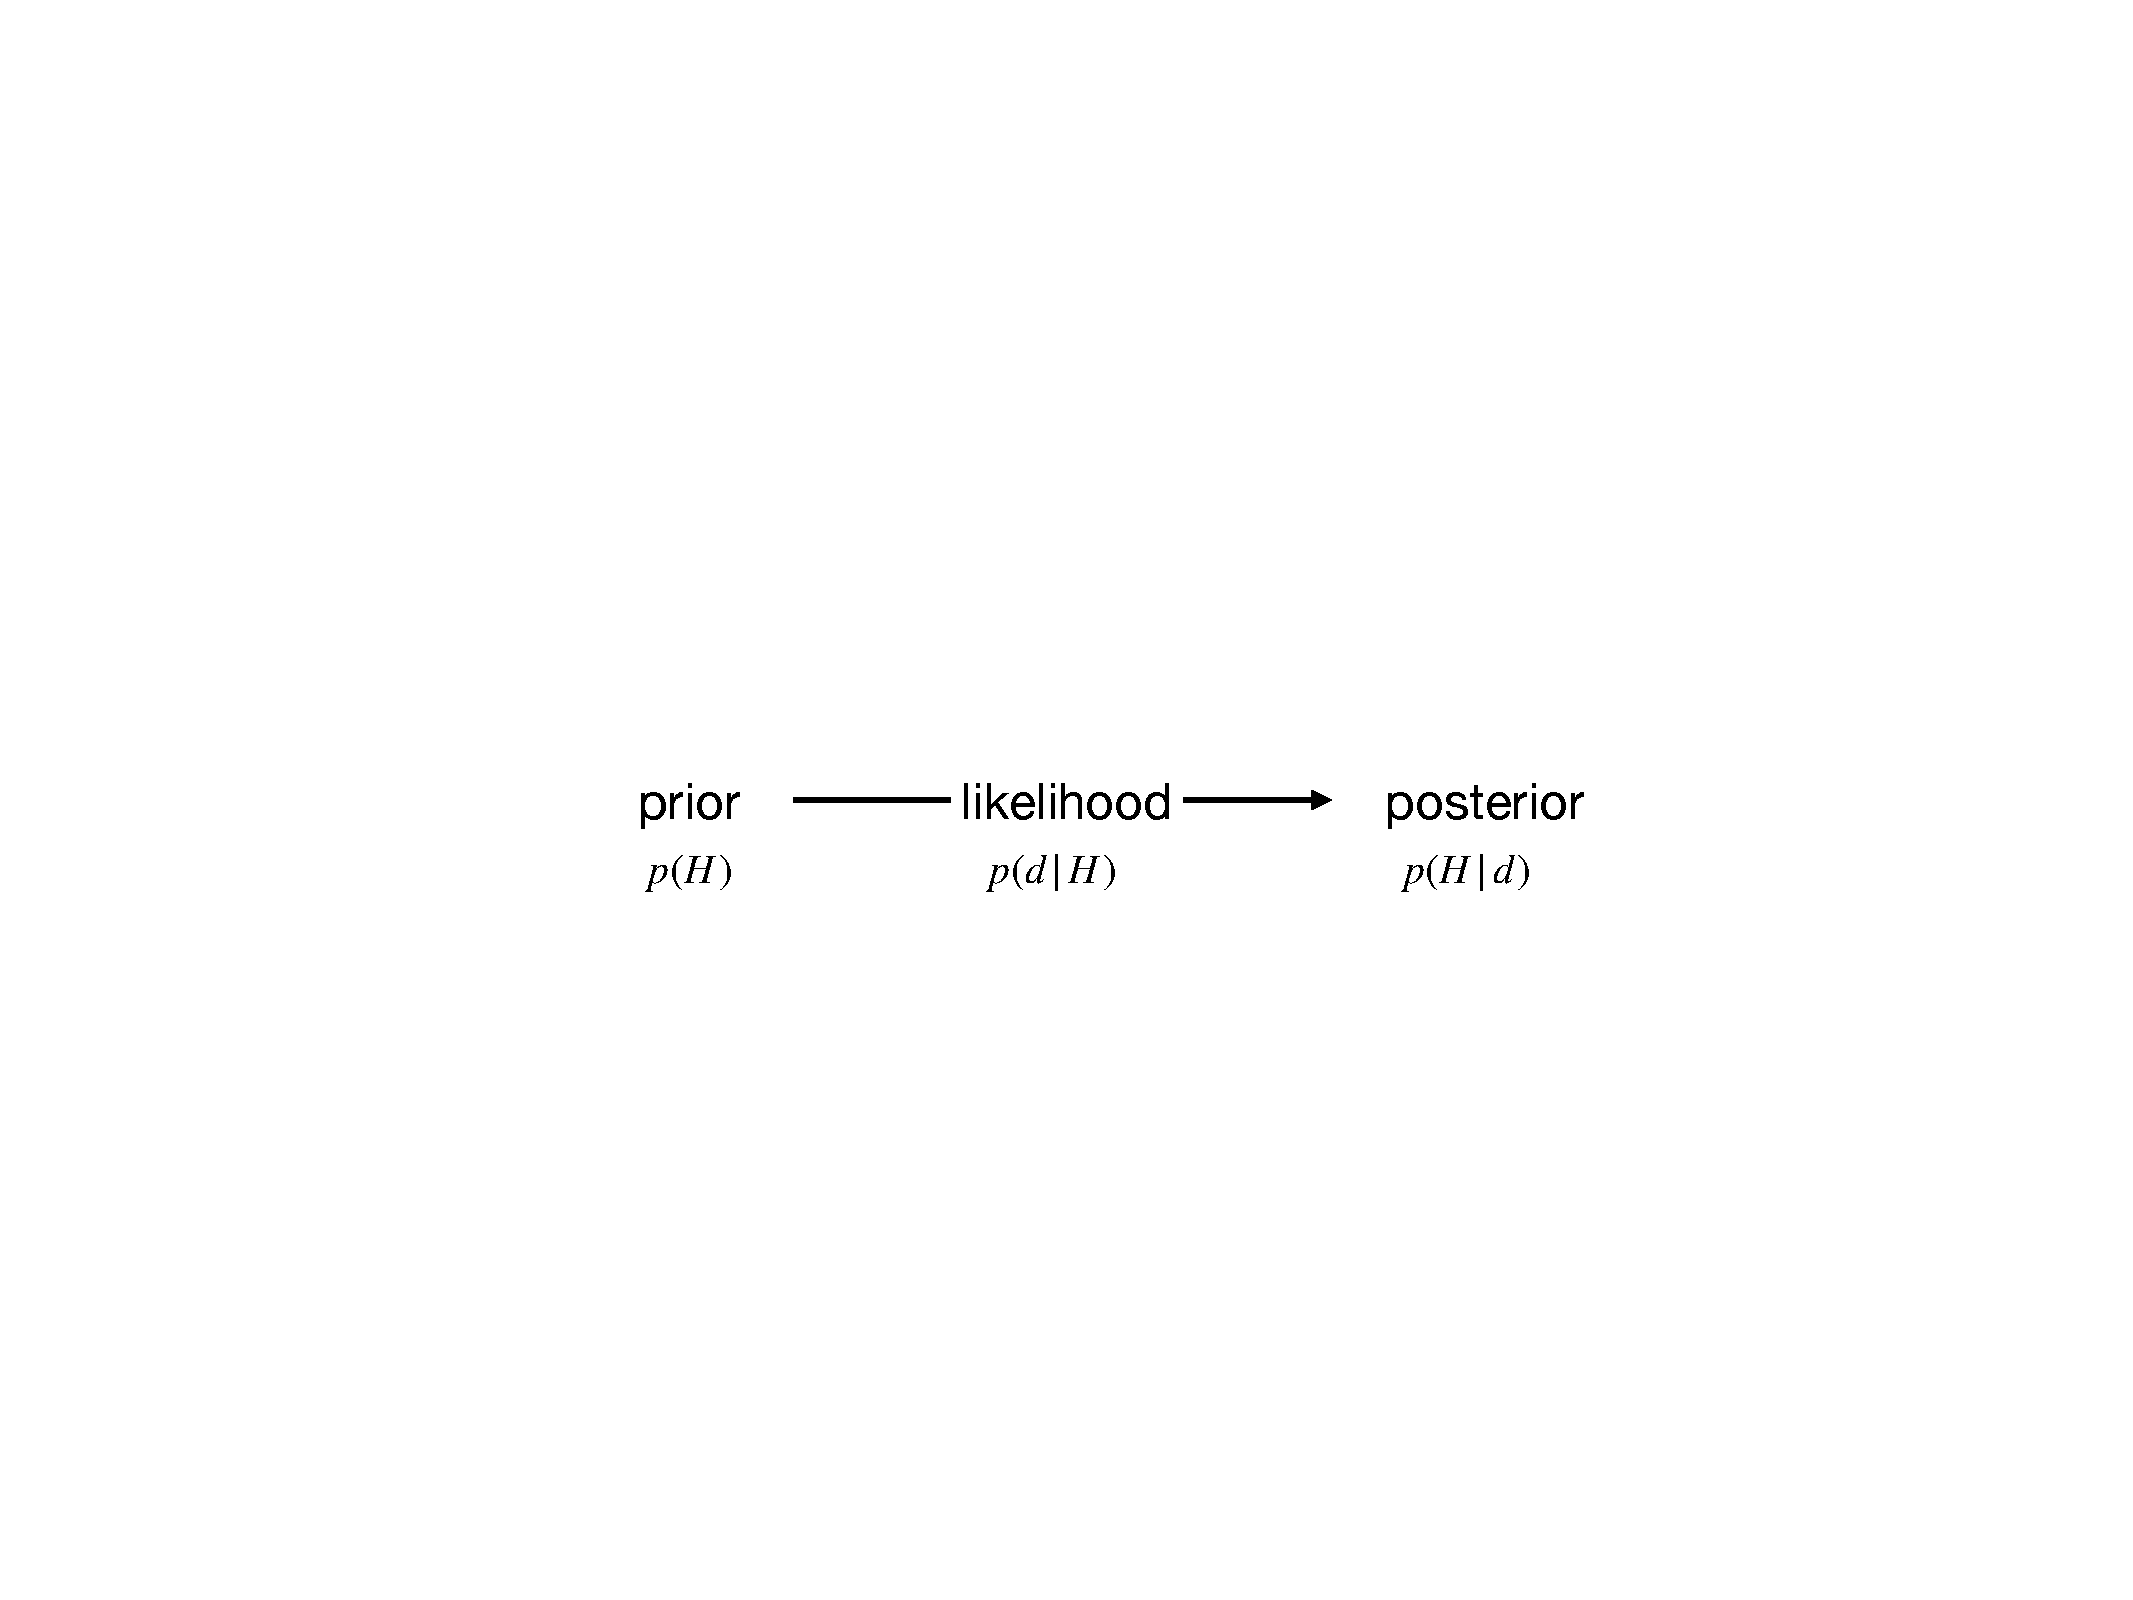
\includegraphics[width=0.45\textwidth]{Figures/bayes_theorem}
\caption{Schematic representation of Bayes' theorem.}
\label{f:bayes_theorem}
\end{center}
\end{figure}
%

In the context of searches for stochastic GW backgrounds,
Bayes' theorem has the form:
%
\be
p(S_{n_1}, S_{n_2}, S_h|d,{\cal M}_1) 
= \frac{p(d|S_{n_1}, S_{n_2}, S_h, {\cal M}_1)
p(S_{n_1}, S_{n_2}, S_h|{\cal M}_1)}{p(d|{\cal M}_1)}\,,
\ee
%
where $p(d|S_{n_1}, S_{n_2}, S_h,{\cal M}_1)$ is the likelihood
function \eqref{e:stochastic_likelihood}.
Here ${\cal M}_1$ is our signal+noise model and
$S_{n_1}$, $S_{n_2}$, $S_h$ are the parameters 
describing this model.
The quantity 
$p(S_{n_1}, S_{n_2}, S_h|d,{\cal M}_1)$ is the 
{\em joint} posterior probability distribution for
the parameters $S_{n_1}$, $S_{n_2}$, $S_h$ of 
model ${\cal M}_1$ given the data $d$.
The posterior distribution for $S_h$ alone is 
given by integrating over $S_{n_1}$, $S_{n_2}$:
%
\be
p(S_h|d,{\cal M}_1) 
= \int {\rm d}S_{n_1}\>\int{\rm d}S_{n_2}\>p(S_{n_1}, S_{n_2}, S_h|d,{\cal M}_1)\,.
\ee

%%%%%%%%%%%%%%%%%%%%%%%%%%%%%%%%%%%%%%%%%%%%%%%%%%%%
\subsubsection{Bayes factors and model selection}
\label{s:bayes_factors}

To assess which of two models 
${\cal M}_0$, ${\cal M}_1$ is more consistent with
the observed data $d$, we form 
the ratio of the posterior distributions 
$p({\cal M}_0|d)$, $p({\cal M}_1|d)$.
Using Bayes' theorem, we obtain
\be
\frac{p({\cal M}_1|d)}{p({\cal M}_0|d)} =
\frac{p(d|{\cal M}_1)\,p({\cal M}_1)}
{p(d|{\cal M}_0)\,p({\cal M}_0)}\,,
\ee
%
where the common evidence term $p(d)$ in
\eqref{e:bayes_theorem} has canceled out 
when taking the ratio of the two posteriors.
Thus, we see that the posterior odds ratio
$O_{12}(d)\equiv p({\cal M}_1|d)/p({\cal M}_0|d)$
is equal to the prior odds ratio
$O_{12}\equiv p({\cal M}_1)/p({\cal M}_0)$
times the {\em Bayes factor}
%
\be
{\cal B}_{10}(d)\equiv \frac{p(d|{\cal M}_1)}{p(d|{\cal M}_0)}\,.
\label{e:bayes_factor}
\ee
%
The numerator and denominator in the Bayes factor 
are the marginalized likelihoods obtained by 
marginalizing the full likelihood functions
$p(d|\theta_\alpha,{\cal M}_\alpha)$ over the 
model parameters $\theta_\alpha$:
%
\be
p(d|{\cal M}_\alpha) \equiv
\int {\rm d}\theta_\alpha\>
p(d|\theta_\alpha, {\cal M}_\alpha)p(\theta_\alpha|{\cal M}_\alpha)\,,
\ee
%
where $\alpha=0,1$ labels the two models.
If there is no reason to a~priori prefer one model over 
the other (i.e., if the prior odds ratio $O_{10}=1$), then the 
posterior odds ratio for the two models is equal to the 
Bayes' factor, $O_{10}(d) = {\cal B}_{10}(d)$.

Using the above definitions, we are now in a position to 
relate Bayesian and frequentist inference, at least in the 
case where the data are informative.
By this we mean that the likelihood function for a given
model is peaked relative to the prior probability 
distribution for its model parameters 
(Figure~\ref{f:informative_data}).
For this case, the marginalized likelihoods functions 
have the approximate form 
%
\be
p(d|{\cal M}_\alpha) 
%\equiv\int {\rm d}\theta_\alpha\>
%p(d|\theta_\alpha, {\cal M}_\alpha)p(\theta_\alpha,{\cal M}_\alpha)
\simeq
p(d|\hat\theta_\alpha, {\cal M}_\alpha)
\,{\Delta V_\alpha}/{V_\alpha}\,,
\ee
%
where $\hat\theta_\alpha$ denote the parameter values that
maximize the likelihood, $\Delta V_\alpha$ is the range of
parameter values over which the likelihood is peaked, and 
$V_\alpha$ denotes the full parameter volume.
This approximation is called the {\em Laplace approximation}.
%
\begin{figure}[htbp!]
\begin{center}
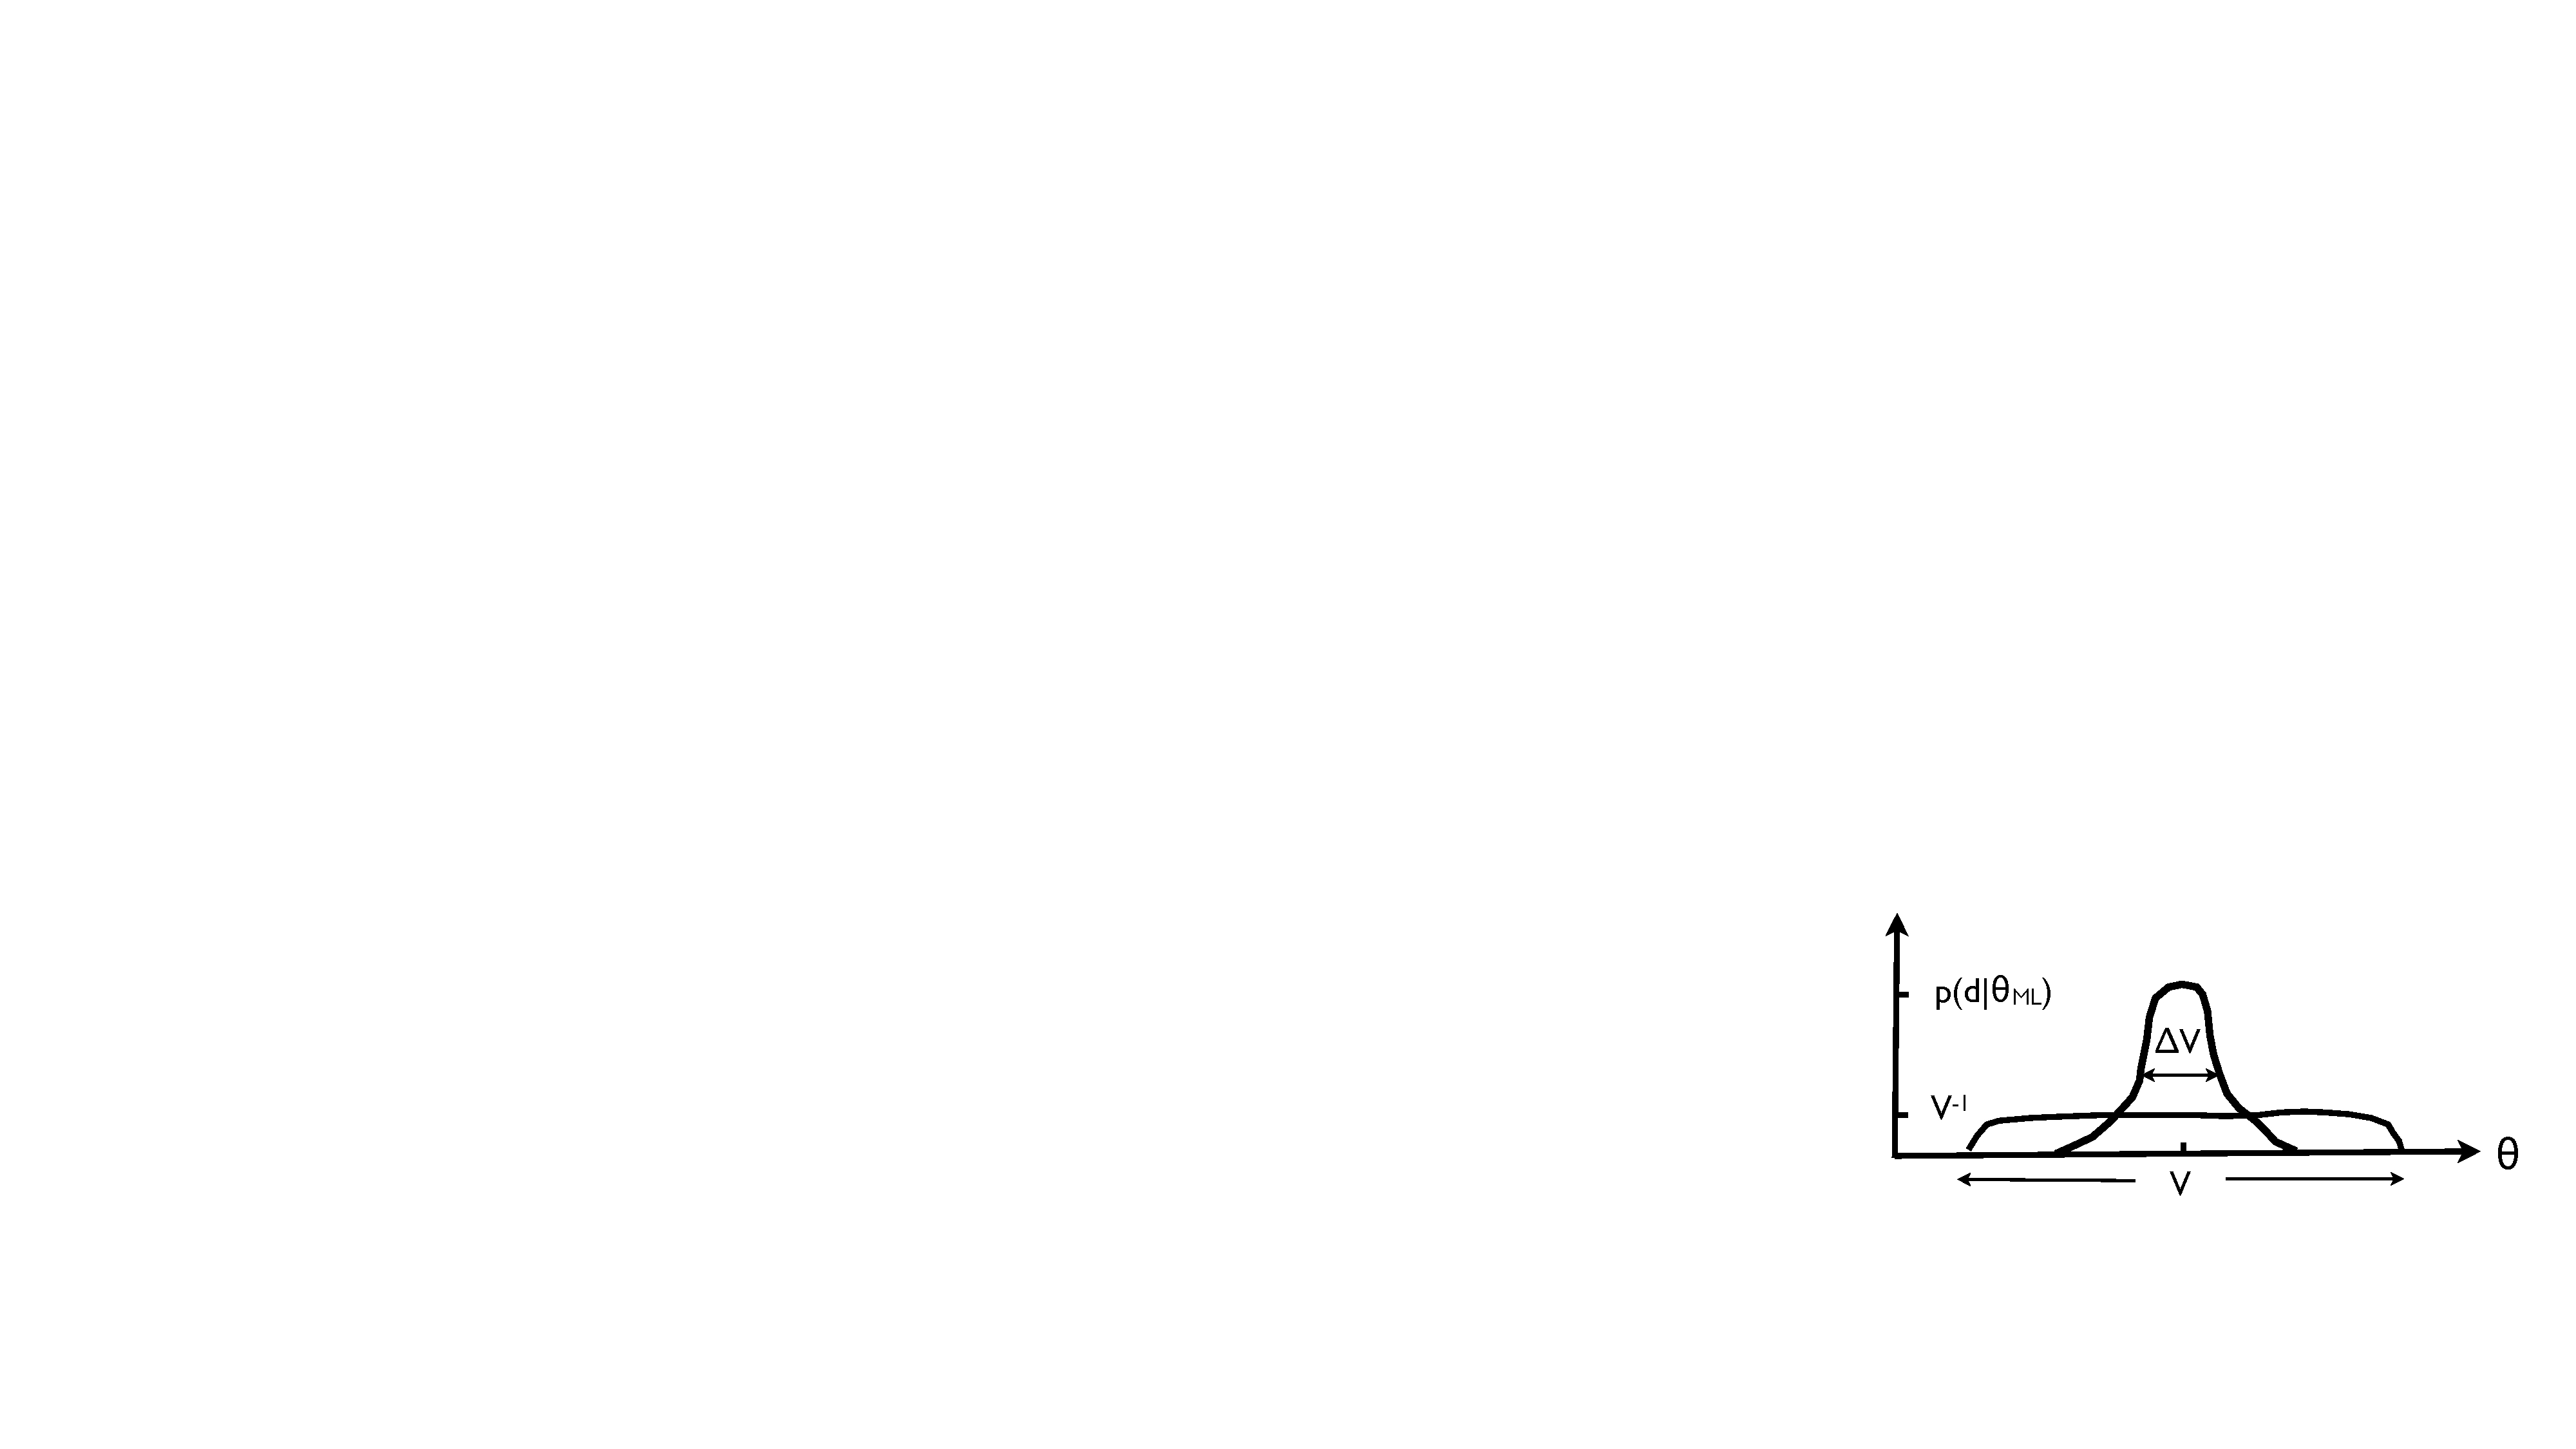
\includegraphics[width=0.5\textwidth]{Figures/informative_data}
\caption{Schematic representation of the likelihood function 
$p(d|\theta,{\cal M})$ and prior probability distribution 
$p(\theta|{\cal M})$ for the model parameters $\theta$,
when the data $d$ are informative.
In this case, the likelihood function is peaked relative to the 
prior probability distribution, with maximum at 
$\theta=\hat\theta$ and characteristic width $\Delta V$.
The full parameter space volume is denoted by $V$.}
\label{f:informative_data}
\end{center}
\end{figure}
%
Substituting these expressions into \eqref{e:bayes_factor} we find
%
\be
{\cal B}_{10}(d) 
\equiv\frac{p(d|{\cal M}_1)}{p(d|{\cal M}_0)}
\simeq \frac{p(d|\hat\theta_1,{\cal M}_1)}{p(d|\hat\theta_0,{\cal M}_0)}
\,\frac{\Delta V_1/V_1}{\Delta V_0/V_0}
\simeq\Lambda_{\rm ML}(d)
\,\frac{\Delta V_1/V_1}{\Delta V_0/V_0}\,,
\ee
where $\Lambda_{\rm ML}(d)$ is just the maximum-likelihood
ratio for the two models.
This last expression can also be written as
%
\be
2\ln({\cal B}_{10}(d)) \simeq \Lambda(d) + 
2\ln\left(\frac{\Delta V_1/V_1}{\Delta V_0/V_0}\right)
\ee
%
where $\Lambda(d)\equiv 2\ln(\Lambda_{\rm ML}(d))$
plays the role of a frequentist detection statistic, 
and the last term is an Occam's factor that penalizes
models that use more parameter space volume than needed
to fit the data.
As shown in~\eqref{e:Lambda}, $\Lambda(d)$ is effectively
a squared signal-to-noise ratio.
The key observation here is that the ratio of marginalized
likelihoods is well approximated by a maximum-likelihood 
ratio times an Occam's penalty factor when the data are informative.

%%%%%%%%%%%%%%%%%%%%%%%%%%%%%%%%%%%%%%%%%%%%%%%%%%
\subsubsection{Bayesian signal priors}
\label{s:signal_priors}

The final piece of information that we will need when 
discussing the Bayesian search for BBH mergers in 
Section~\ref{s:nonstationary} is related to the choice 
of signal prior.
We shall see in that section that by choosing the 
signal prior appropriately, we can properly model 
the popcorn-like nature of the GWB produced by BBH 
mergers.

Here, we illustrate the effect of chosing different
priors for two simple cases: 
(i) a deterministic GW signal (a sinusoid), and 
(ii) a Gaussian-stationary stochastic background in 
Gaussian-distributed noise.
For both of these cases, the difference between the 
observed data $d$ and signal model $h$ is just 
the noise $n$.
So we can write down a generic likelihood function for 
the data $d$ by equating it to the 
Gaussian-distributed likelihood for the residuals $d-h$:
%
\begin{equation}
p(d|C_n,h) \equiv p_n(d-h|C_n) 
= \frac{1}{\sqrt{{\rm det}(2\pi C_n)}}\,
\exp\left[-\frac{1}{2}(d-h)^T C_n^{-1}(d-h)\right]\,,
\label{e:likelihood_generic}
\ee
%
where $C_n$ is the noise covariance matrix.
To proceed further we need to specify the form of the 
signal $h$ in more detail.

(i) For a deterministic GW signal, we expect the signal
samples to have a precise form, e.g., a sine wave
parametrized by its amplitude, frequency, and initial phase 
(Figure~\ref{f:det_signal_prior}).
For this case we would have the prior probability distribution
%
\begin{equation}
p(h|A, f_0, \phi_0)
=\delta\left(h(t)- A\sin(2\pi f_0 t + \phi_0)\right)\,.
\label{e:prior_deterministic}
\ee
%
Multiplying the likelihood \eqref{e:likelihood_generic}
by this prior and marginalizing over the signal samples
$h$ yields
%
\be
\begin{aligned}
&p(d|C_n,A,f_0,\phi_0)
\\
&\quad
\equiv \int {\rm d}h\>p_n(d-h|C_n)p(h|A, f_0, \phi_0) 
\\
&\quad
=\frac{1}{\sqrt{{\rm det}(2\pi C_n)}}\,
\exp\left[-\frac{1}{2}\sum_{i,j}
(d_i-A\sin(2\pi f_0 t_i + \phi_0)) 
[C_n^{-1}]_{ij}(d_j-A\sin(2\pi f_0 t_j + \phi_0))\right]\,.
\label{e:likelihood_deterministic}
\end{aligned}
\ee
%
This marginalized likelihood with priors on the range of
parameter values for $A$, $f_0$, $\phi_0$ and covariance
matrix $C_n$ for the noise then completely define the deterministic 
signal+noise model.
%
\begin{figure}[htbp!]
\begin{center}
\subfigure[]{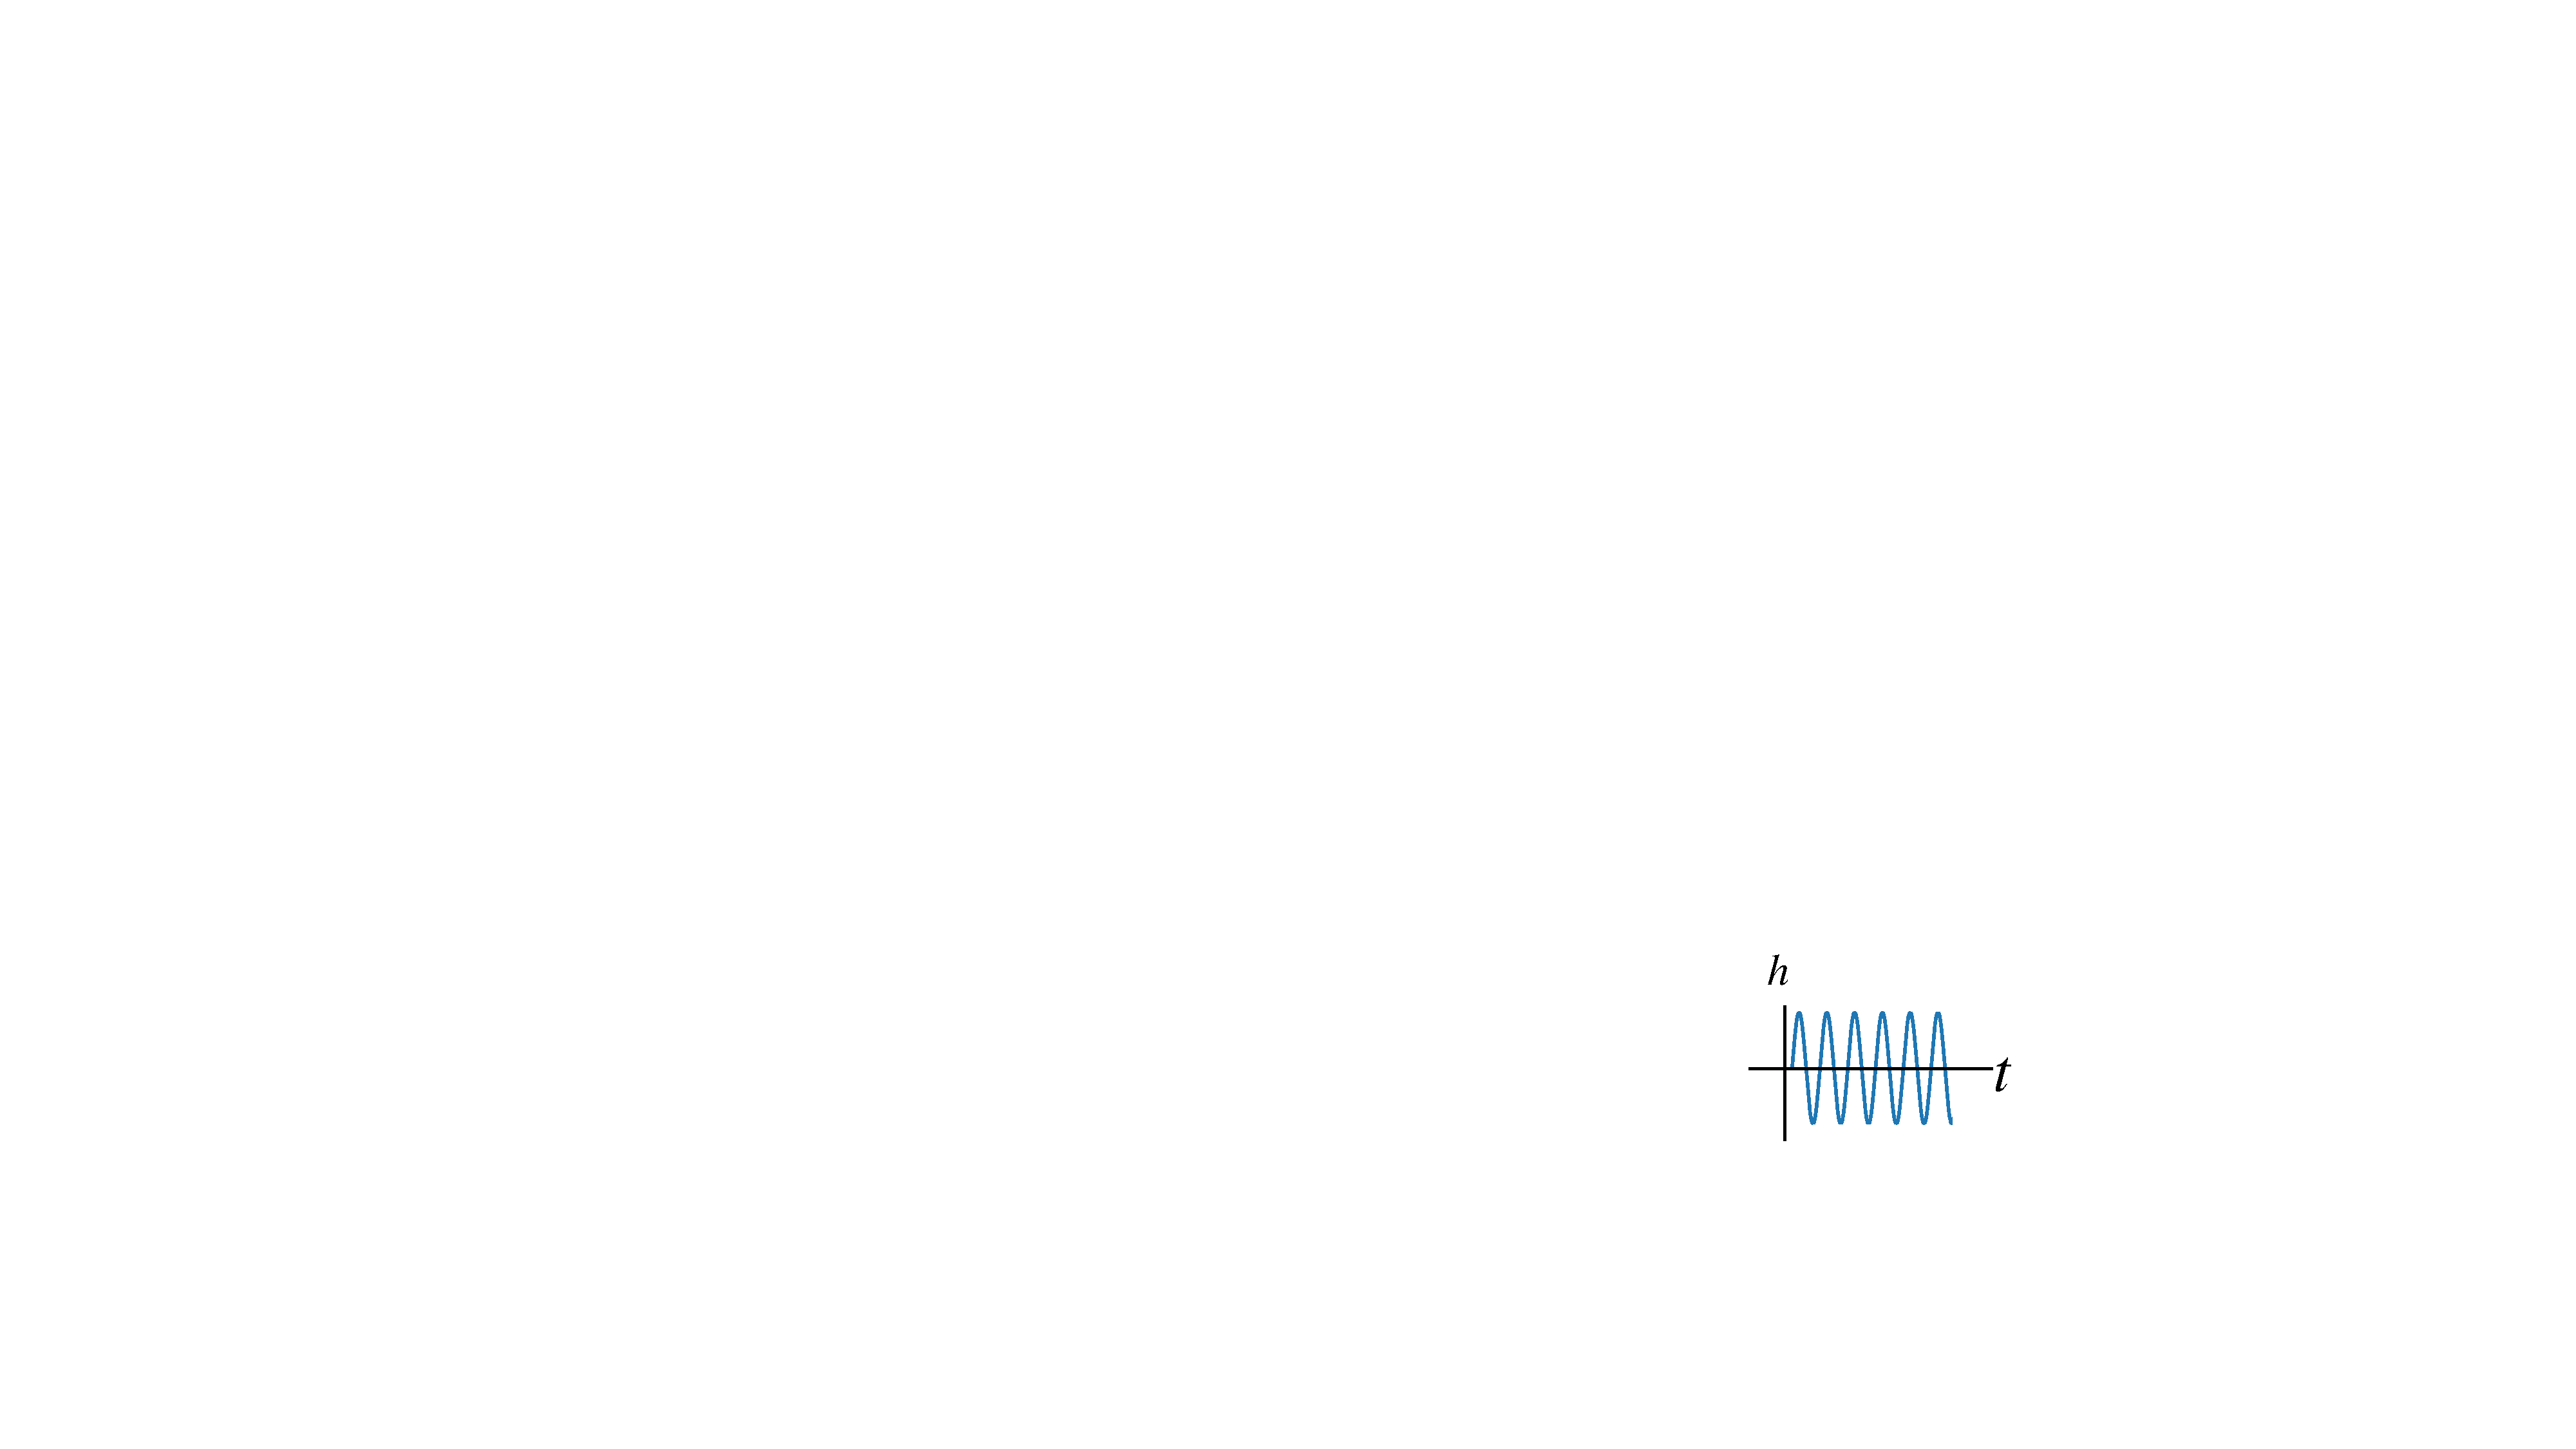
\includegraphics[width=0.25\textwidth]{Figures/sinusoid_prior}
\label{f:det_signal_prior}}
\hspace{1 in}
\subfigure[]{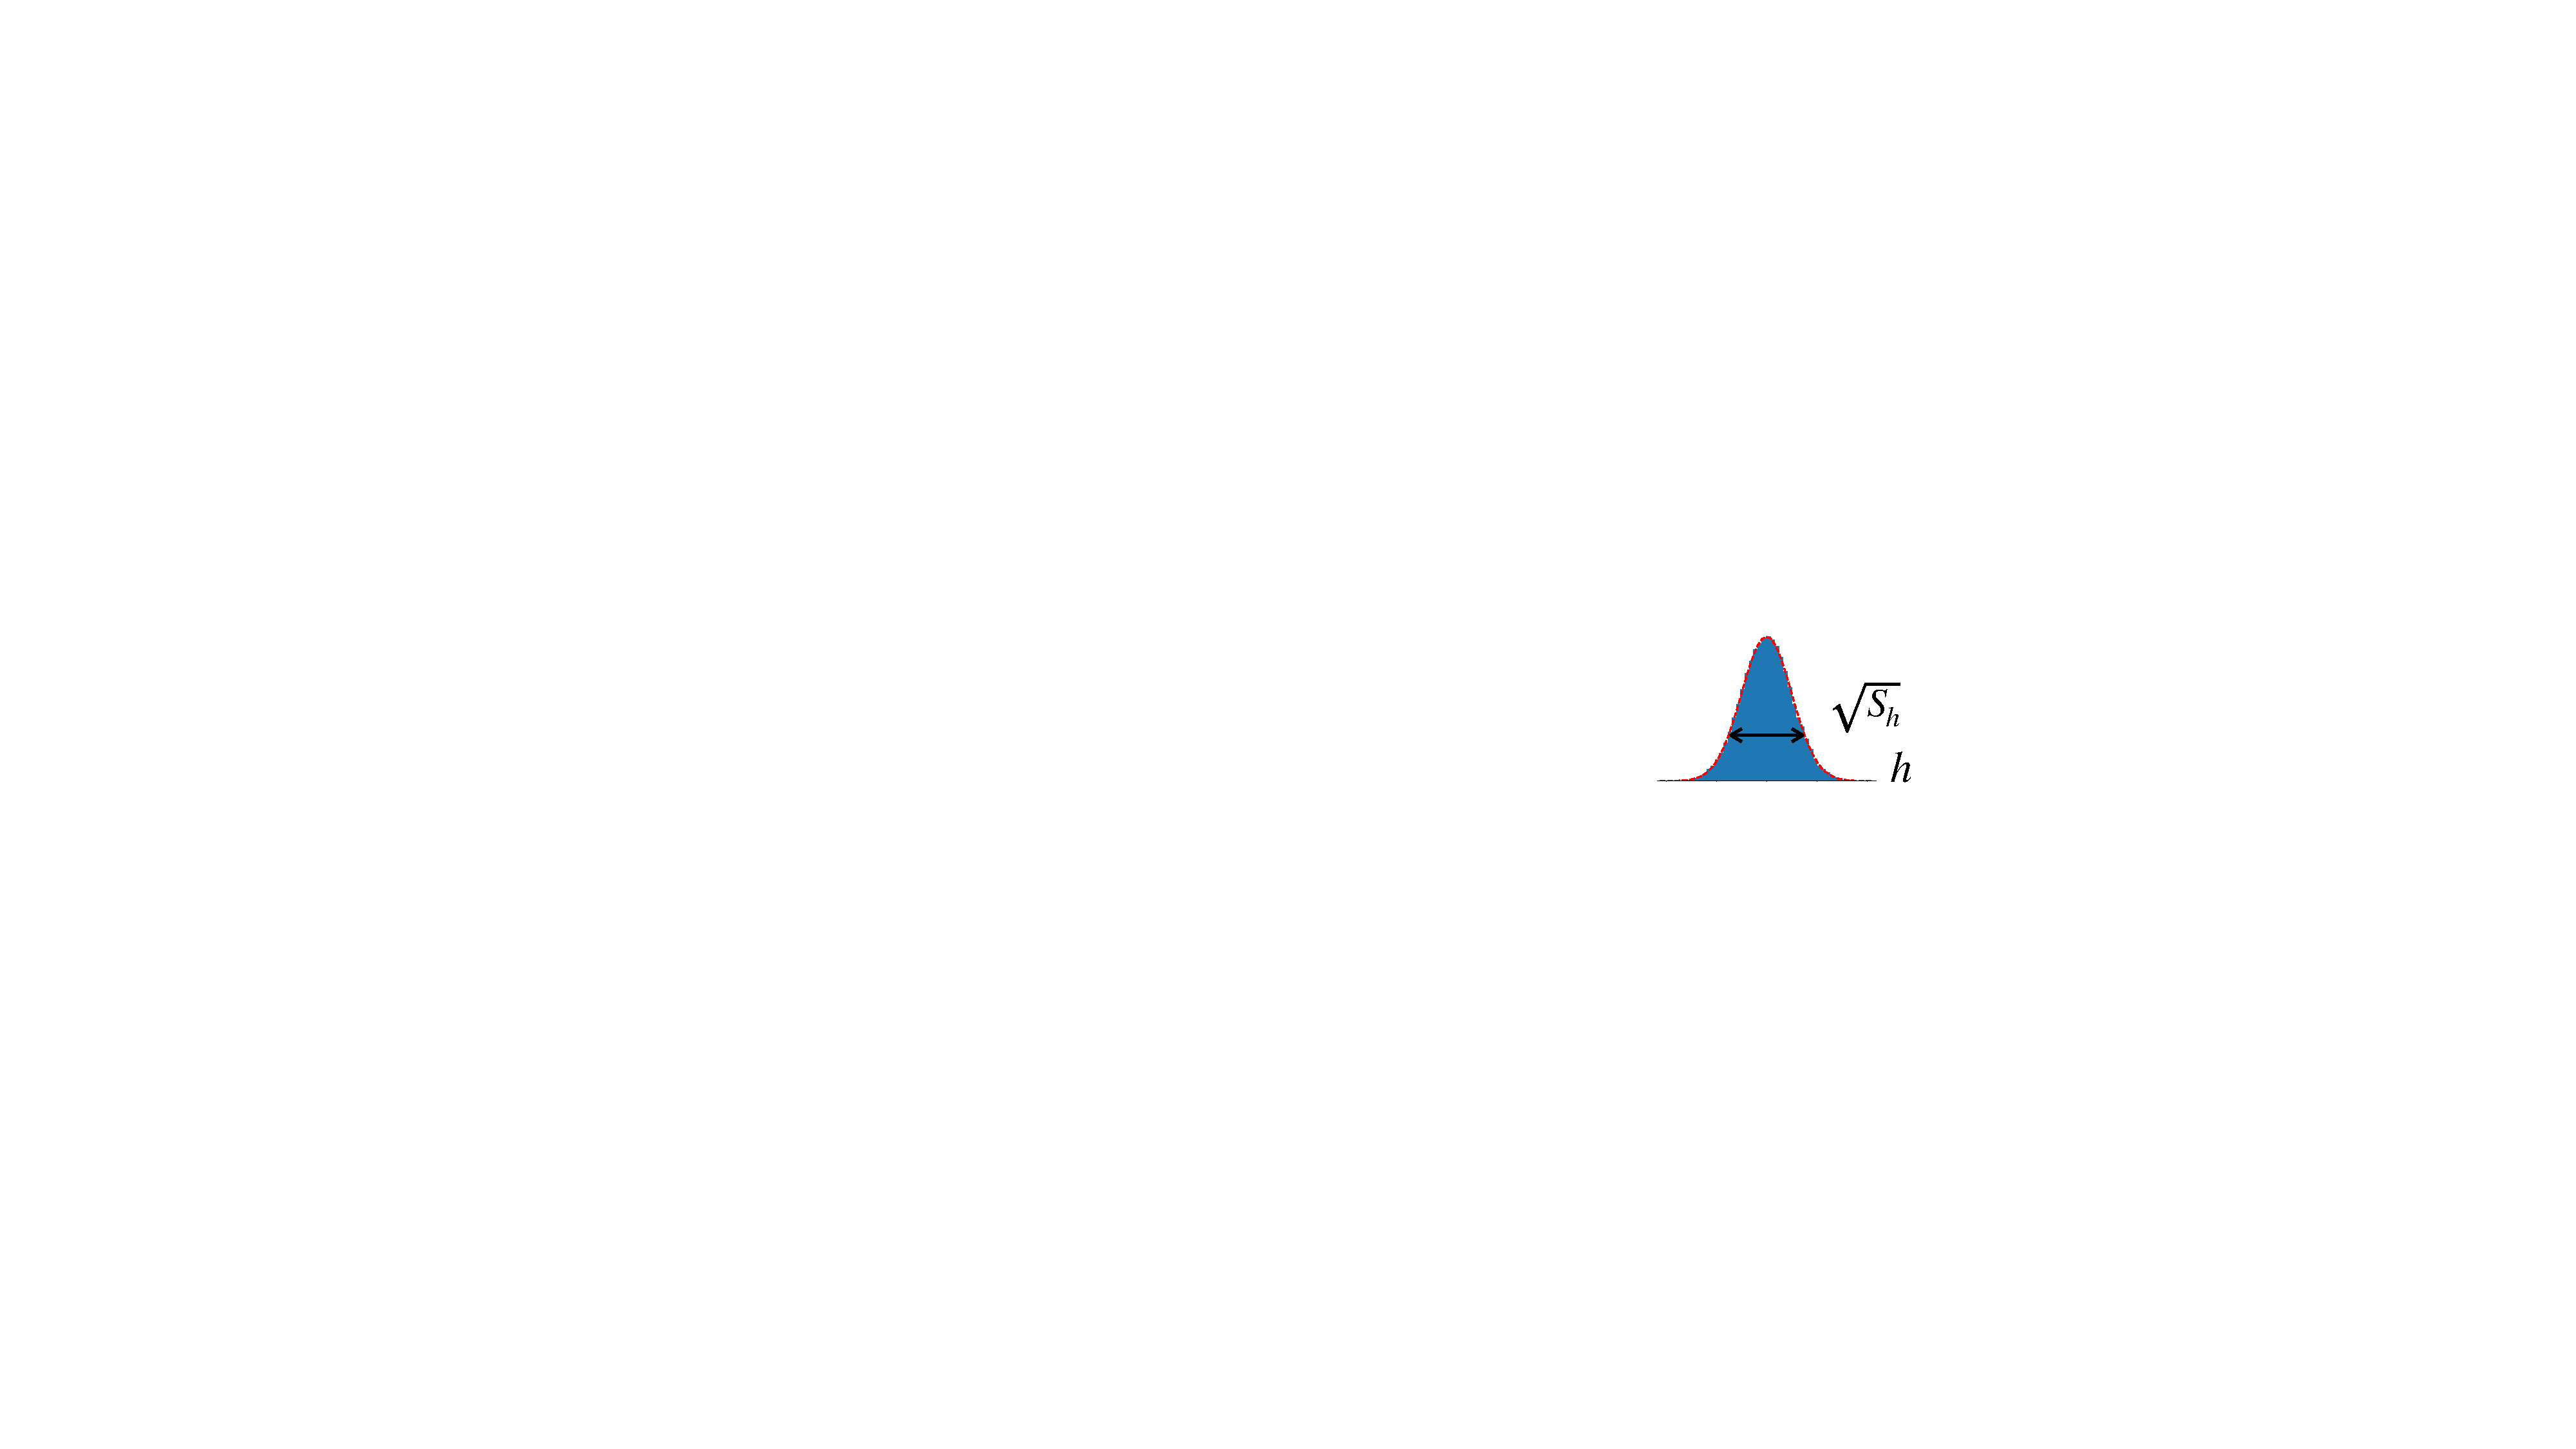
\includegraphics[width=0.25\textwidth]{Figures/stochastic_prior}
\label{f:stoch_signal_prior}}
\caption{Different signal priors for $h(t)$.
Panel (a): Determinsitic (sinusoid) signal prior.
Panel (b): Stochastic signal prior.
For the stochastic signal prior, $h(t)$ values are drawn from a
Gaussian distribution with variance $S_h$.}
\label{f:det_stoch_signal_priors}
\end{center}
\end{figure}
%

(ii) For a stohastic GW signal, we don't know what the
individual samples $h$ will be, other than that they are
drawn from some probability distribution.  
Taking that distribution to be a Gaussian with zero mean
and variance $S_h$ (Figure~\ref{f:stoch_signal_prior}),
we have
%
\begin{equation}
p(h|S_h) 
= \frac{1}{\sqrt{2\pi S_h}}\,\exp\left[-\frac{1}{2}\frac{h^2}{S_h}\right]\,.
\label{e:stoch-prior}
\ee
%
Multiplying the likelihood \eqref{e:likelihood_generic}
by this prior and marginalizing over the signal samples
$h$ for this case yields
%
\begin{equation}
p(d|C_n,S_h) 
\equiv\int {\rm d}h\>p_n(d-h|C_n)p(h|S_h) 
= \frac{1}{\sqrt{{\rm det}(2\pi C)}}\,\exp\left[-\frac{1}{2}d^T C^{-1} d\right]
\ee
%
where $C \equiv C_n + S_h$.
This marginalized likelihood with a prior on the 
variance $S_h$ for the stochastic signal samples 
and covariance matrix $C_n$ for the noise then
completely defines the Gaussian-stationary stochastic
signal+noise model.

In Exercise~\ref{exer:10} you are asked to extend the
above analysis for a stochastic background to the 
case of two detectors with uncorrelated detector noise.
Starting with the generic two-detector likelihood
%
\begin{equation}
p(d|C_n,h) \equiv p_n(d-h|C_n) 
= \frac{1}{\sqrt{{\rm det}(2\pi C_n)}}\,\exp\left[-\frac{1}{2}(d-h)^T C_n^{-1}(d-h)\right]
\ee
%
where
%
\begin{equation}
C_n = \begin{bmatrix}
S_{n_1} & 0\\
0 & S_{n_2}
\end{bmatrix}\,.
\ee
%
and marginalizing over $h$ using \eqref{e:stoch-prior}, 
you should find
%
\be
p(d|C_n, S_h)
= \frac{1}{\sqrt{{\rm det}(2\pi C)}}\,\exp\left[-\frac{1}{2}d^T C^{-1} d\right]
\ee
%
where
%
\begin{equation}
C = \begin{bmatrix}
S_{n_1} + S_h & S_h\\
S_h & S_{n_2} + S_h
\end{bmatrix}\,.
\ee
%
This marginalized likelihood is usually taken as the starting
point for all stochastic cross-correlation searches using
multiple detectors; see~\eqref{e:stochastic_likelihood}.

%%%%%%%%%%%%%%%%%%%%%%%%%%%%%%%%%%%%%%%%%%%%%%%%%%%%%%%
\section{Searching for the background of binary black-hole mergers}
\label{s:nonstationary}

As discussed in Section~\ref{s:BBH-BNS-LIGO}, the non-continuous 
popcorn-like background from BBH mergers is a potential signal 
for advanced LIGO and Virgo.
The recent detections of several large signal-to-noise ratio
BBH and BNS mergers imply the existence of a stochastic GW 
background of the more distant, weaker events.
In 2018, Smith \& Thrane~\cite{Smith-Thrane:2018} 
proposed an alternative to the standard cross-correlation 
method (Section~\ref{s:correlations})
to search for the BBH component, optimally suited for the 
intermitent nature of the signal.
This was done by describing the BBH 
background with a ``mixture" signal prior consisting of
a BBH chirp in a certain fraction $\xi$ of the analyzed 
segments, and noise only for the remaining segments.
Also, as the individual signals will not be resolvable, they 
choose to marginalize over the BBH chirp parameters 
leaving only the probabity parameter $\xi$ (which is 
simply related to the rate of BBH signals) to estimate.
Although in principle they can do the analysis with a
single detector, they use two detectors to help 
discriminate against glitches.

\subsection{Analysis details}

The key components of their analysis are as follows:
\smallskip

\noindent
1) Begin by splitting data in short (e.g., 4 sec) segments, 
which should contain at most one BBH merger.

\smallskip
\noindent
2) Choose a mixture signal prior for the signal model:
%
\begin{equation}
p(h|\xi, \vec\lambda) 
= \xi\,\delta\left(h-{\rm chirp}(\vec\lambda)\right) +
(1-\xi)\,\delta(h)\,,
\label{e:mixture-signal-prior}
\ee
%
which consists of a BBH chirp signal with probabiity
$\xi$ and noise only ($h=0$) with probability $(1-\xi)$
(Figure~\ref{f:mixture_signal_priors}).
This mixture signal prior captures the non-continuous
popcorn-like nature of the BBH mergers.
%
\begin{figure}[htbp!]
\begin{center}
\subfigure[]{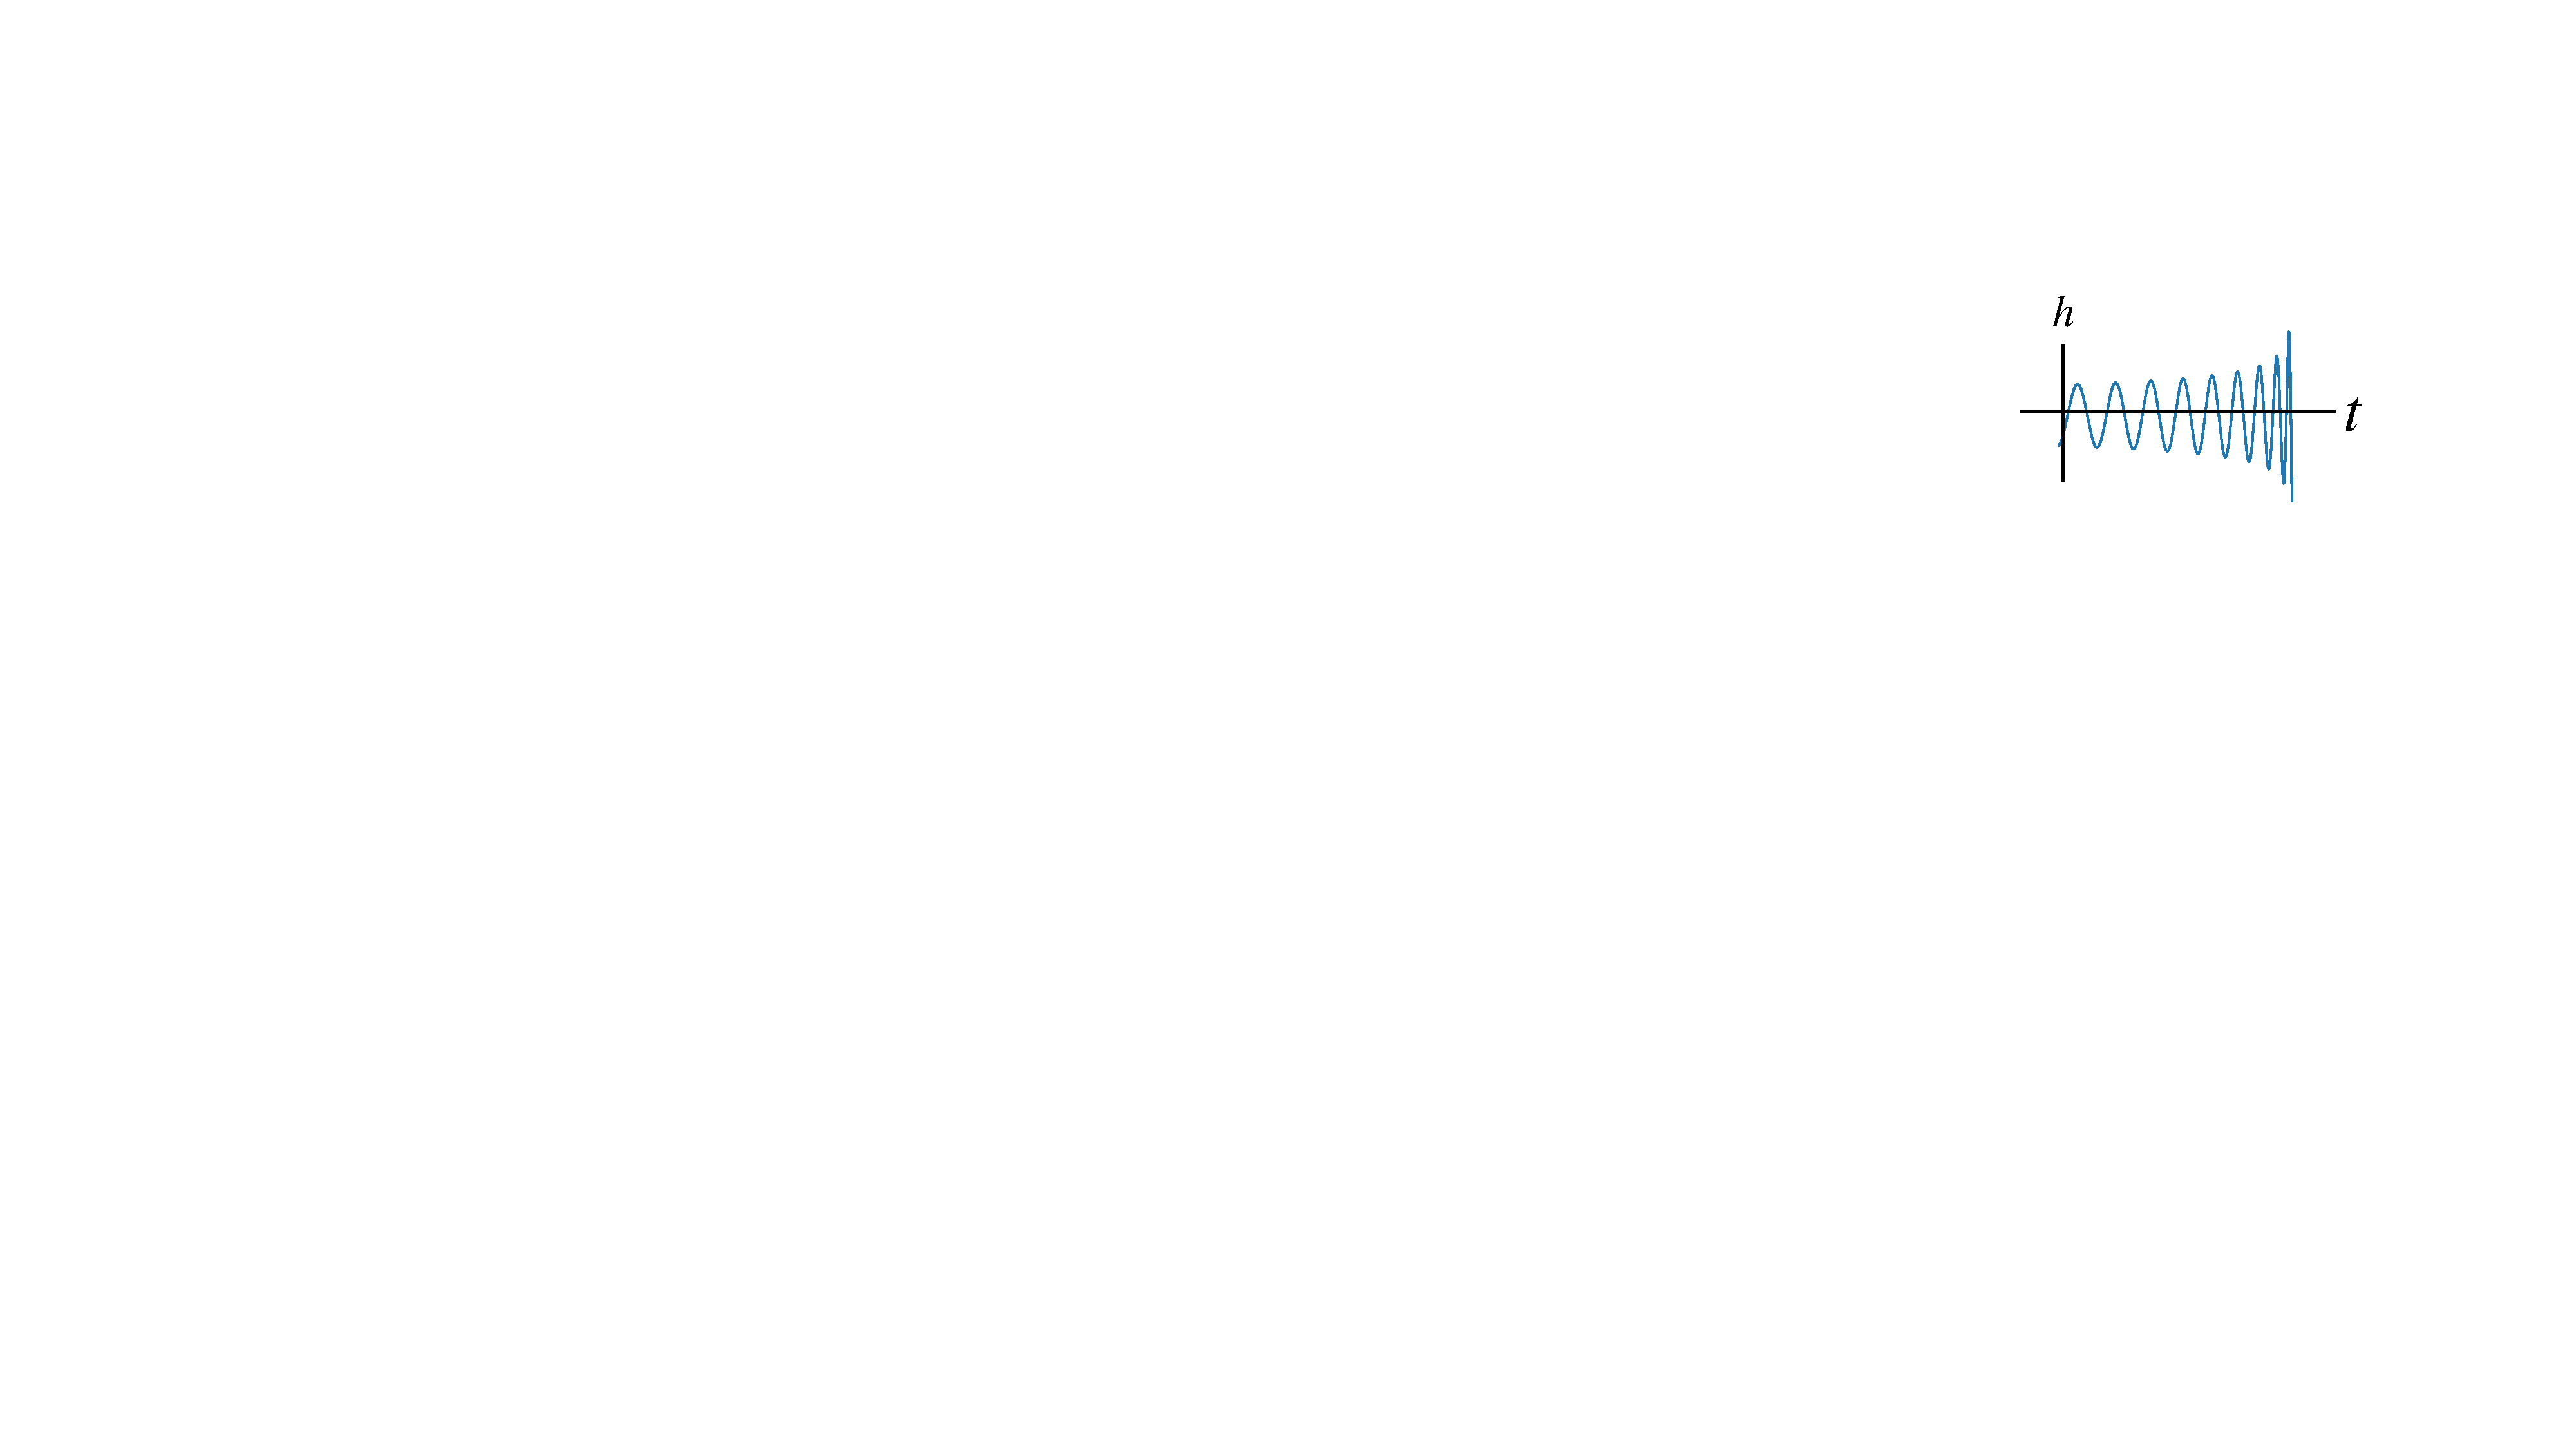
\includegraphics[width=0.25\textwidth]{Figures/chirp_prior}}
\hspace{1 in}
\subfigure[]{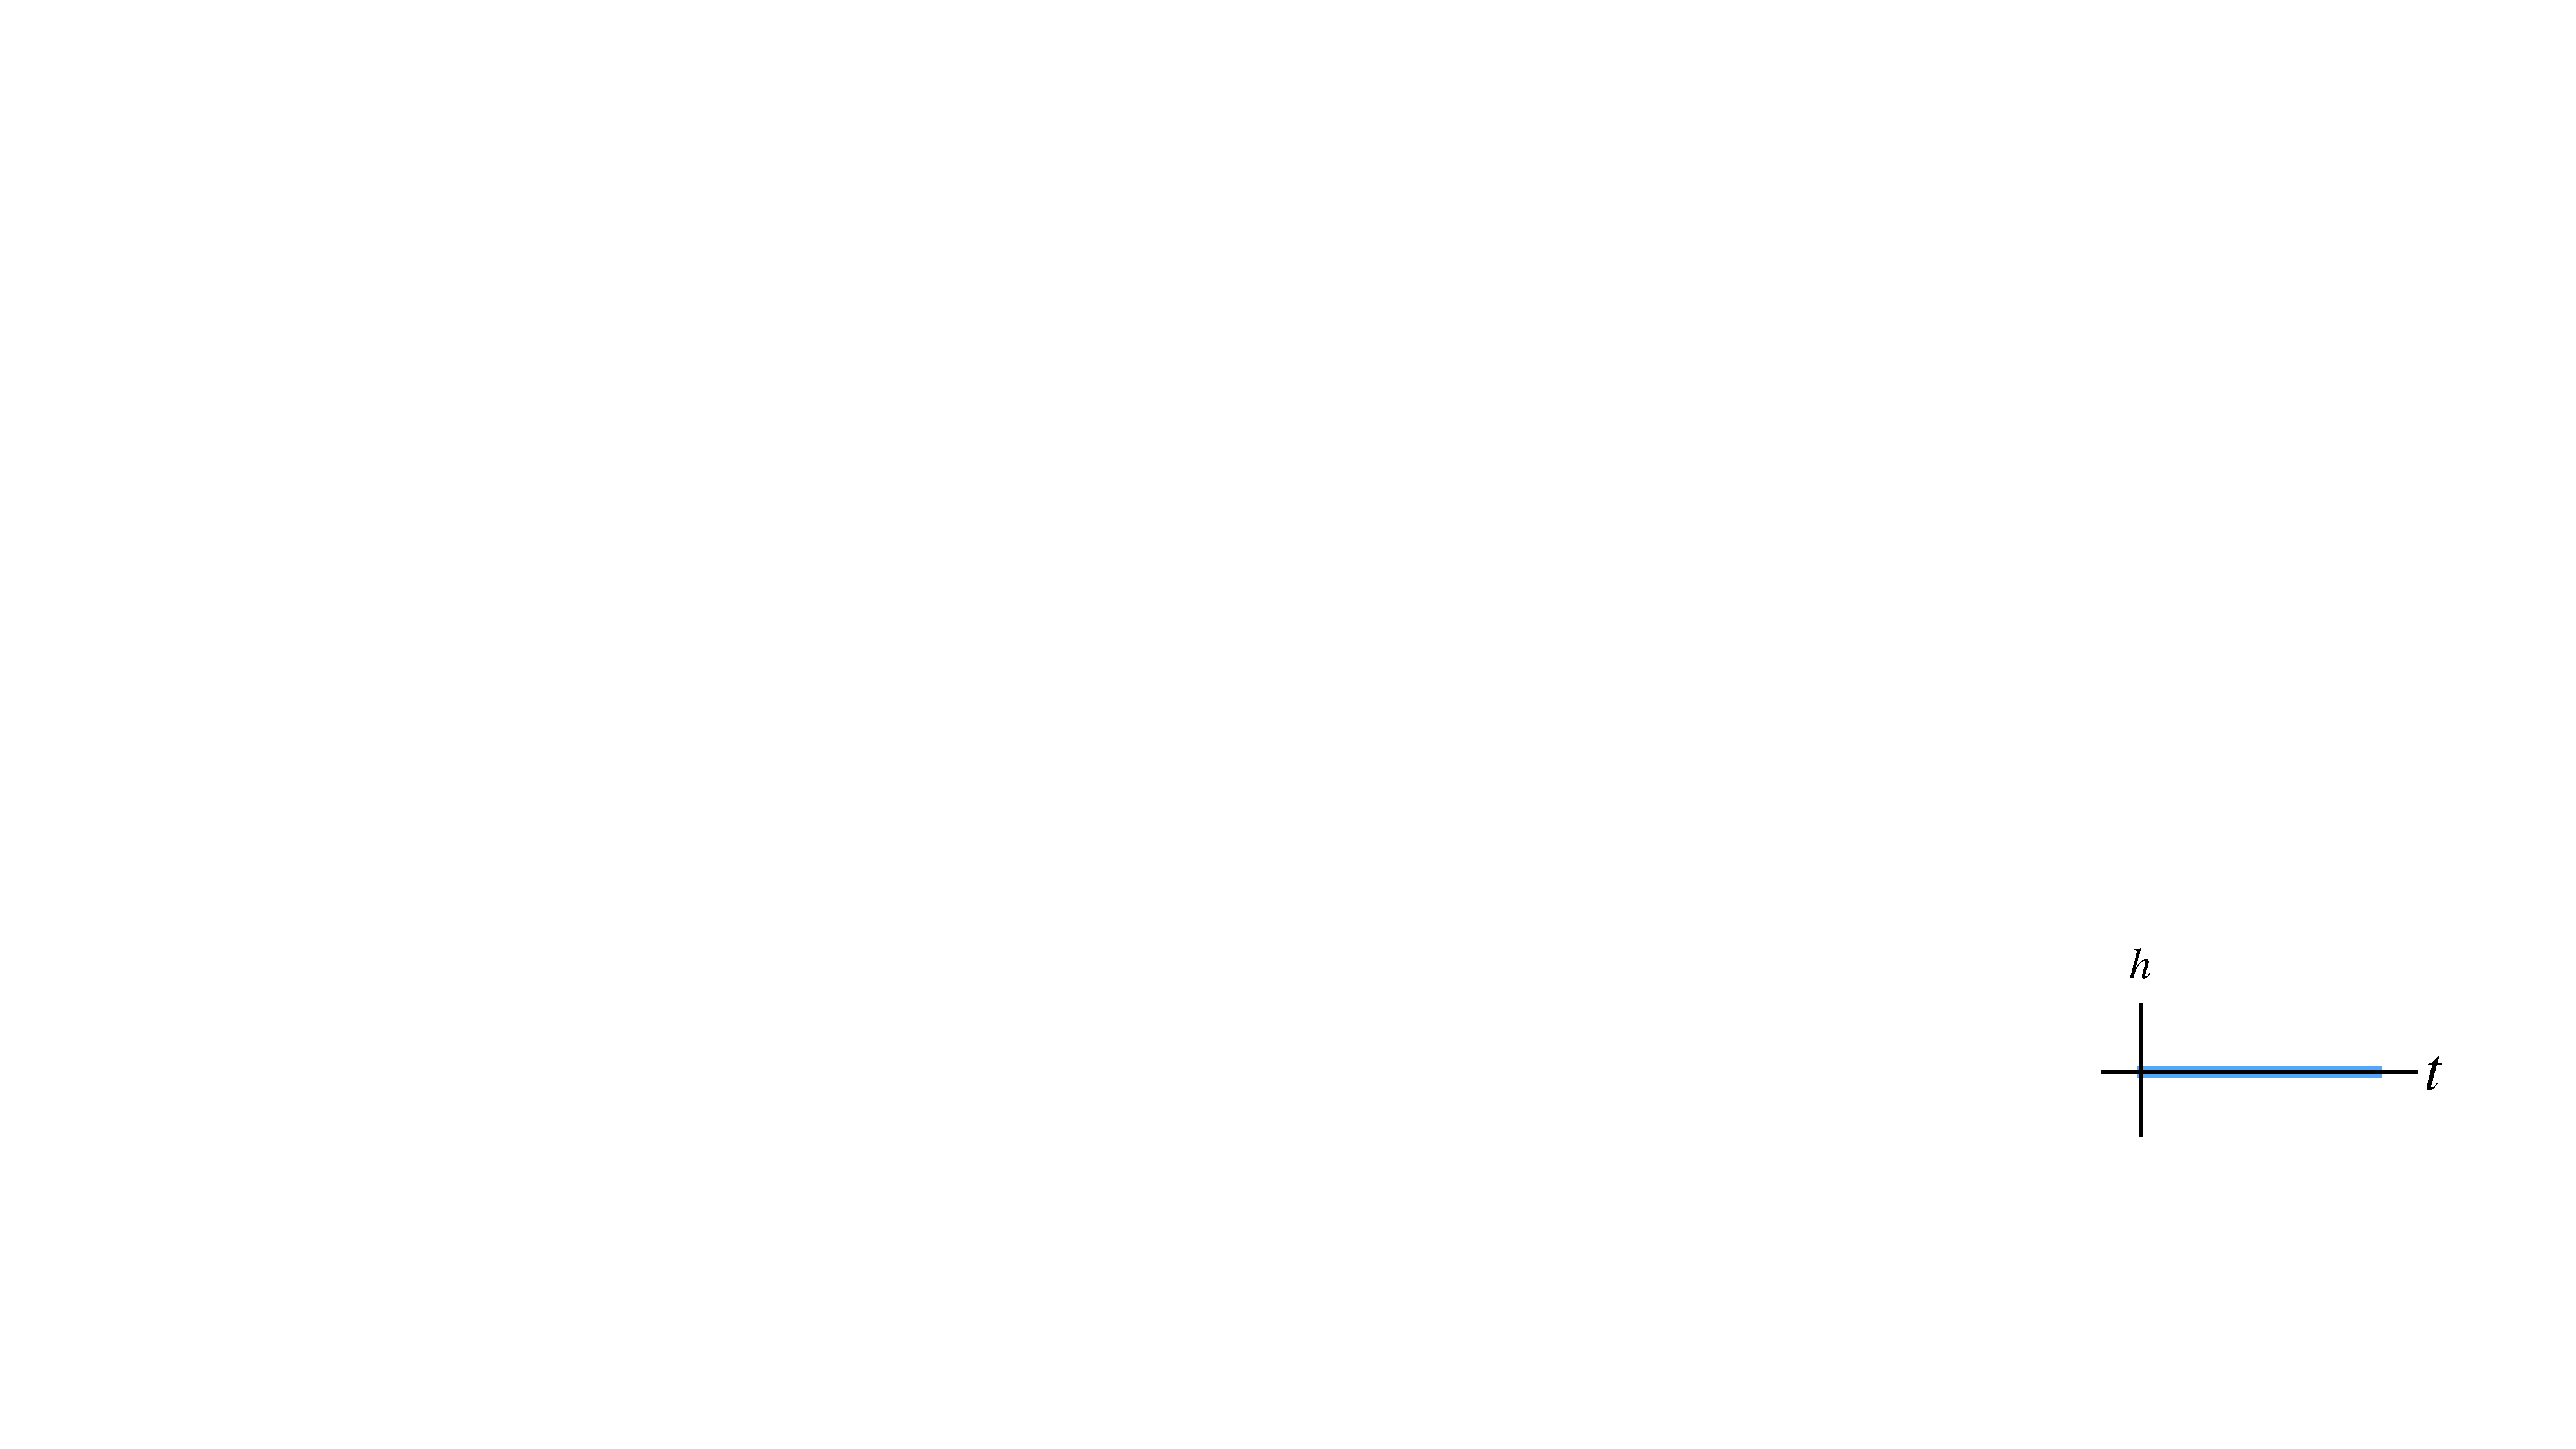
\includegraphics[width=0.25\textwidth]{Figures/no_signal_prior}}
\caption{The two components of the mixture signal prior for the 
Bayesian BBH merger search.
Panel (a): With probability $\xi$, the signal prior for $h(t)$ is a 
chirp waveform.
Panel (b): With probability $(1-\xi)$, the signal prior for $h(t)$ is
noise only, i.e., $h(t)=0$.}
\label{f:mixture_signal_priors}
\end{center}
\end{figure}

\smallskip
\noindent
3) For each segment of data $d_i$, marginalize
the standard likelihood function
%
\begin{equation}
p(d_i|C_n,h)\equiv p_n(d_i-h|C_n)
\ee
%
over the signal prior \eqref{e:mixture-signal-prior}:
%
\be
\begin{aligned}
p(d_i|\xi, \vec\lambda, C_n)
&=\int {\rm d}h\>p(d_i|C_n,h)p(h|\xi,\vec\lambda)
\\
&= \xi\,p_n(d_i-{\rm chirp}(\vec\lambda)|C_n) + (1-\xi)\,p_n(d_i|C_n)\,.
\end{aligned}
\ee
%
Note that this is a mixture Gaussian likelihood function.

\smallskip
\noindent
4) Further marginalize over the BBH signal
parameters $\vec\lambda$, and use an estimate of 
the detector noise thus fixing $C_n\equiv \bar C_n$:%
%
\begin{equation}
p(d_i|\xi)=\int {\rm d}\vec\lambda\>
p(d_i|\xi,\vec\lambda, \bar C_n)\,p(\vec\lambda)
\equiv (S_i-N_i)\xi + N_i\,.
\label{e:p(d_i|xi)}
\ee
%

\smallskip
\noindent
5) Calculate the posterior for each segment
using Bayes theorem
%
\be
p(\xi|d_i)
=\frac{p(d_i|\xi)p(\xi)}{p(d_i)}\,,
\ee
%
taking $p(\xi)={\rm const}$.

\smallskip
\noindent
6) Finally, combine segments
by multiplying the individual marginalized likelihoods
%
\be
p(d|\xi) = \prod_{i} p(d_i|\xi)\,.
\ee
%
The final posterior distribution $p(\xi|d)$ is
proportional to the product of the individual segment 
posteriors $p(\xi|d_i)$ since $p(\xi)={\rm const}$.

%%%%%%%%%%%%%%%%%%%%%%%%%%%%%
\subsection{Illustrating the analysis method on simulated data}

We now illustrate the method on simulated toy-model
data.%
\footnote{The simulated data and analysis routines are
publically available at \cite{github}.}
The timeseries data for two detector are each only 
10~s long, and our simulated BBH chirps are less than 
0.25~sec in duration.
As such we chose to divide the simulated data into 40
segments (each of duration 0.25~s), and we injected 10
signals into the white Gaussian noise in the two coincident
and coaligned detector, corresponding ti a injected value 
of the probability parameter $\xi = 0.25$ 
(Figure~\ref{f:BBH-BNS-simulated-data}).
%
\begin{figure}[htbp!]
\begin{center}
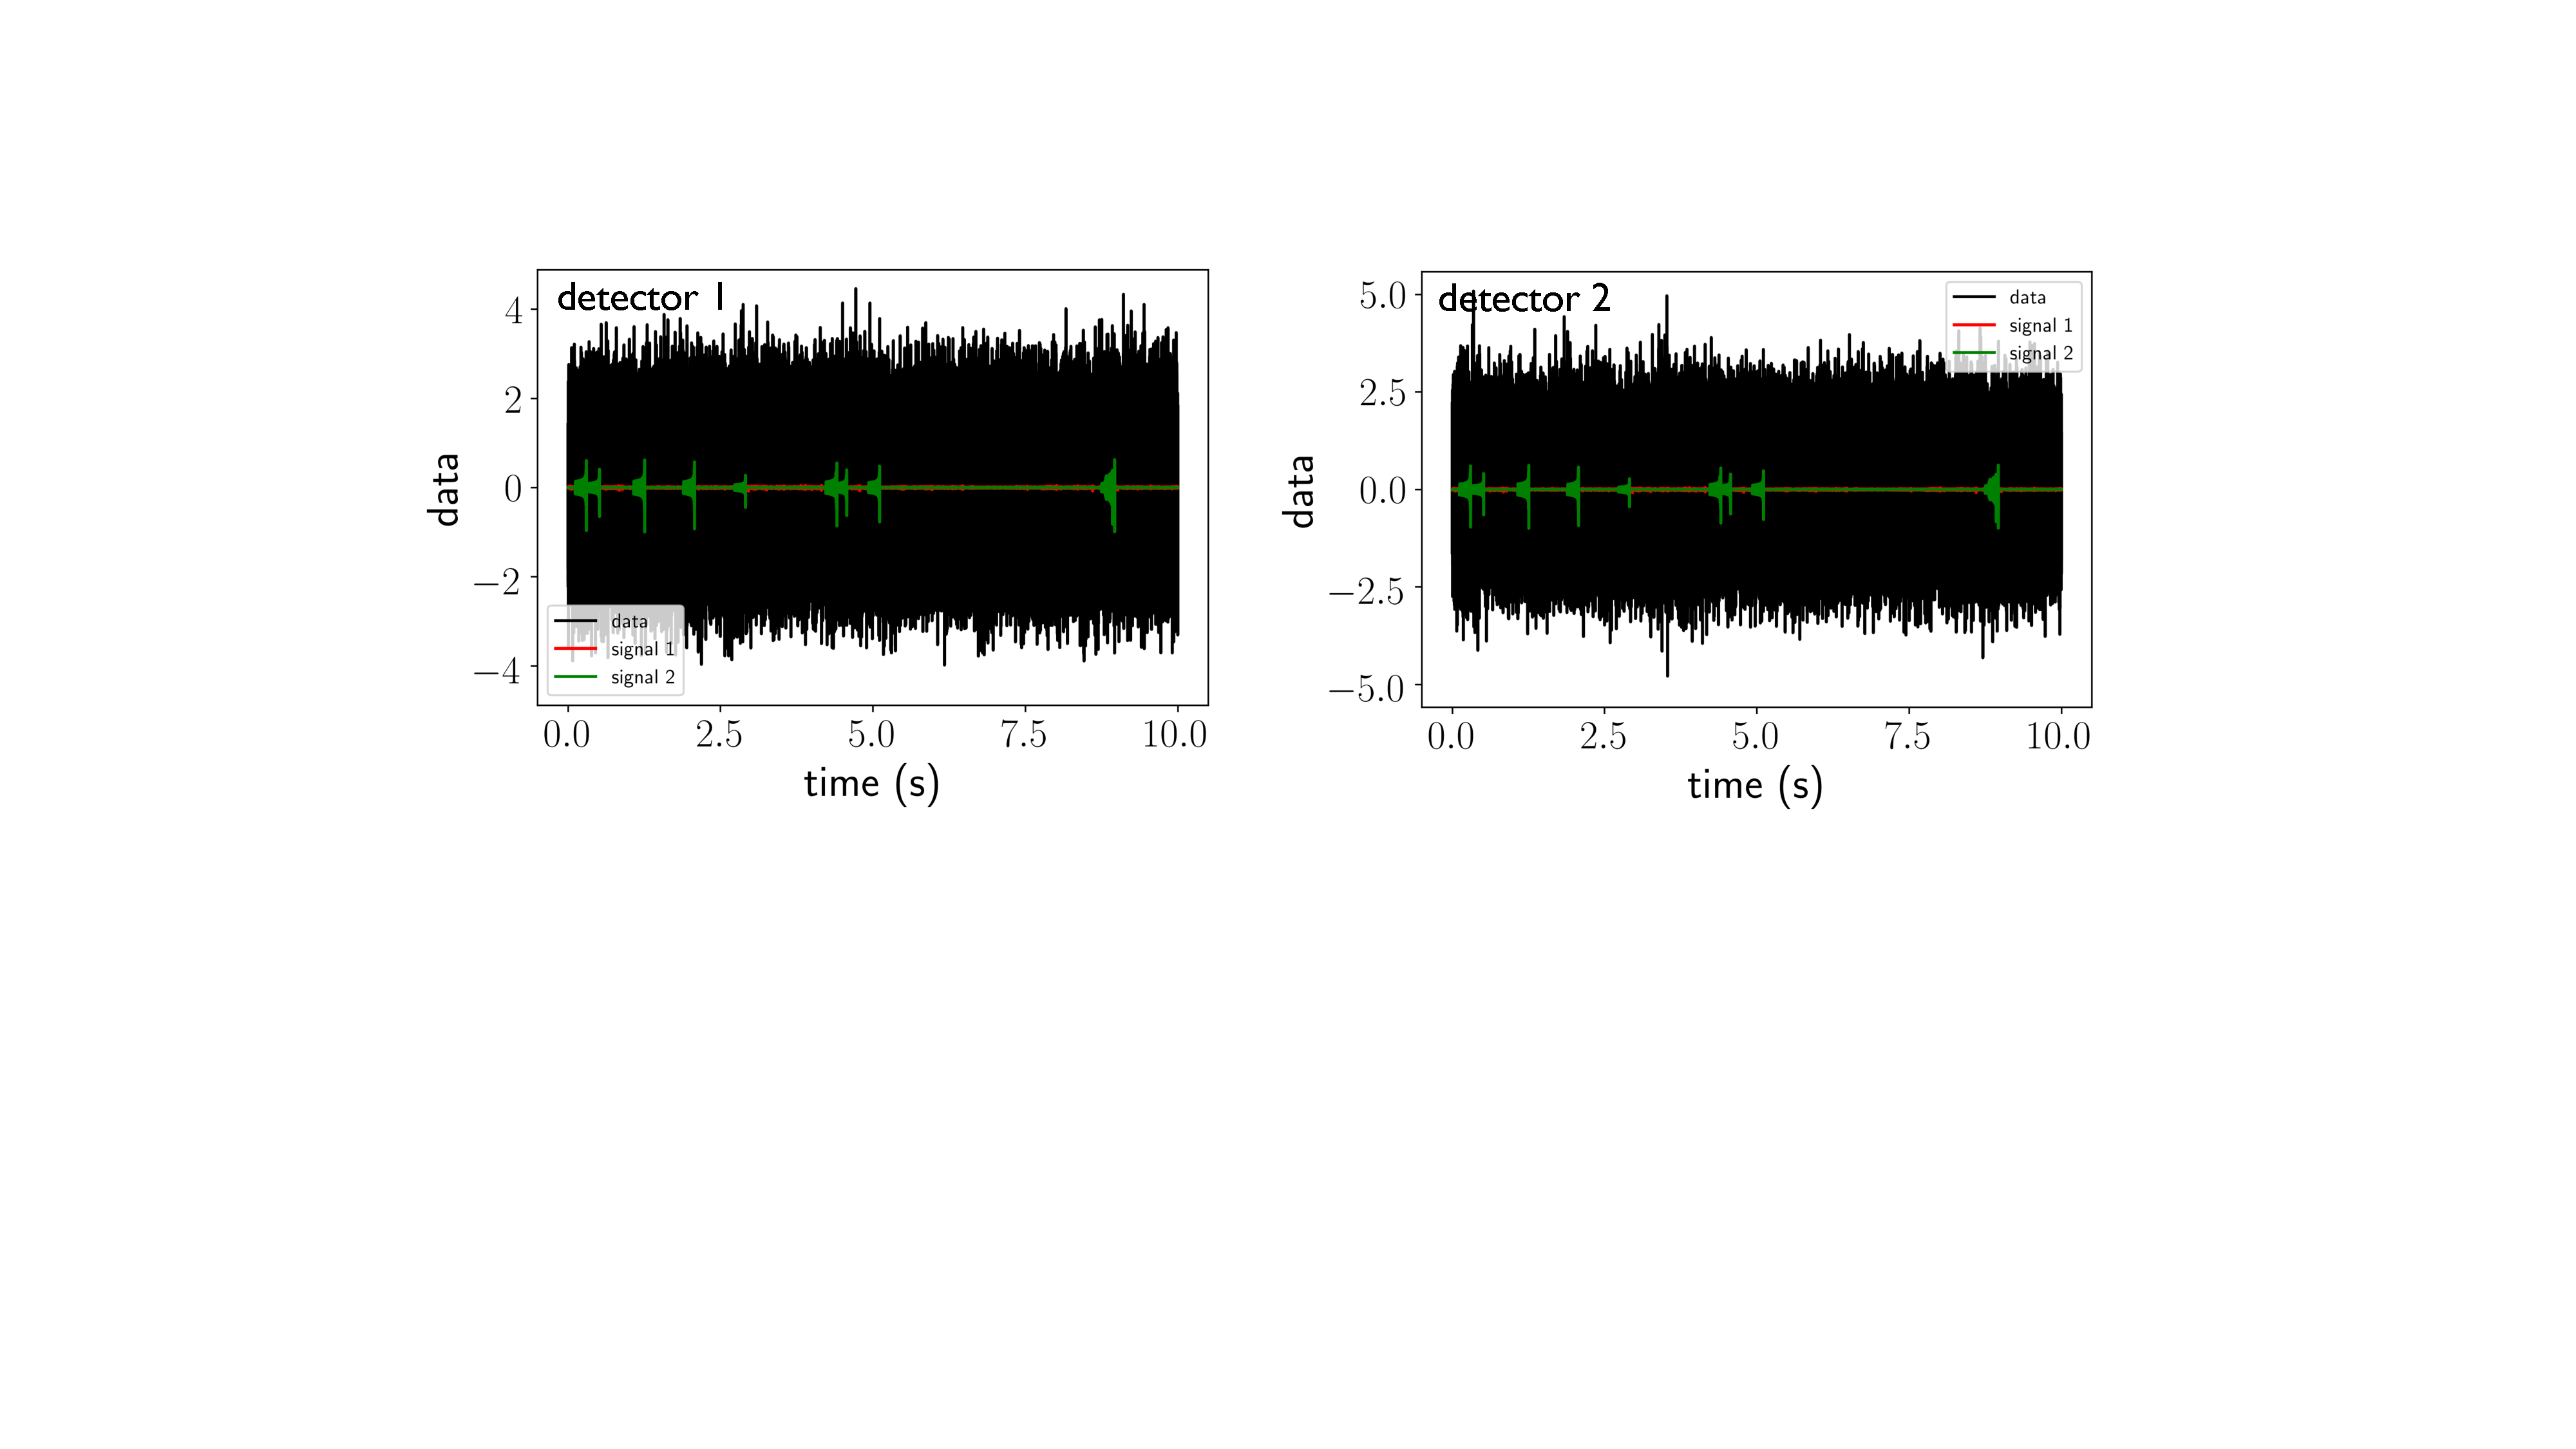
\includegraphics[width=\textwidth]{Figures/BBH-BNS-simulated-data}
\caption{Simulated BBH and BNS data in two coincident and coaligned
detectors.
The confusion-limited BNS background is shown in orange;
the popcorn-like BBH background is shown in green.
The black trace is the data consisting of the BBH and BNS signal
plus white Gaussian-stationary noise, uncorrelated in the two
detectors.}
\label{f:BBH-BNS-simulated-data}
\end{center}
\end{figure}

The final result of the analysis is the posterior distribution
for $\xi$, shown in Figure~\ref{f:posterior_xi}.
%
\begin{figure}[htbp!]
\begin{center}
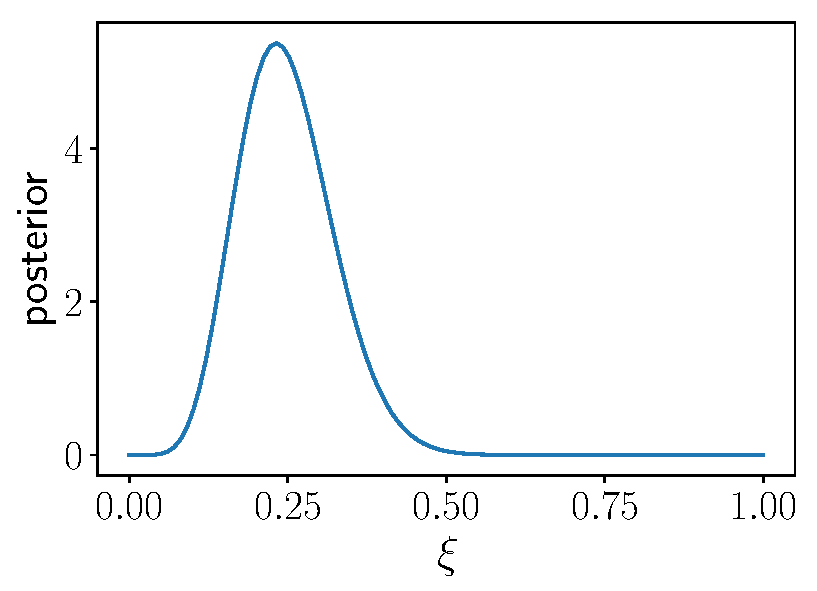
\includegraphics[width=0.4\textwidth]{Figures/posterior_xi}
\caption{The cumulative posterior distribution for $\xi$ after 
combining all 40~segments of data.}
\label{f:posterior_xi}
\end{center}
\end{figure}
%
One sees that it is peaked around the value of $\xi$ used for 
the injections, $\xi=0.25$.
Figure~\ref{f:posteriors_xi_seg} shows the posterior distributions
for $\xi$ for the first 16 segments (i.e., first 4~s) of data.
Note that these distribution are all linear in $\xi$, as to be
expected from \eqref{e:p(d_i|xi)} for the individual-segment 
likelihood functions.
In addition,
the cumulative posterior distributions for $\xi$, obtained by 
combining the likelihood functions for the first $n$ segments of
data are shown in Figure~\ref{f:posteriors_xi_cum} for 
$n=1,2,3,4,10,20,30,40$ segments.
%
\begin{figure}[htbp!]
\begin{center}
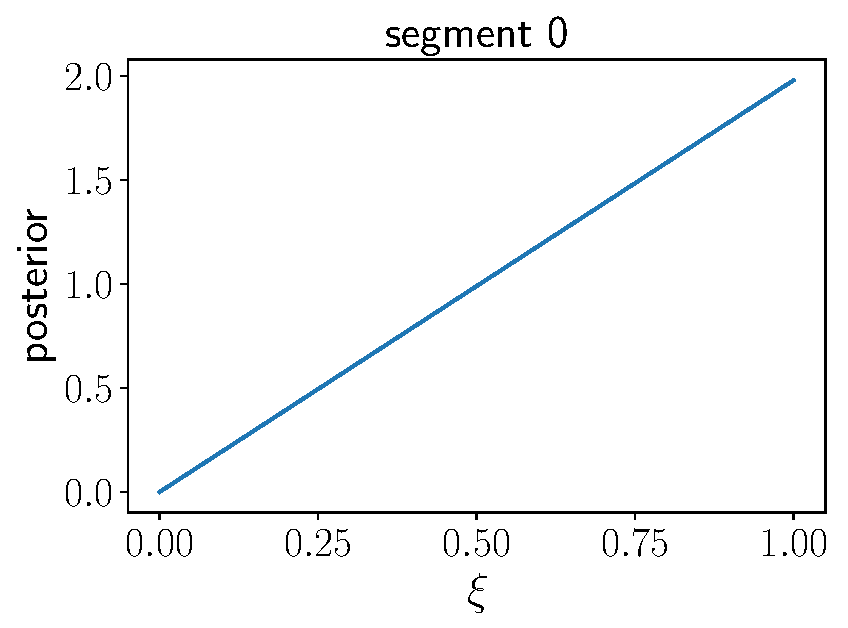
\includegraphics[width=0.24\textwidth]{Figures/posterior_xi_seg_0}
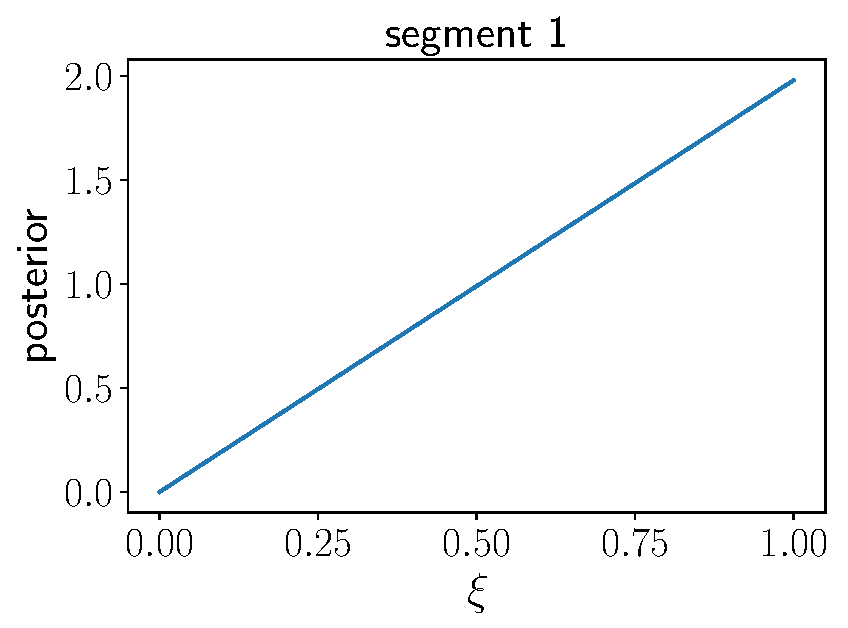
\includegraphics[width=0.24\textwidth]{Figures/posterior_xi_seg_1}
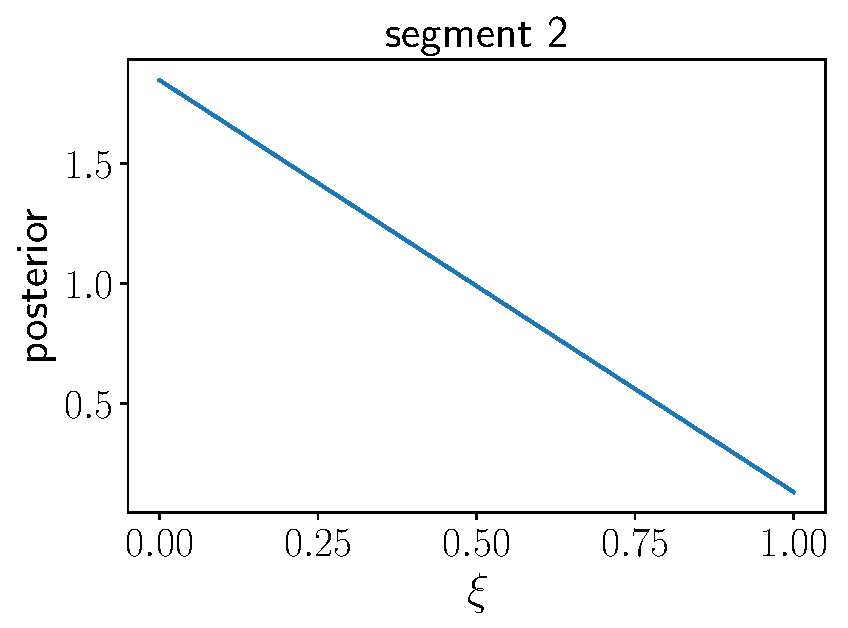
\includegraphics[width=0.24\textwidth]{Figures/posterior_xi_seg_2}
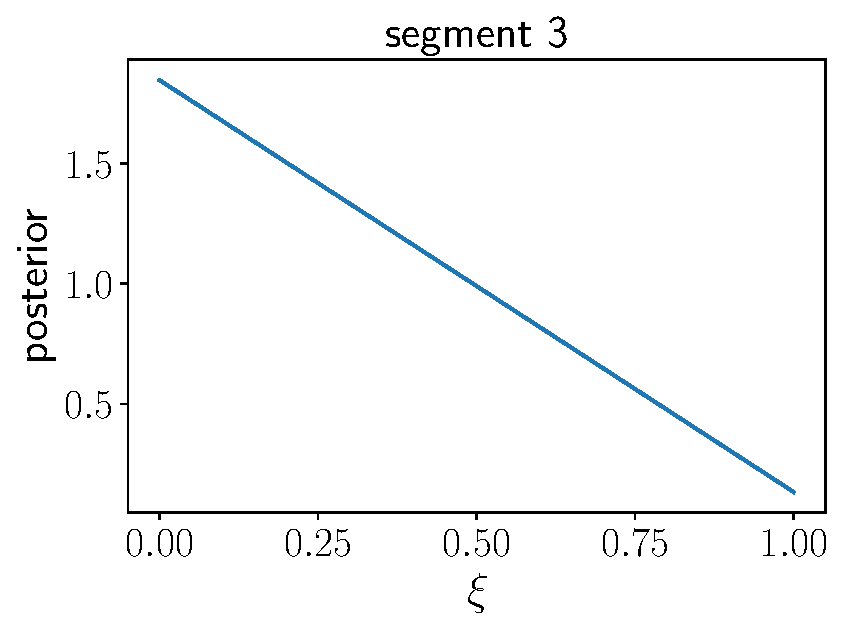
\includegraphics[width=0.24\textwidth]{Figures/posterior_xi_seg_3}
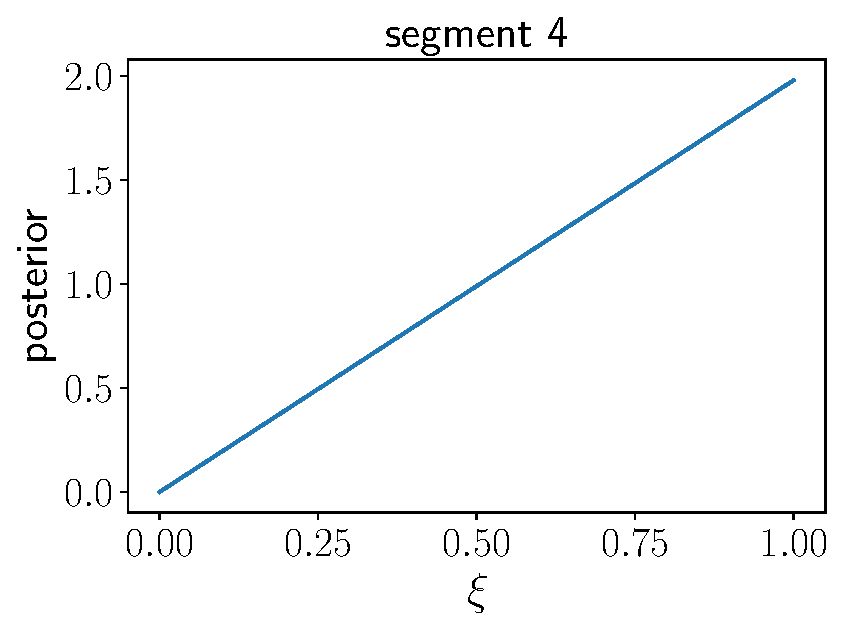
\includegraphics[width=0.24\textwidth]{Figures/posterior_xi_seg_4}
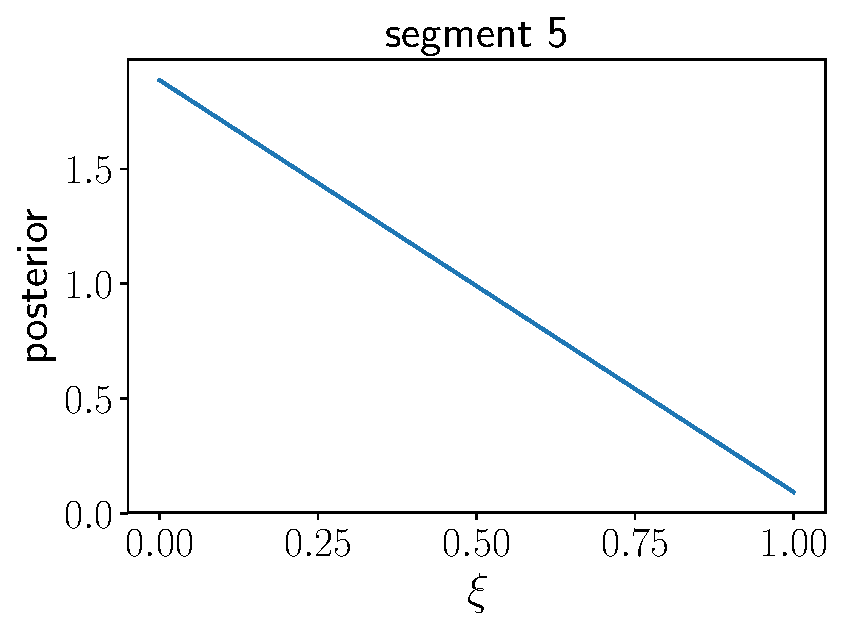
\includegraphics[width=0.24\textwidth]{Figures/posterior_xi_seg_5}
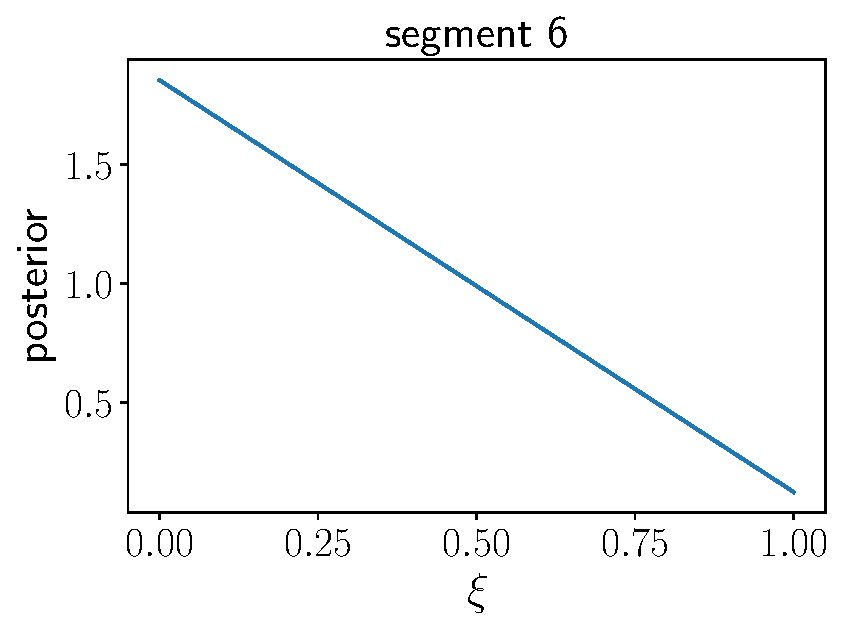
\includegraphics[width=0.24\textwidth]{Figures/posterior_xi_seg_6}
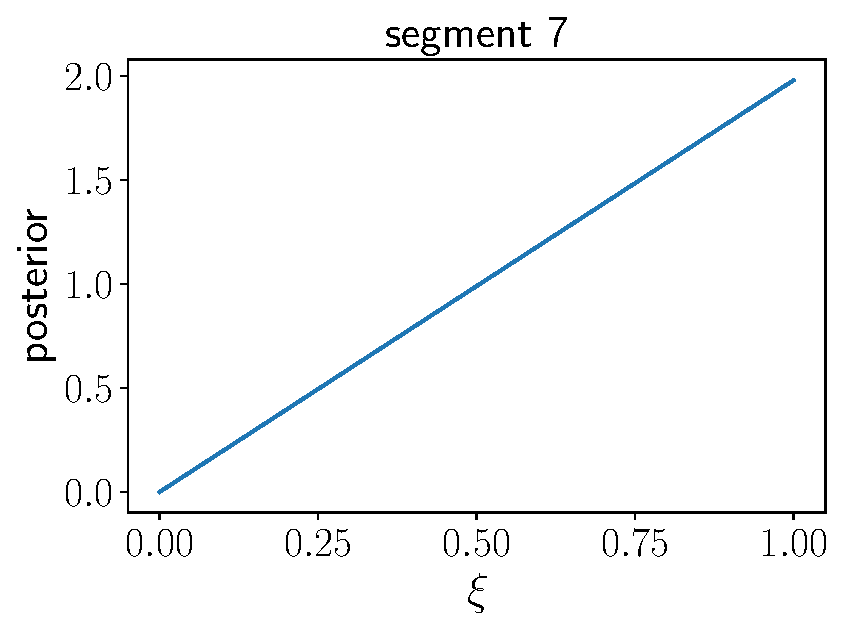
\includegraphics[width=0.24\textwidth]{Figures/posterior_xi_seg_7}
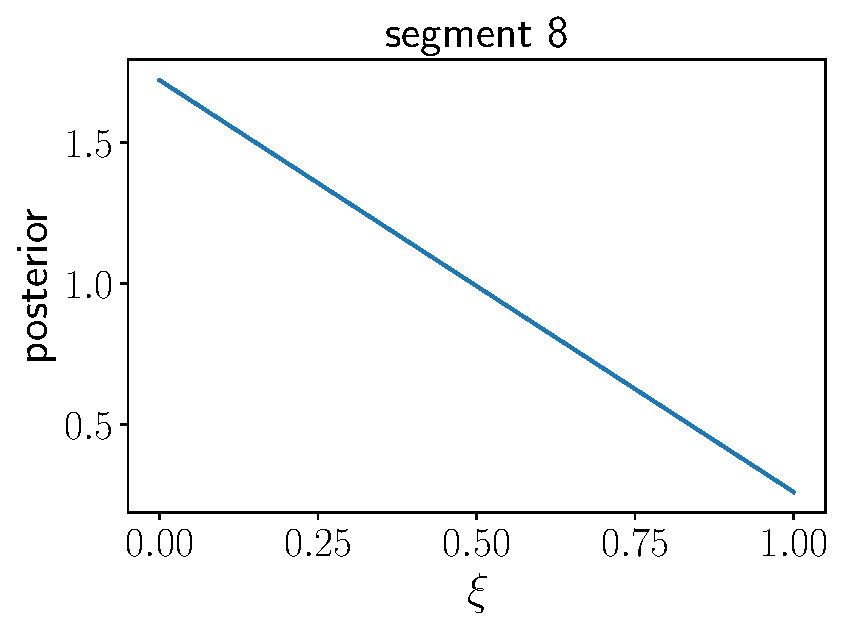
\includegraphics[width=0.24\textwidth]{Figures/posterior_xi_seg_8}
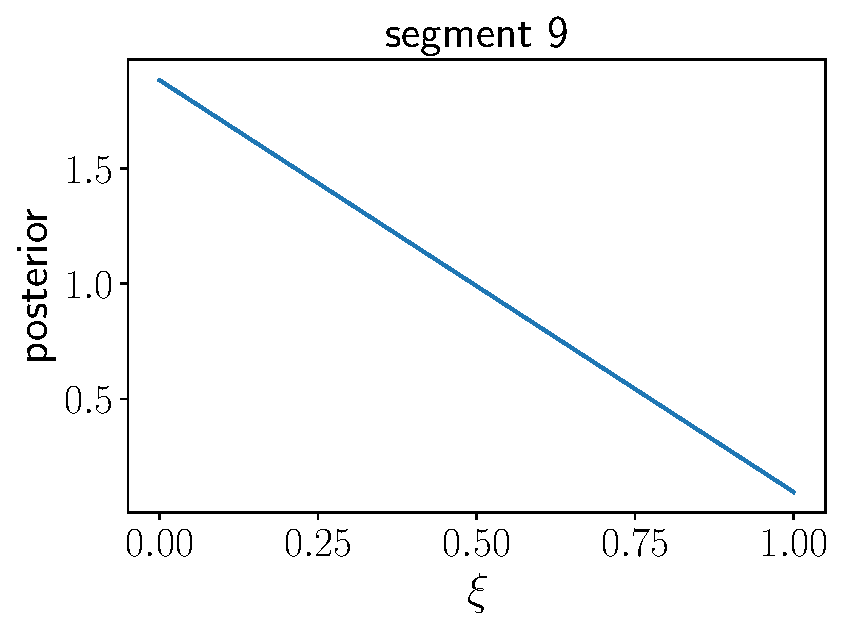
\includegraphics[width=0.24\textwidth]{Figures/posterior_xi_seg_9}
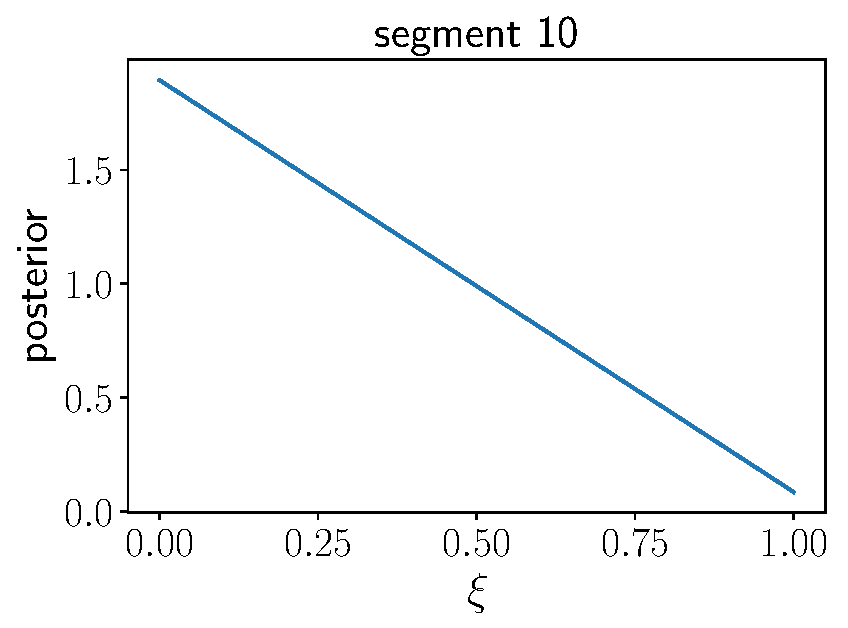
\includegraphics[width=0.24\textwidth]{Figures/posterior_xi_seg_10}
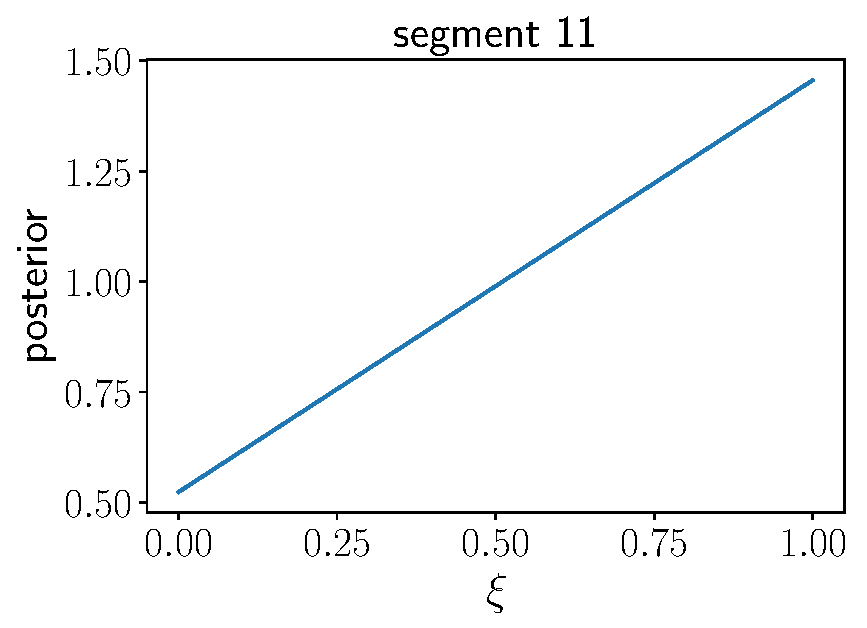
\includegraphics[width=0.24\textwidth]{Figures/posterior_xi_seg_11}
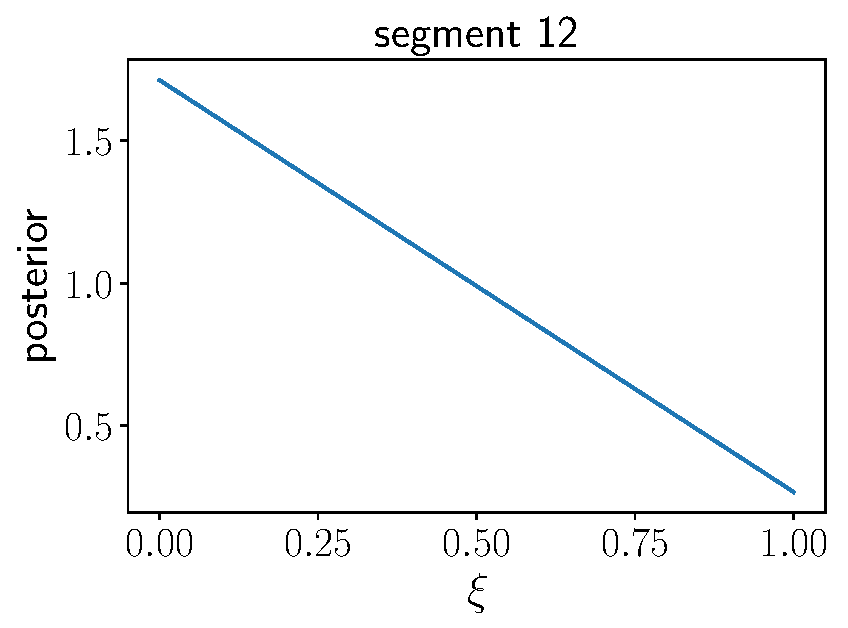
\includegraphics[width=0.24\textwidth]{Figures/posterior_xi_seg_12}
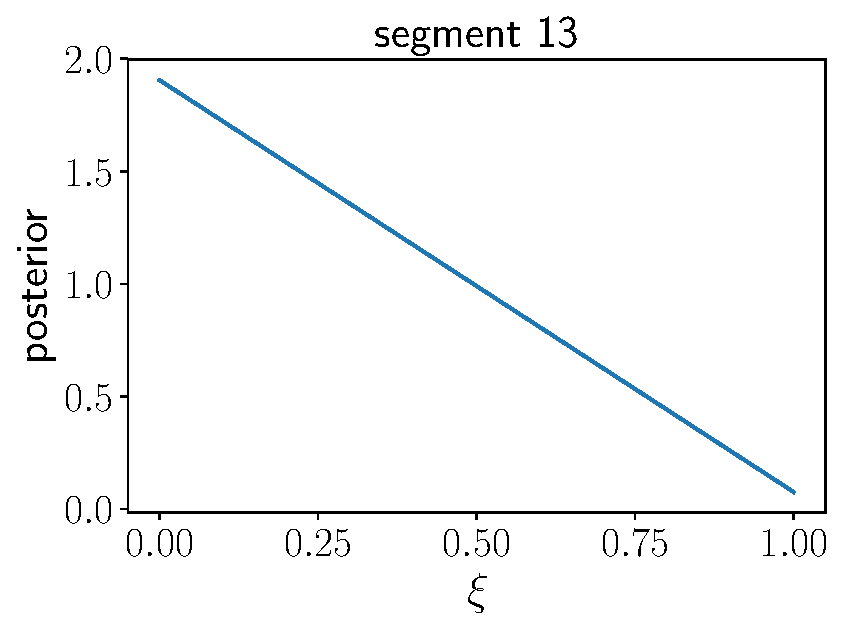
\includegraphics[width=0.24\textwidth]{Figures/posterior_xi_seg_13}
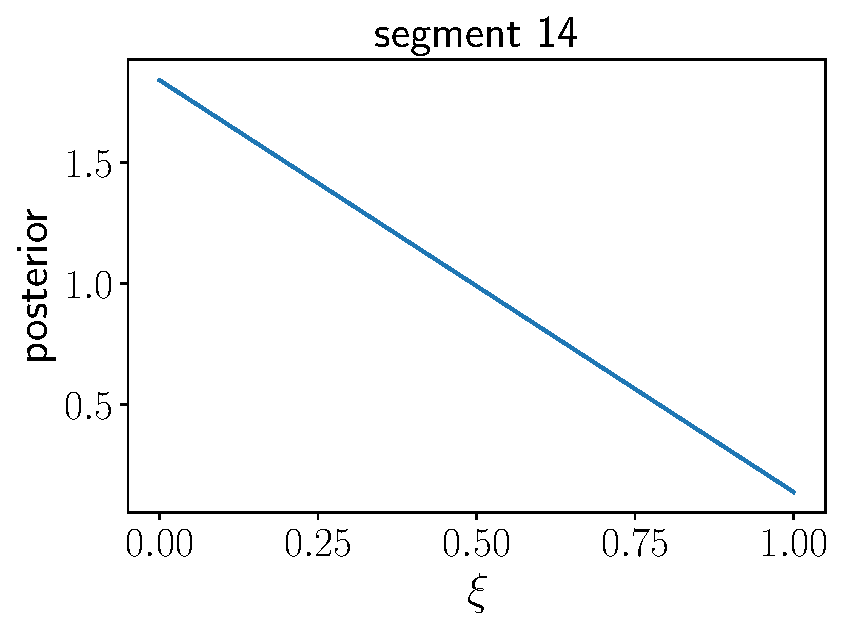
\includegraphics[width=0.24\textwidth]{Figures/posterior_xi_seg_14}
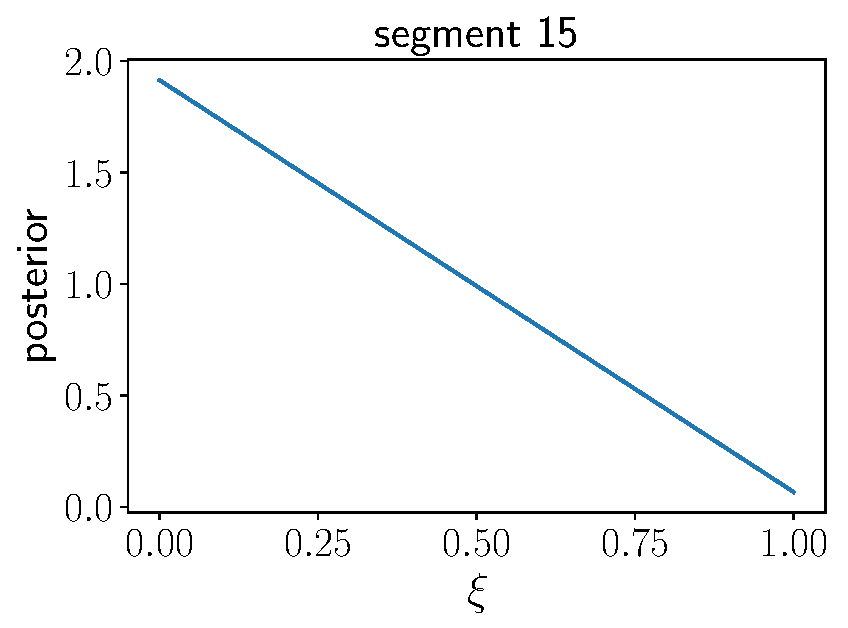
\includegraphics[width=0.24\textwidth]{Figures/posterior_xi_seg_15}
\caption{Posterior distributions for $\xi$ for the first 16 segments
(i.e., first 4~s) of data.
Since the injected signals were relatively large, the posteriors
having positive (negative) slope correspond to the segments 
having (not having) an injected BBH chirp signal.}
\label{f:posteriors_xi_seg}
\end{center}
\end{figure}
%
\begin{figure}[htbp!]
\begin{center}
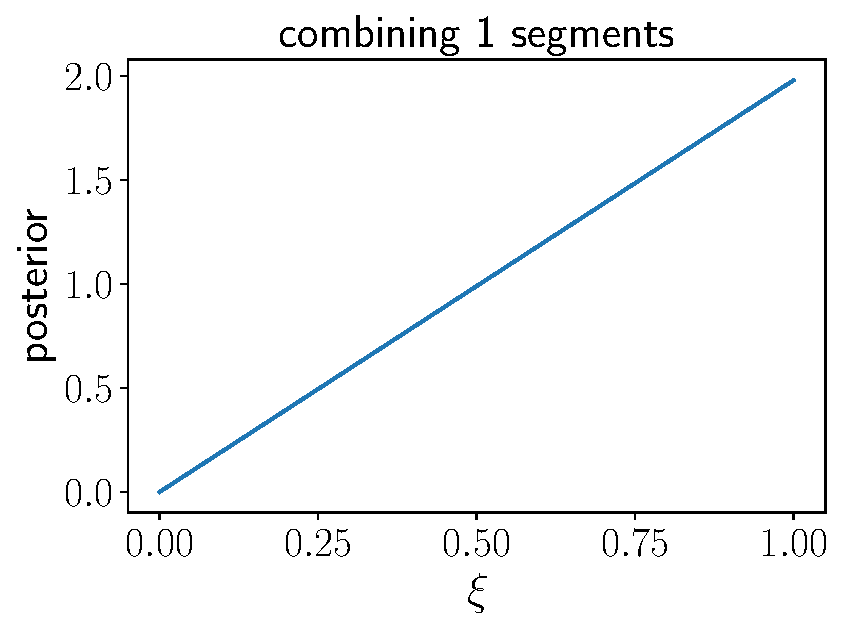
\includegraphics[width=0.24\textwidth]{Figures/posterior_xi_cum_0}
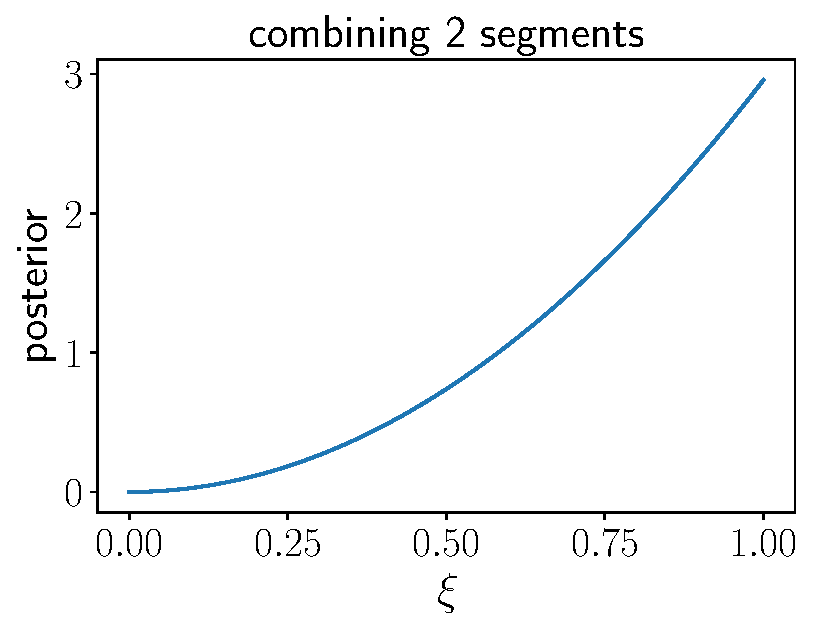
\includegraphics[width=0.24\textwidth]{Figures/posterior_xi_cum_1}
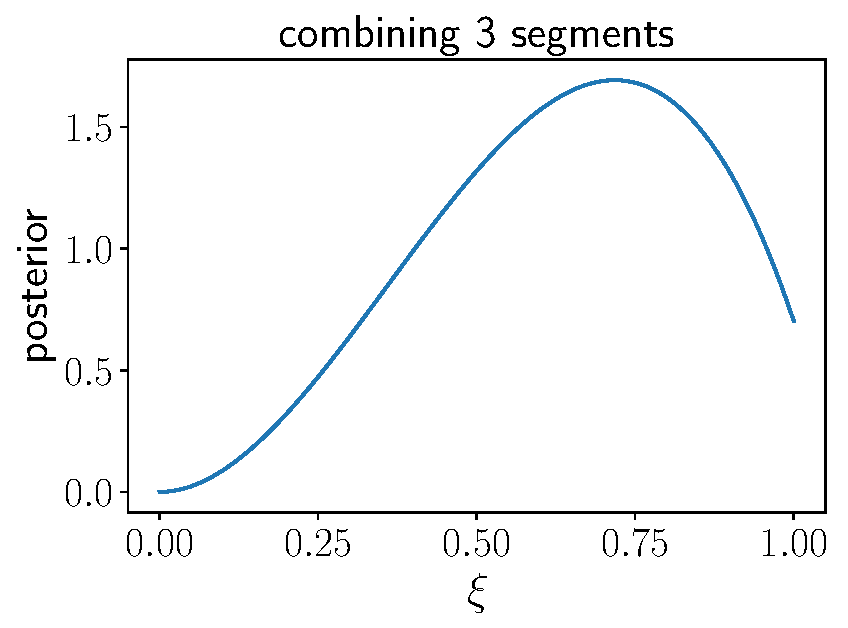
\includegraphics[width=0.24\textwidth]{Figures/posterior_xi_cum_2}
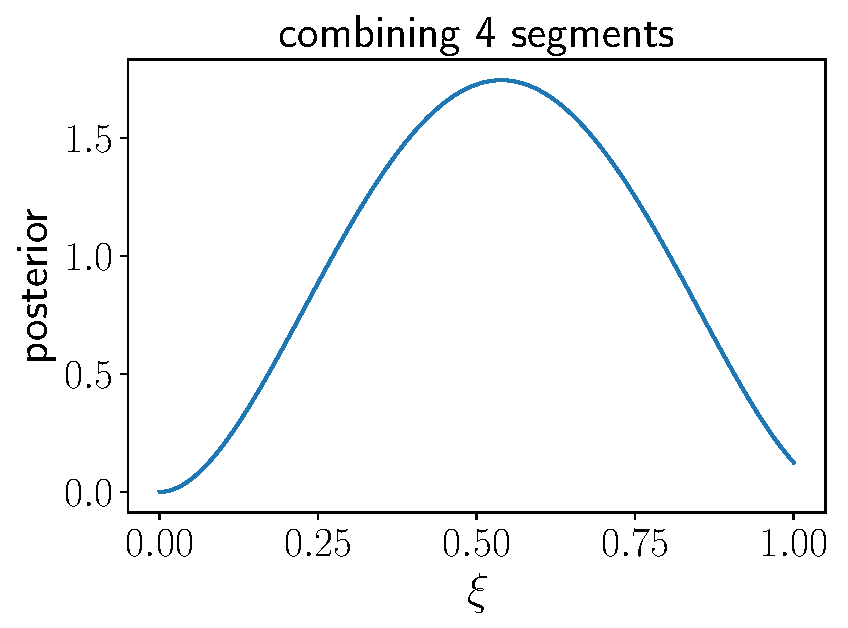
\includegraphics[width=0.24\textwidth]{Figures/posterior_xi_cum_3}
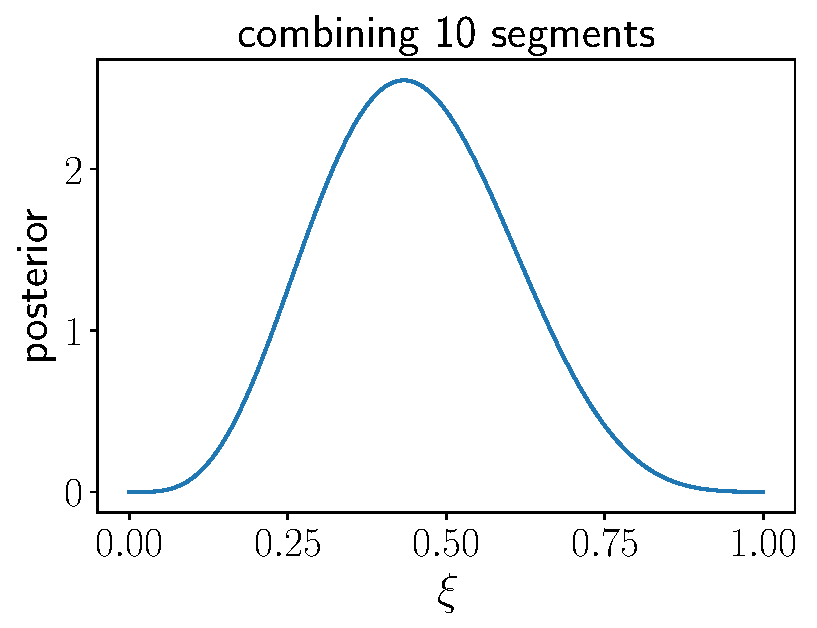
\includegraphics[width=0.24\textwidth]{Figures/posterior_xi_cum_9}
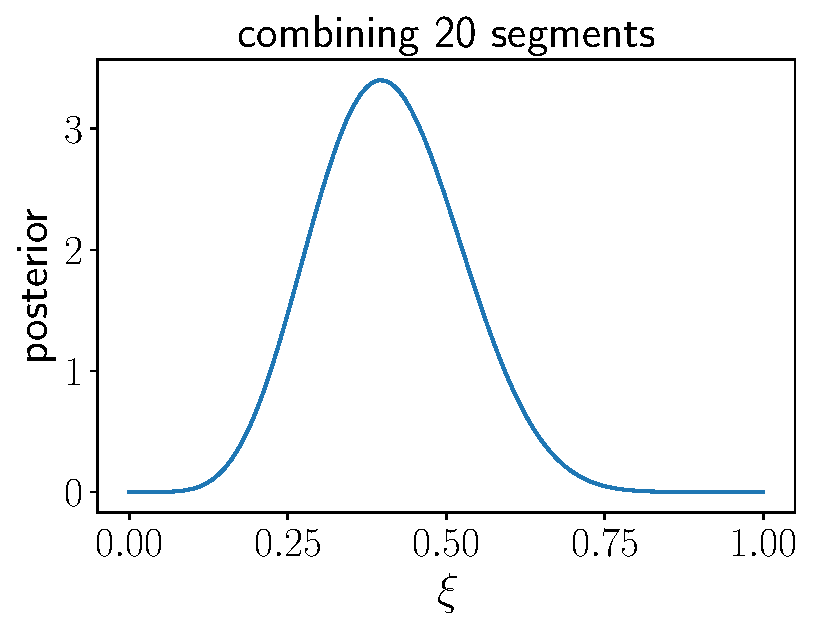
\includegraphics[width=0.24\textwidth]{Figures/posterior_xi_cum_19}
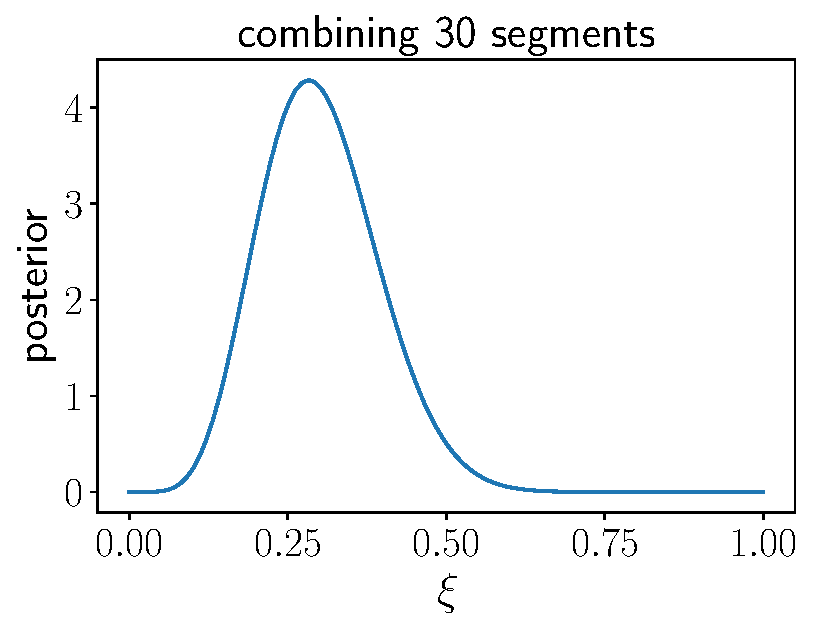
\includegraphics[width=0.24\textwidth]{Figures/posterior_xi_cum_29}
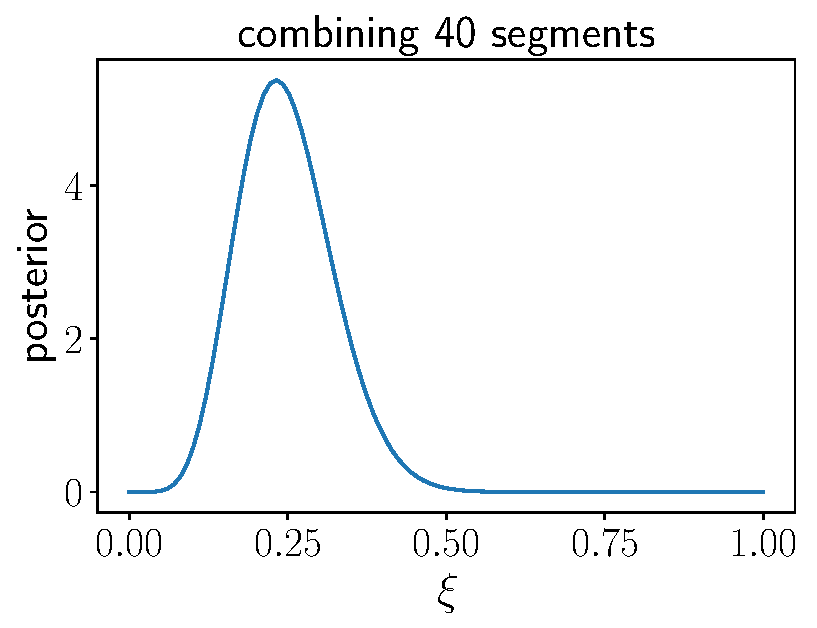
\includegraphics[width=0.24\textwidth]{Figures/posterior_xi_cum_39}
\caption{Cumulative posterior distributions for $\xi$, obtained by 
combining the likelihood functions for the first $n$ segments of data.
The bottom-rightmost plot is also shown in Figure~\ref{f:posterior_xi}.}
\label{f:posteriors_xi_cum}
\end{center}
\end{figure}
%
As $n$ increases, the product of the individual linear functions 
of $\xi$,
some with positive slope (when the evidence is in favor of the 
presence of a signal) and some with negative slope (when the 
evidence is in favor of the absence of a signal), give rise to 
a distribution that gets more and more peaked.
The bottom-rightmost part is just the final posterior distribution
shown before in Figure~\ref{f:posterior_xi}.
%

\subsection{Comparison with the standard cross-correlation search}

Of course, one can also run the standard cross-correlation search
on this data to search for the BBH background.
Although not optimal for an intermitent background like this, 
the cross-correlation method performed rather well with
%
\be
{\rm SNR}_{\rm CC} = 8.9\,.
\ee
%
This should be compared to
%
\be
{\rm SNR}_{\rm bayes} = 15.3
\ee
%
for the Bayesian search, where we used 
\eqref{e:BF-SNR} to relate a Bayesian factor to a frequentist
signal-to-noise ratio.
So the Bayesian search performed better as expected, roughly
a factor of two for this particular simulation.

The Bayesian method performs better than the standard 
cross-correlation method for the BBH background because it 
properly models the popcorn-nature of the BBH merger signals.
It uses a mixture likelihood, allowing for different 
probability distributions for those 
segments that contain a signal and those that don't.
The standard cross-correlation method, on the other hand,
treats all segments equally, looking for excess correlated
power which it can ascribe to the signal.
If most of the segments contain only noise, as is the case
for BBH merger background, the standard cross-correlation
method is going to take a longer to build up a sufficiently
signal-to-noise ratio needed to claim detection.
The standard cross-correlation method is basically measuring
the product of the duty cycle $\xi$ and the cross-correlated
power in an individual segment containing a signal.
The Bayesian method, on the other hand, is just measuring
the duty cycle $\xi$.

Note that for this Bayesian analysis, {\em all} segments contribute
to estimating the probability parameter $\xi$.

BBH chirp signal is deterministic and not stochastic.

~40 months of observation reduces to ~1 day!!
So stay tuned.

%%%%%%%%%%%%%%%%%%%%%%%%%%%%%%%%%%%%%%%%%%%%%%%%%%%
\section{Final thoughts}

The purpose of these lecture notes was to introduce the reader 
to methods used to search for stochatic GW backgrounds.
By its very nature, an introduction to a topic is necessarily
incomplete.
As such, I was only able to briefly mention stochastic 
background searches using the proposed space-based
interferometer LISA, search methods for anisotropic backgrounds, 
and for backgrounds predicted by alternative theories of gravity, etc.
The interested reader can find more detail about those topics
in~\cite{Romano-Cornish:2017} and references therein.

Although as of the time of writing these notes (summer 2019)
we have not yet detected a stochastic background, we know 
now that such a signal exists, and it's just a matter of time 
before we reach the sensitivity level needed to make a confident 
detection.
For the GWB produced by stellar-mass binary BHs throughout 
the universe, we expect to reach this level
by the time the advanced LIGO and Virgo detectors are operating
at design sensitivity (in a couple of years time).
But recall that this time-to-detection estimate is 
conservative, since it assumes that we are using the standard 
cross-correlation method, which is not optimal for 
signals that aren't on all the time.
As mentioned in Section~\ref{s:nonstationary}, there is a good 
chance that we will detect this background earlier using an 
optimal Bayesian method that properly models the popcorn-like 
nature of the BBH mergers.
But then again, pulsar timing arrays might make the first detection 
of a stochastic background, although for a different class of
source---inspiraling SMBHs in the centers of distant galaxies.
Either way, it will be an exciting time.

Finally, unlike the detection of the individually resolvable
BBH and BNS mergers, we probably
won't be able to say on one particular day that we've 
definitely detected a stochastic GW background.
Rather we will first see evidence for a background at the 
3-$\sigma$ level; and then a year or two later, we will have
evidence at the 4 or 5-$\sigma$ level.
One of the nice things about stochatic backgrounds is that
they are persistent signals (even if popcorn-like), 
so the longer we observe them, the greater our confidence in
detecting them.
And once we've confidently detected a stochastic background, 
the fun part of characterizing what we have seen begins.
As mentioned in Section~\ref{s:different_types}, different 
GW sources will produce different types of backgrounds,
so we will need to tease apart their different contributions.
And as the sensitivity of GW detectors improve, we will be 
able to observe additional structures in a background, e.g., 
anisotropies, that were not resolvable before.
Needless to say, there is plenty of work ahead of us.
